% Options for packages loaded elsewhere
\PassOptionsToPackage{unicode}{hyperref}
\PassOptionsToPackage{hyphens}{url}
%
\documentclass[
  11pt,
]{book}
\usepackage{lmodern}
\usepackage{amssymb,amsmath}
\usepackage{ifxetex,ifluatex}
\ifnum 0\ifxetex 1\fi\ifluatex 1\fi=0 % if pdftex
  \usepackage[T1]{fontenc}
  \usepackage[utf8]{inputenc}
  \usepackage{textcomp} % provide euro and other symbols
\else % if luatex or xetex
  \usepackage{unicode-math}
  \defaultfontfeatures{Scale=MatchLowercase}
  \defaultfontfeatures[\rmfamily]{Ligatures=TeX,Scale=1}
\fi
% Use upquote if available, for straight quotes in verbatim environments
\IfFileExists{upquote.sty}{\usepackage{upquote}}{}
\IfFileExists{microtype.sty}{% use microtype if available
  \usepackage[]{microtype}
  \UseMicrotypeSet[protrusion]{basicmath} % disable protrusion for tt fonts
}{}
\makeatletter
\@ifundefined{KOMAClassName}{% if non-KOMA class
  \IfFileExists{parskip.sty}{%
    \usepackage{parskip}
  }{% else
    \setlength{\parindent}{0pt}
    \setlength{\parskip}{6pt plus 2pt minus 1pt}}
}{% if KOMA class
  \KOMAoptions{parskip=half}}
\makeatother
\usepackage{xcolor}
\IfFileExists{xurl.sty}{\usepackage{xurl}}{} % add URL line breaks if available
\IfFileExists{bookmark.sty}{\usepackage{bookmark}}{\usepackage{hyperref}}
\hypersetup{
  pdftitle={FishPath Tool User Guide},
  pdfauthor={The Nature Conservancy},
  hidelinks,
  pdfcreator={LaTeX via pandoc}}
\urlstyle{same} % disable monospaced font for URLs
\usepackage{longtable,booktabs}
% Correct order of tables after \paragraph or \subparagraph
\usepackage{etoolbox}
\makeatletter
\patchcmd\longtable{\par}{\if@noskipsec\mbox{}\fi\par}{}{}
\makeatother
% Allow footnotes in longtable head/foot
\IfFileExists{footnotehyper.sty}{\usepackage{footnotehyper}}{\usepackage{footnote}}
\makesavenoteenv{longtable}
\usepackage{graphicx,grffile}
\makeatletter
\def\maxwidth{\ifdim\Gin@nat@width>\linewidth\linewidth\else\Gin@nat@width\fi}
\def\maxheight{\ifdim\Gin@nat@height>\textheight\textheight\else\Gin@nat@height\fi}
\makeatother
% Scale images if necessary, so that they will not overflow the page
% margins by default, and it is still possible to overwrite the defaults
% using explicit options in \includegraphics[width, height, ...]{}
\setkeys{Gin}{width=\maxwidth,height=\maxheight,keepaspectratio}
% Set default figure placement to htbp
\makeatletter
\def\fps@figure{htbp}
\makeatother
\setlength{\emergencystretch}{3em} % prevent overfull lines
\providecommand{\tightlist}{%
  \setlength{\itemsep}{0pt}\setlength{\parskip}{0pt}}
\setcounter{secnumdepth}{5}
\usepackage{booktabs}
\usepackage[]{natbib}
\bibliographystyle{apalike}

\title{FishPath Tool User Guide}
\author{The Nature Conservancy}
\date{Last updated: March 25, 2021}

\begin{document}
\maketitle

{
\setcounter{tocdepth}{1}
\tableofcontents
}
\hypertarget{section}{%
\chapter*{}\label{section}}
\addcontentsline{toc}{chapter}{}

\begin{center}
\includegraphics[width=0.75\linewidth]{images/3-logos} \end{center}

\hypertarget{intro}{%
\chapter{Introduction}\label{intro}}

\hypertarget{motivation}{%
\section{Motivation for Developing the FishPath Tool and FishPath Process}\label{motivation}}

Well-managed, sustainable fisheries have a few common elements no matter the circumstance - the rules that govern sustainable fisheries practices are transparent, supported by stakeholders, and tailored to the fishery context. More technically, this involves collecting data, which feed into an assessment, and then using assessment results to inform management measures. However, only a small fraction of the world's fisheries have these sustainable management systems in place, with resource- and data-limited fisheries facing significant challenges in their development. Notable recent progress has been achieved in the development of stock assessments and other data-limited tools, but outstanding challenges for data-limited fisheries lie in selecting and implementing appropriate options for data collection, stock assessment, and management measures --- the key components of a harvest strategy.

Due to a wide variety of possibilities, understanding the full suite of available data collection, stock assessment, and management measure options and choosing the options most appropriate for each fishery is often a daunting process. Exacerbating the challenge of numerous options, data-limited fisheries are often simultaneously capacity- or resource-limited. In addition, small-scale fisheries have unique characteristics and challenges which require tailored plans. Singular or generic approaches that do not fully consider the entire fishery's unique challenges must be avoided. An enormous challenge lies in broadening the accessibility of technical information, resources, and harvest strategy support tools, while not oversimplifying the innate complexity and nuanced aspects of each individual fishery setting.

FishPath was created to address these challenges. It was developed through a collaboration between The Nature Conservancy (TNC), the U.S. National Oceanic and Atmospheric Administration (NOAA), and Australia's Commonwealth Scientific and Industrial Research Organisation (CSIRO). FishPath is an approach for setting fisheries on the path to sustainability. The FishPath approach streamlines something that everyone working in fisheries strives to do --- figure out what to do with what you have. It provides an organized, efficient and inclusive way to do it.

The overall FishPath approach includes a stakeholder engagement process which is underpinned by the FishPath Tool. The broader FishPath Process aims to engage stakeholders and build capacity to develop management measures that are tailored to local conditions and challenges. The FishPath Tool supports the process of identifying viable components of the management strategy.

\hypertarget{fishpath-tool-overview}{%
\section{FishPath Tool Overview}\label{fishpath-tool-overview}}

The FishPath Tool is an online decision-support tool for data-limited fisheries management. The primary goal of the FishPath Tool is to support users in understanding and refining options for the three major components of a harvest strategy: 1) data collection, 2) data-limited assessment, and 3) management measures.

The FishPath Tool uses multiple-choice questions to determine unique characteristics of the fishery (Figure \ref{fig:overview}). Questions cover social, economic, operational, biological, ecological and governance characteristics, and which types of data are available. The FishPath Tool contains a database of about 50 options for each of the 3 sections (data collection, assessment, management measures). The answers to the questionnaire flag key assumptions, considerations, and cautions for each option contained in the FishPath Tool. This guidance is based on the fishery context and can be used to understand the appropriateness of each option for the fishery of interest. The Tool results section provides a guided process for narrowing down available options to a short list to be more formally considered for inclusion in a harvest strategy (Figure \ref{fig:overview}). Users can also learn about each option through details, resources and links within the Tool.

It is important to understand what the FishPath Tool does and does not do. First, the FishPath Tool is not quantitative -- it does not input, upload, or analyze data. The FishPath Tool is not a simulation or stock assessment Tool. The FishPath Tool does aid in the process of identifying a short list of viable options, but it does not prescribe a single, preferred option for data collection, assessment, or management measures. Rather, it encourages critical evaluation of an identified subset of options. The FishPath Tool provides a transparent and efficient platform for users to build the foundation of a harvest strategy for data-limited fisheries. The FishPath Tool content undergoes continual updates to include the latest fisheries science and practitioner information. FishPath Tool users may submit content suggestions at \href{mailto:support@fishpath.org}{\nolinkurl{support@fishpath.org}}.

\begin{figure}

{\centering 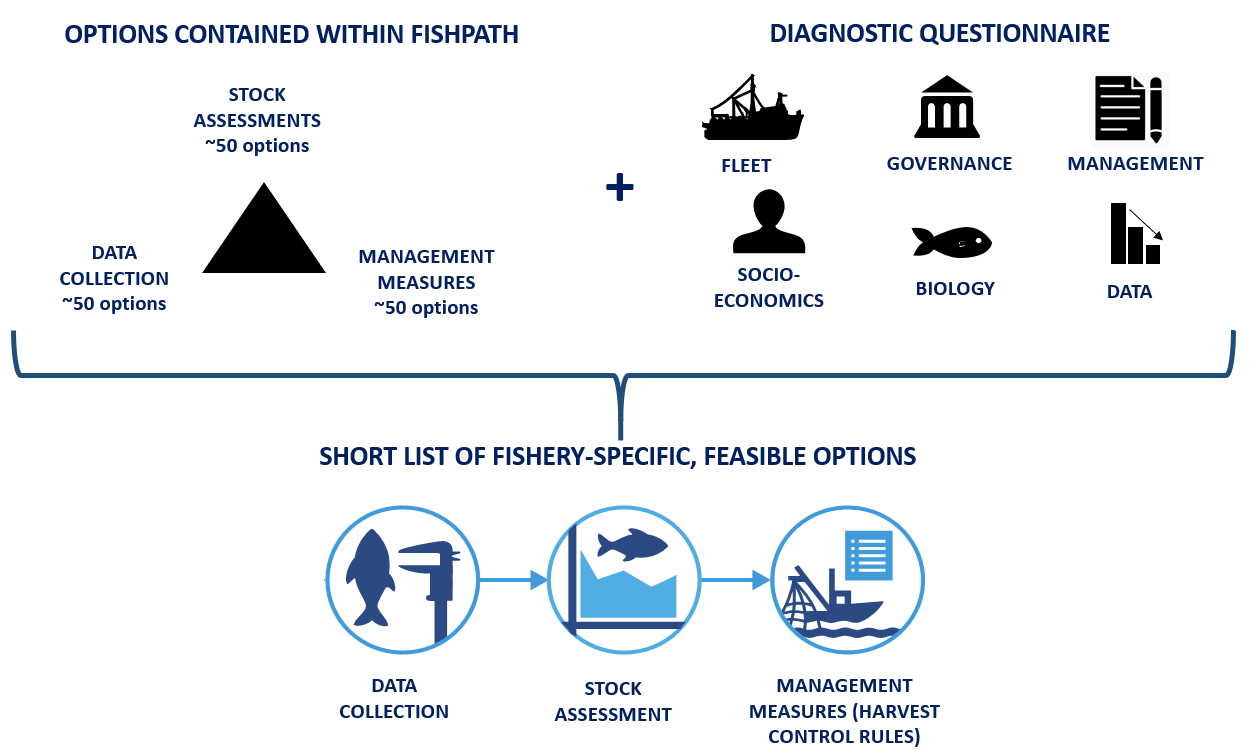
\includegraphics[width=0.75\linewidth]{images/fishpath-tool-overview-diagram} 

}

\caption{The FishPath Tool at a glance.}\label{fig:overview}
\end{figure}

\hypertarget{intended-audience-and-use-of-the-fishpath-tool}{%
\section{Intended Audience and Use of the FishPath Tool}\label{intended-audience-and-use-of-the-fishpath-tool}}

The FishPath Tool is intended to be used in two key settings. The first setting is with a trained FishPath Tool facilitator, and the second as an individual user. Each of these intended audience groups may have varying levels of fisheries science and management experience.

\hypertarget{i.-tool-use-in-facilitated-engagement-process-or-workshop}{%
\subsubsection{I. Tool Use in Facilitated Engagement Process or Workshop:}\label{i.-tool-use-in-facilitated-engagement-process-or-workshop}}

The FishPath Tool is designed to be navigated by a trained fisheries scientist who facilitates the use of the tool in a group setting with fishery stakeholders. These stakeholders can be multi- (e.g., scientists, managers, universities, fishing industry) or single- (e.g., agency scientists) stakeholder groups. The trained FishPath facilitator leads discussion around answering the FishPath Tool questionnaire and process of narrowing results. In this setting, the overall FishPath Process, led by the facilitator, bridges or lessens any potential gaps related to the technical terms and concepts presented in the tool, improving accessibility to stakeholders. In this setting, the audience members in the meeting are experts in the focal fishery (including fishermen) or familiar with fisheries science and management, but do not need to be career, quantitative fisheries science experts.

\hypertarget{ii.-tool-use-as-individual-user}{%
\subsubsection{II. Tool Use as Individual User:}\label{ii.-tool-use-as-individual-user}}

The FishPath Tool is also intended to be used by individuals or groups without the support of a trained FishPath facilitator (also referred to as ``Desktop Users'' or those who use the FishPath Tool on their own). These individuals have an intermediate to advanced working knowledge of fisheries science and management. To fully understand the tool and apply it correctly, it is recommended that these users read and thoroughly digest this FishPath Tool User Guide. Examples of individual users include:

\begin{itemize}
\tightlist
\item
  Fisheries scientists, researchers, or students, who are interested in identifying appropriate data-limited assessment options for a data-limited fishery;
\item
  Fisheries scientists, managers, students, or other fisheries professionals who want to review and corroborate existing harvest strategy components against guidance provided by FishPath;
\item
  Fisheries scientists, managers, students, or other fisheries professionals seeking reference material or a fisheries resource library related to data-limited fisheries management.
\end{itemize}

The purpose of this User Guide is to explain Tool functionality and provide guidance on how to use the FishPath Tool to select and review appropriate options for data collection, data-limited assessment, and management measures.

\hypertarget{starting-the-fishpath-tool}{%
\chapter{Starting the FishPath Tool}\label{starting-the-fishpath-tool}}

Importantly, the FishPath Tool requires a consistent internet connection to access the questionnaire, save answers, and interact with results.

\hypertarget{welcome-page}{%
\section{Welcome Page}\label{welcome-page}}

When a user navigates to \url{https://tool.fishpath.org/}, a welcome page is displayed with two prompts: ``Create an Account'' or ``Login'' (Figure \ref{fig:welcome}).

\begin{figure}

{\centering 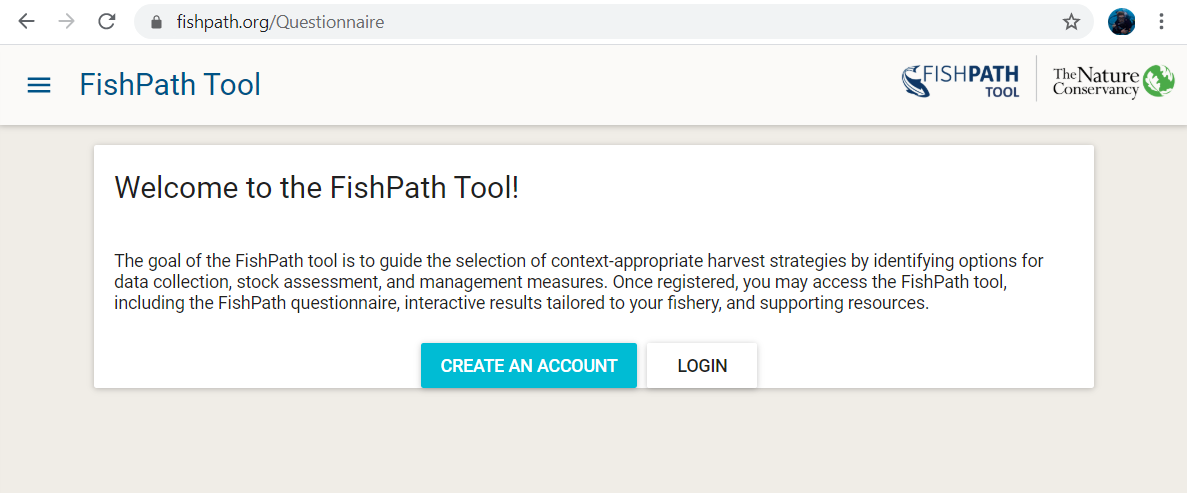
\includegraphics[width=0.95\linewidth]{images/welcome-page} 

}

\caption{Welcome page of the FishPath Tool.}\label{fig:welcome}
\end{figure}

\hypertarget{creating-a-fishpath-account}{%
\section{Creating a FishPath Account}\label{creating-a-fishpath-account}}

Upon selecting ``Create an Account'', a pop-up window appears with the following fill-in fields (Figure \ref{fig:create-account}). An asterisk denotes mandatory information.

\begin{itemize}
\tightlist
\item
  Email*
\item
  Password* (create a password)
\item
  Organization Type*
\item
  Organization
\item
  Your Name*
\item
  Country*
\end{itemize}

Note that the email and password fields are case sensitive.

This information is used to track user origin and the use of the FishPath tool. At this account creation stage, the user is also prompted to read and accept the Terms of Service of the FishPath tool, developed by The Nature Conservancy (\protect\hyperlink{terms}{Appendix B}).

\begin{figure}

{\centering 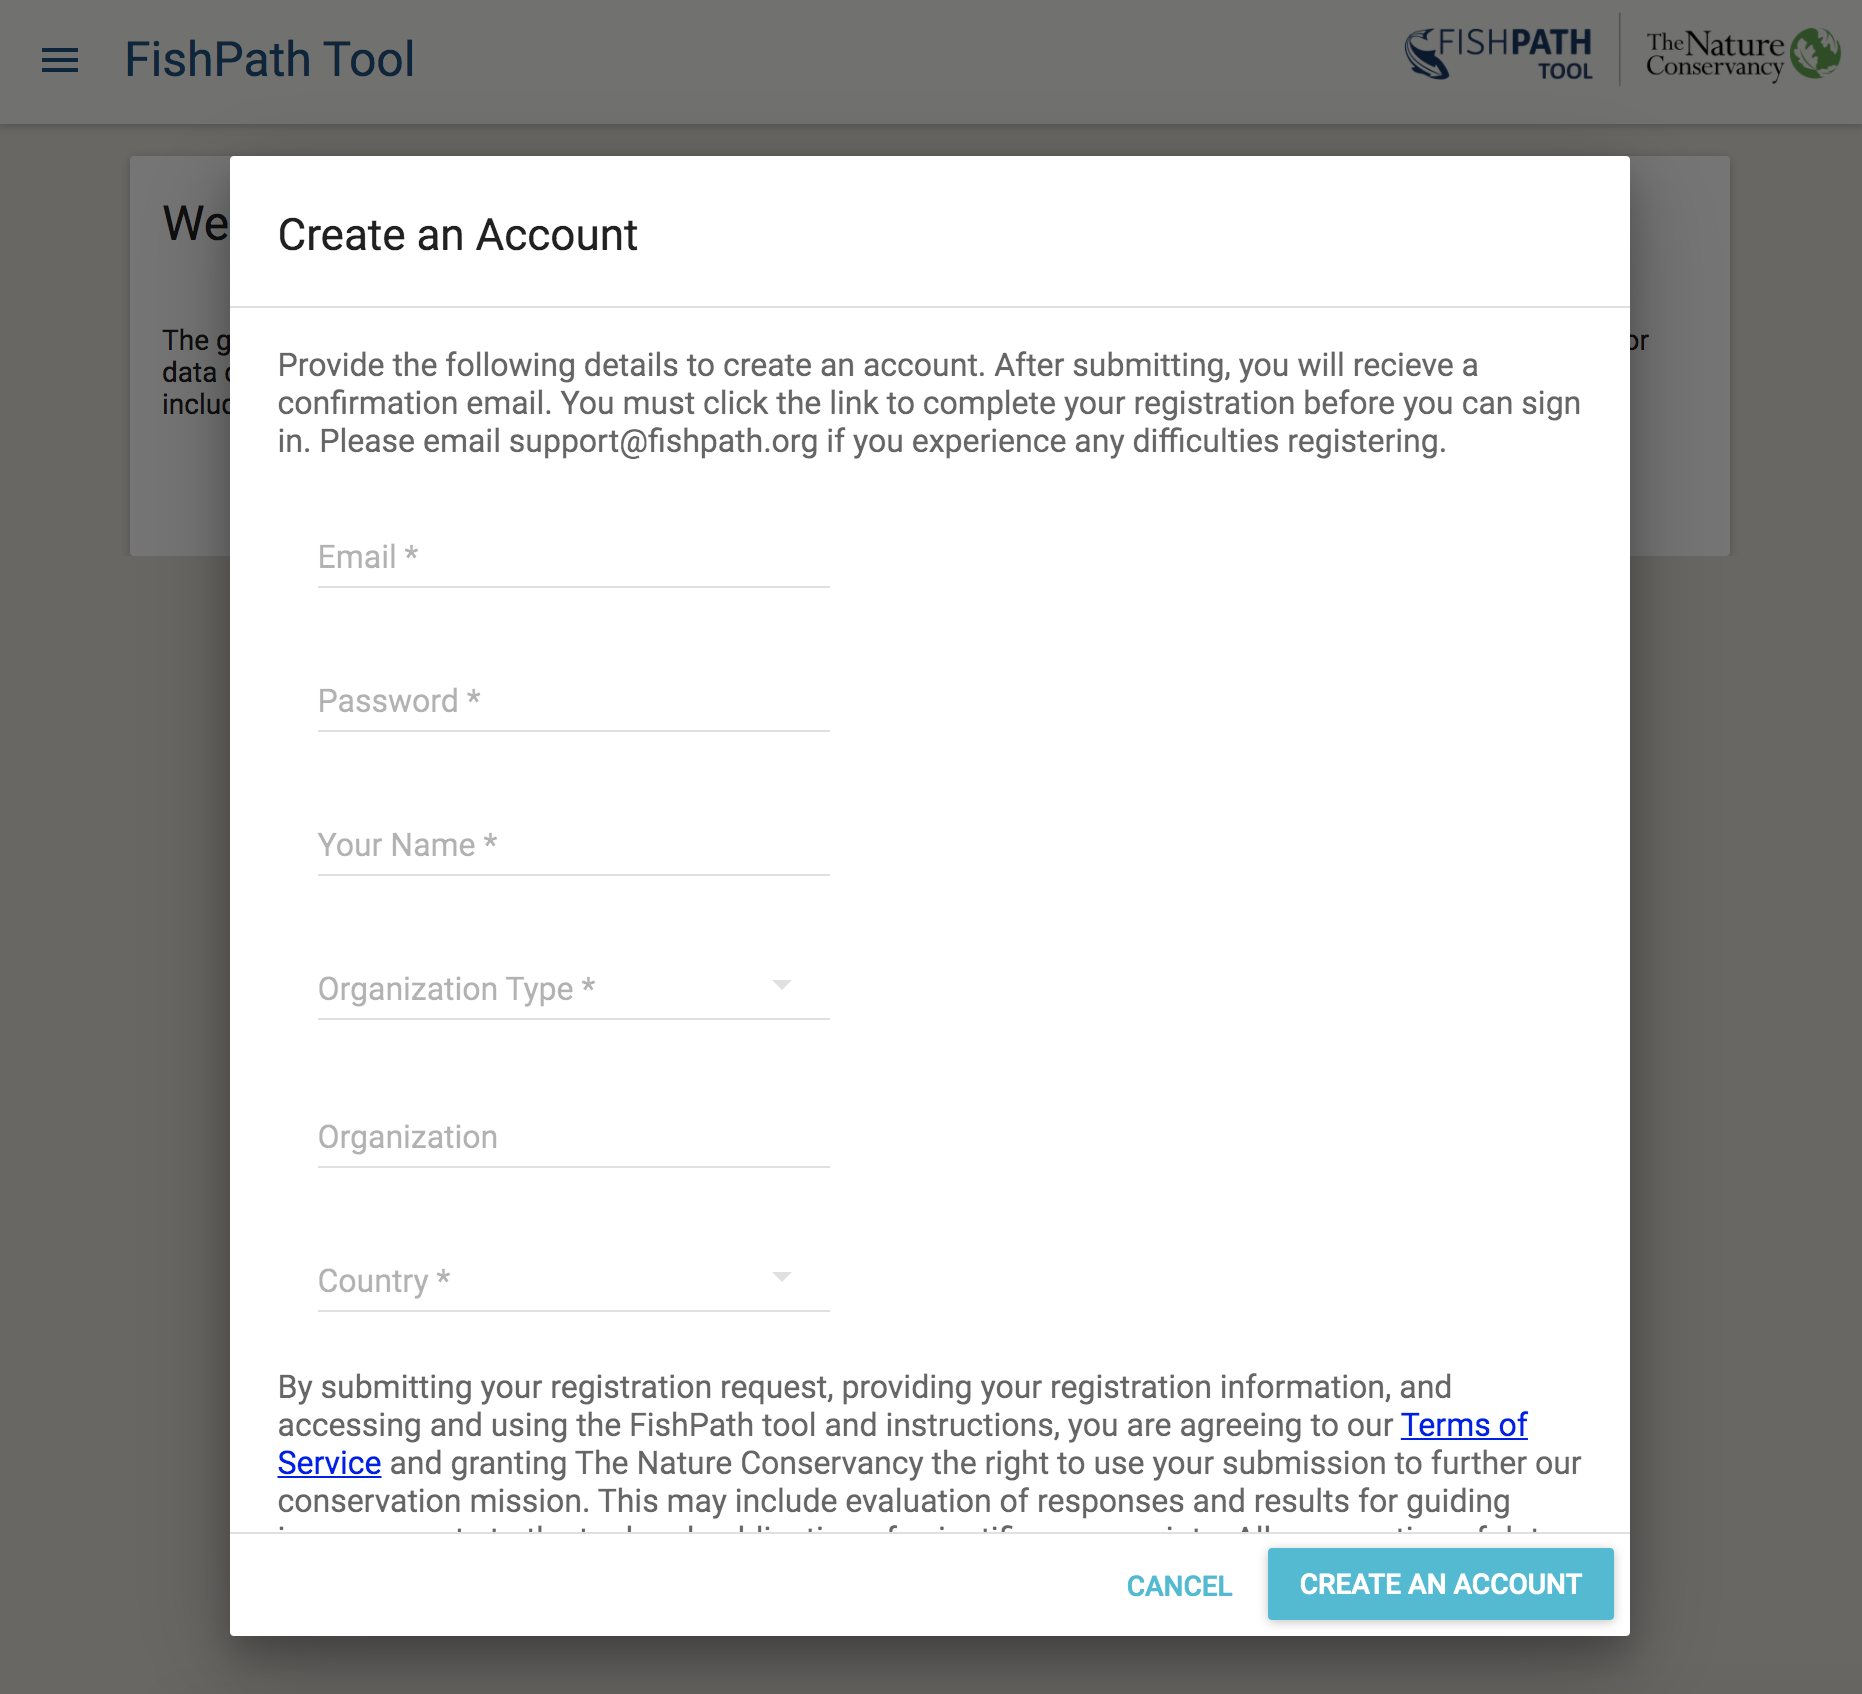
\includegraphics[width=0.95\linewidth]{images/create-account} 

}

\caption{“Create an Account” screen of the FishPath Tool.}\label{fig:create-account}
\end{figure}

After submitting the account request, the user will automatically receive a confirmation email with a link to complete registration. After account creation, whenever the user returns to the Welcome Page of the FishPath Tool, the user may simply ``Login'' with their email address and password (Figure \ref{fig:login-page}).

\begin{figure}

{\centering 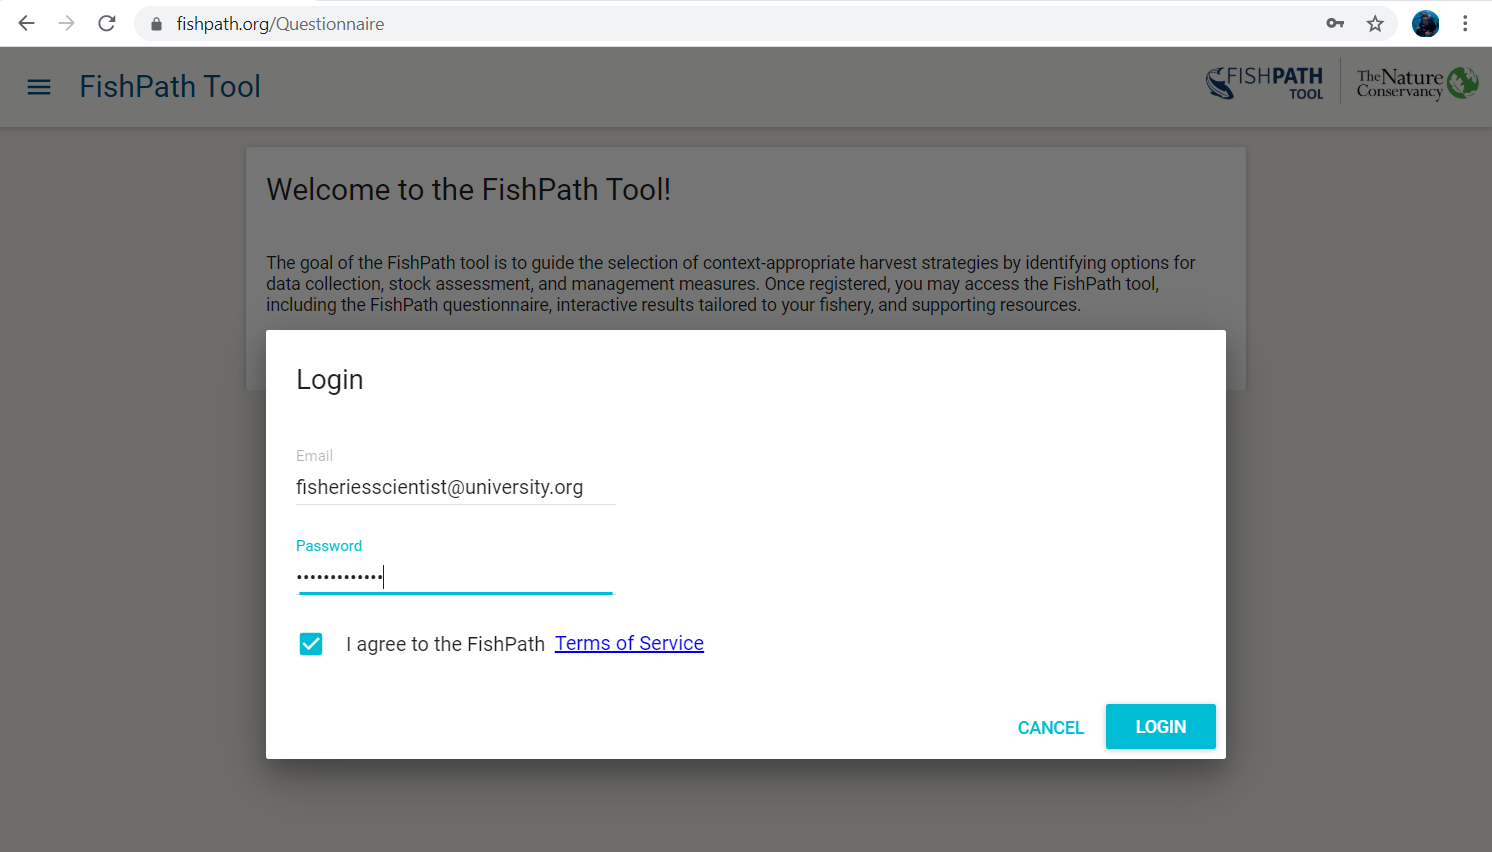
\includegraphics[width=0.95\linewidth]{images/login-page} 

}

\caption{Login Page of the FishPath Tool.}\label{fig:login-page}
\end{figure}

\hypertarget{fishpath-tool-dashboard}{%
\section{FishPath Tool Dashboard}\label{fishpath-tool-dashboard}}

After creating an account (new user) or logging in (existing user), the user is directed to the FishPath Tool Dashboard (Figure \ref{fig:dashboard}), or the user's ``homepage'' of the FishPath Tool. On the FishPath Tool Dashboard, users view 4 headings:

\begin{enumerate}
\def\labelenumi{\arabic{enumi}.}
\tightlist
\item
  \textbf{``FishPath Tool User Guide''} (this guide), which contains detail on using the FishPath Tool and interpreting results.
\item
  \textbf{``My Fisheries''}, which provides a list of the user's current list of fisheries they have started or completed in the tool. Users may access their fisheries at any time through this section, and return to in-progress FishPath questionnaires or results pages;
\item
  \textbf{``Reference Materials''}, which provides a list of all options contained in the FishPath Tool with details and reference materials, and the ability to download the Question List;
\item
  \textbf{``Get Support, Ask a Question, or Help us Improve the FishPath Tool''}, which allows the user to send questions or feedback to the FishPath team.
\end{enumerate}

\begin{figure}

{\centering 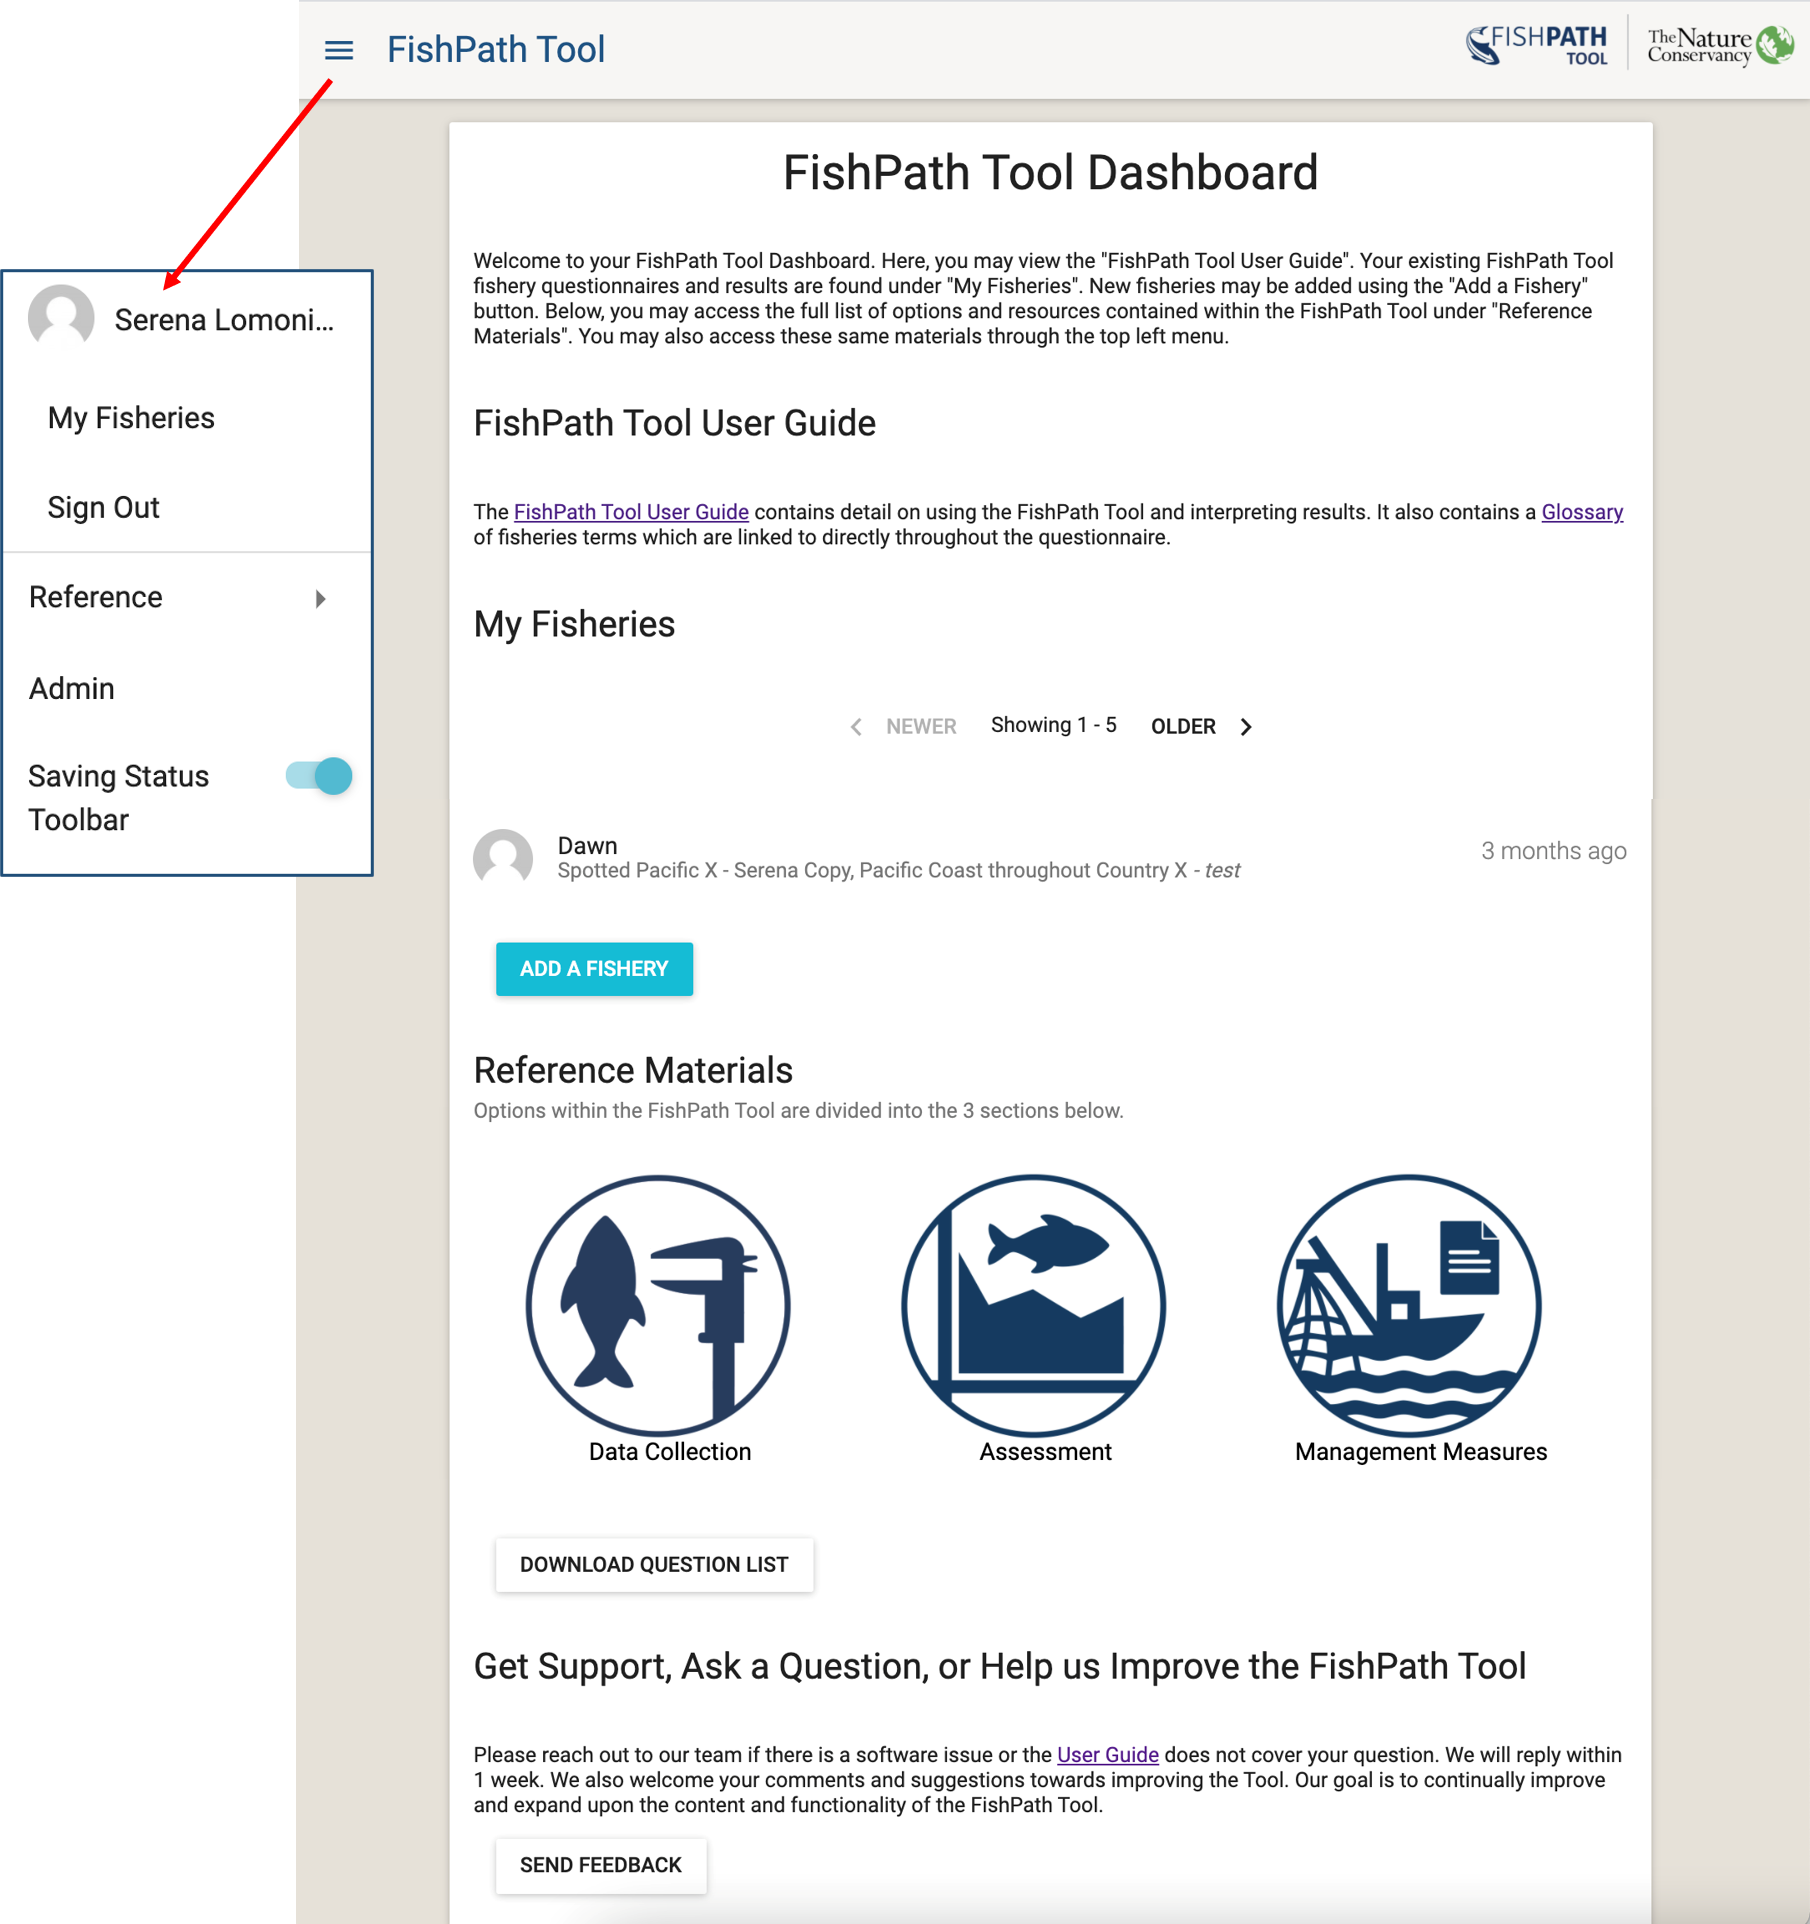
\includegraphics[width=0.95\linewidth]{images/user-dashboard} 

}

\caption{FishPath Tool Dashboard, or the homepage for FishPath Tool users. The pop out shows the FishPath Tool Dashboard drop-down menu.}\label{fig:dashboard}
\end{figure}

\hypertarget{fishpath-tool-side-bar-menu}{%
\subsubsection{FishPath Tool Side Bar Menu}\label{fishpath-tool-side-bar-menu}}

At the top left of the screen, users can view a drop-down side-bar menu by clicking the 3 horizontal lines (Figure \ref{fig:dashboard}). This menu allows users to return to the Dashboard, Sign Out, access reference materials, and toggle functionality called ``Saving Status Toolbar''.

\hypertarget{saving-status-toolbar}{%
\paragraph{Saving Status Toolbar}\label{saving-status-toolbar}}

The ``Saving Status Toolbar'' (Figure \ref{fig:saving-status}) will notify the user of the status of saving questionnaire responses and results. This toolbar appears at the bottom of the Questionnaire and results screens to notify the user if their changes have been saved to the database. If all changes have been fully saved, it will display ``All Changes Saved''. In the event of inconsistent internet, changes may not save to the database immediately and status will be displayed (e.g., ``Offline - 2 pending changes''). The Tool will keep attempting to save everything until successful. Users can continue answering the questionnaire or make other changes while changes are pending. However, users should not close or refresh the browser until all answers have been saved. If the browser is closed or refreshed before the save is complete, then those changes will be lost. The user will be notified that changes will be lost before closing or refreshing the page. For more information on using the tool in settings of intermittent internet connectivity, please see \protect\hyperlink{faq-internet}{this FAQ below}.

\begin{figure}

{\centering 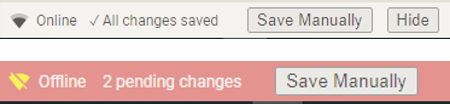
\includegraphics[width=0.95\linewidth]{images/saving-status-toolbar} 

}

\caption{Saving Status Toolbar functionality. The top image shows saved; the bottom image shows changes pending.}\label{fig:saving-status}
\end{figure}

\hypertarget{adding-a-new-fishery}{%
\section{Adding a New Fishery}\label{adding-a-new-fishery}}

Selecting the blue button ``Add a Fishery'' allows users to start a new fishery in the FishPath Tool that will be added to their account. A pop-up ``Fishery Information'' screen appears to prompt users to define the fishery of focus (Figure \ref{fig:fishery-info}), using the fields below. This information helps users define the fishery to which they will be applying FishPath, so that answers will be directed at that fishery only. It is also used by TNC to better understand the use of the FishPath Tool and provide high-level aggregate information about fishery characteristics.

All fisheries and information saved in the Fishpath Tool (including questionnaire responses, notes, and results) are only accessible by the submitting user and FishPath Tool Admins. If desired, users may choose to \protect\hyperlink{Results-Actions}{\textbf{share fishery results}}.

\begin{itemize}
\tightlist
\item
  Fishery Common Name(s):
\item
  Genus species:
\item
  Fleet and Gear Type(s):
\item
  Country (may select multiple):
\item
  Geographic Area of the Fishery:
\item
  In which of these 3 contexts is the FishPath Tool being used for this fishery? This information is collected to better understand Tool use patterns.

  \begin{itemize}
  \tightlist
  \item
    Exploratory test run\\
  \item
    Facilitated workshop for specific fishery
  \item
    Individual use for specific fishery
  \end{itemize}
\end{itemize}

\begin{figure}

{\centering 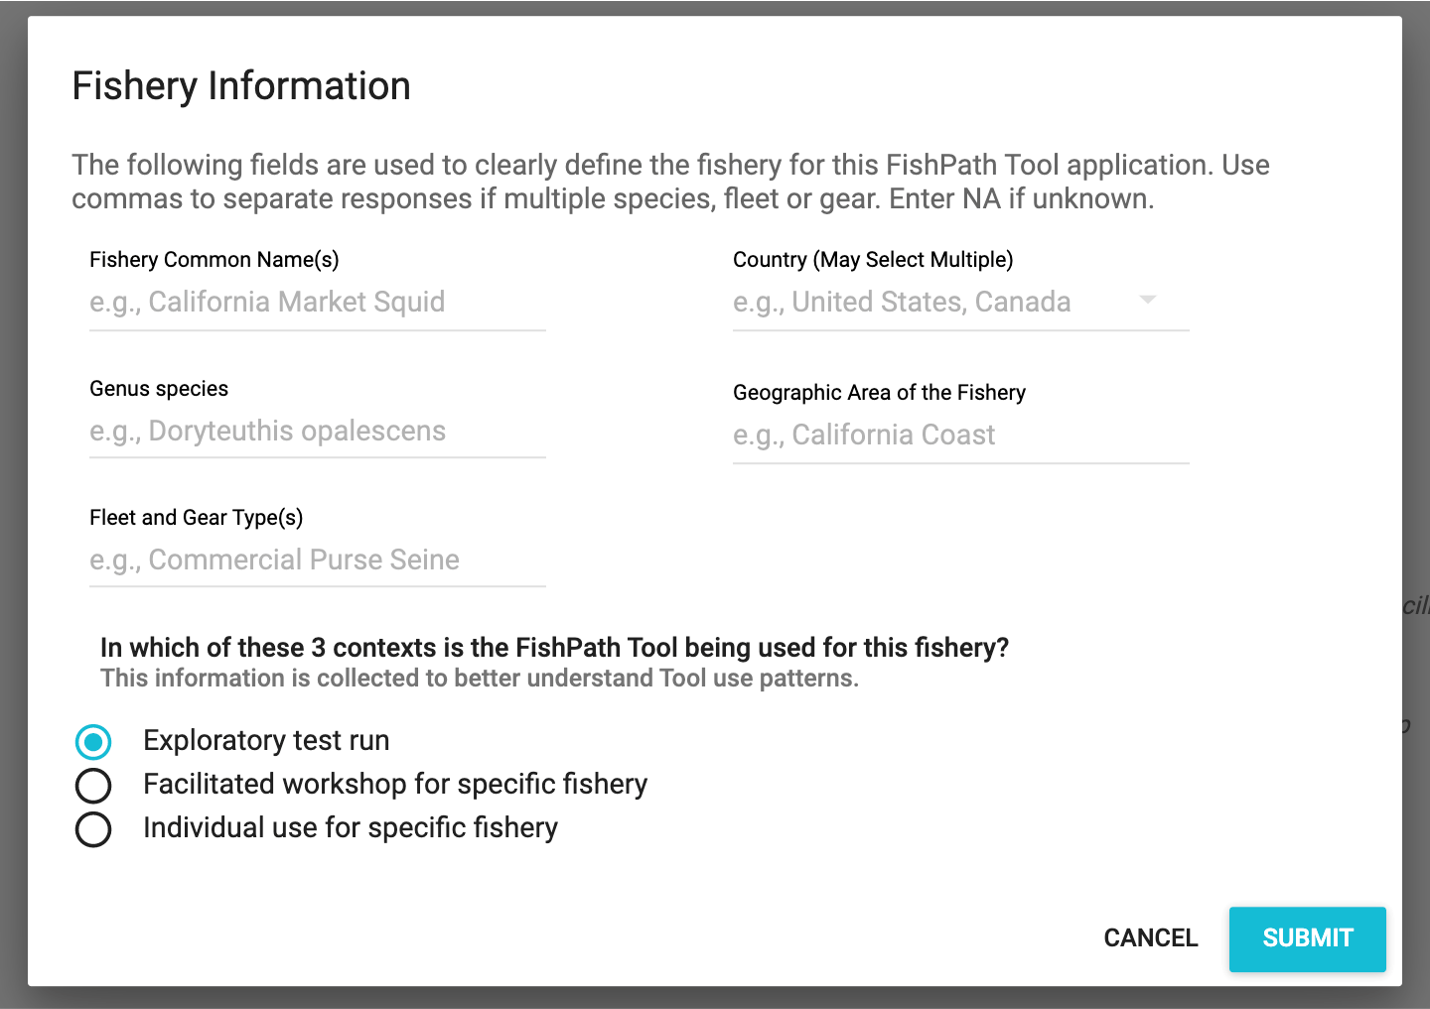
\includegraphics[width=0.95\linewidth]{images/fishery-info-screen} 

}

\caption{Fishery Information pop-up screen of the FishPath Tool.}\label{fig:fishery-info}
\end{figure}

Upon selecting ``Submit'', the user is prompted to select one of the 3 harvest strategy components (sections) of the FishPath Tool (Data Collection, Assessment, Management Measures) and begin the FishPath tool questionnaire (Figure \ref{fig:fishery-entry}). Users can complete and review results from these sections independently and in any order. A pencil in the upper-right corner allows users to edit the fishery information (input in Figure \ref{fig:fishery-entry}) at any time.

\begin{figure}

{\centering 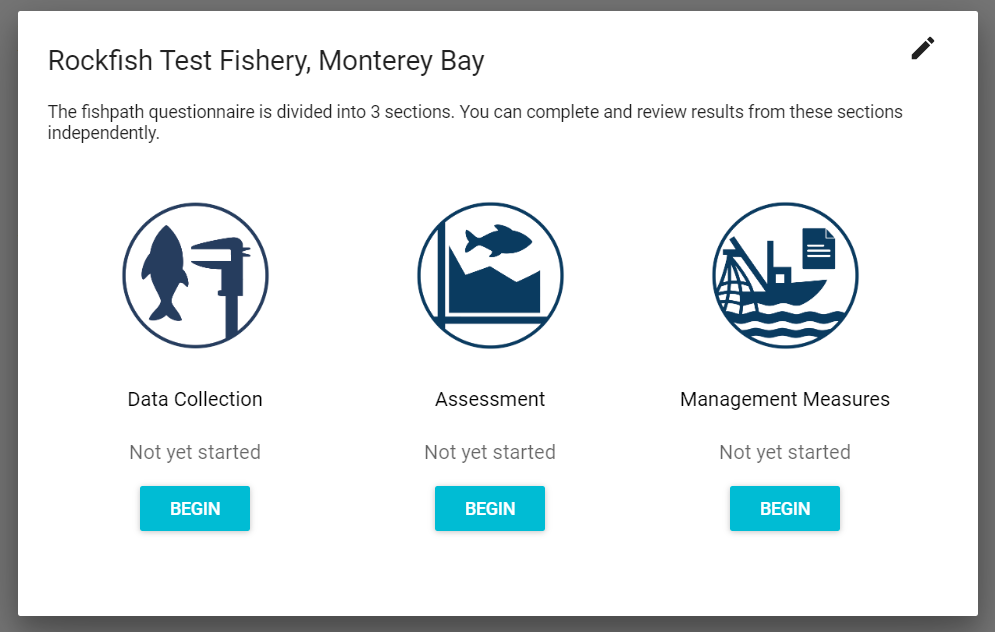
\includegraphics[width=0.95\linewidth]{images/fishery-entry-screen} 

}

\caption{Entry screen to the FishPath Tool questionnaire after fishery information has been defined. The pencil icon (red arrow) allows users to edit fishery name and details.}\label{fig:fishery-entry}
\end{figure}

\hypertarget{fishpath-tool-questionnaire}{%
\chapter{FishPath Tool Questionnaire}\label{fishpath-tool-questionnaire}}

The goal of the FishPath Tool questionnaire is to elicit information about all aspects of the fishery. This information leads to the activation of assumptions, cautions and considerations for each option. Across the three sections (Data Collection, Assessment, and Management Measures) the user answers a series of \textasciitilde120 questions. Questions are categorized in 6 categories, which indicate the nature of the information in the question:

\begin{enumerate}
\def\labelenumi{\arabic{enumi}.}
\tightlist
\item
  Biology/Life History
\item
  Data Availability
\item
  Governance
\item
  Management
\item
  Operational Characteristics
\item
  Socio-Economic
\end{enumerate}

Some questions are relevant to multiple sections (Data Collection, Assessment, Management Measures). Once answered, these will not appear in any subsequent section in which they occur. For more information on how questions that cross multiple sections are displayed, please see \protect\hyperlink{faq-question-numbering}{this FAQ below}.

At any time, the user may close and later return to their session via their ``My Fisheries'' dashboard. Once the user has completed an individual section, the user may either complete a subsequent section or view results from the completed section. Results for any section become available once the user has completed the respective questionnaire section.

After viewing the entry screen to the FishPath questionnaire (Figure \ref{fig:fishery-entry}), the user selects one of the 3 sections. An overview screen will appear with the name of the section, the number of questions associated with that section, and a short guidance on answering the questions (Figure \ref{fig:dc-overview}). The user can then choose to ``Begin'' the section or ``Choose Another Section''.

\begin{figure}

{\centering 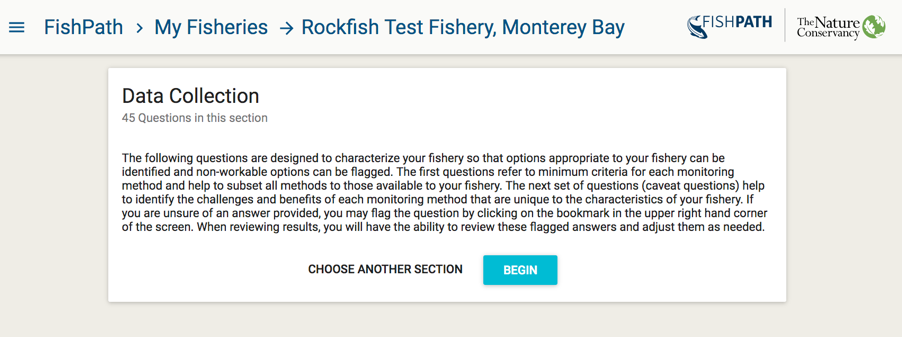
\includegraphics[width=0.95\linewidth]{images/dc-overview} 

}

\caption{Data Collection section overview.}\label{fig:dc-overview}
\end{figure}

\hypertarget{anatomy-of-a-fishpath-tool-question}{%
\section{Anatomy of a FishPath Tool Question}\label{anatomy-of-a-fishpath-tool-question}}

Figures \ref{fig:question-anatomy} and \ref{fig:bookmark-notes} show examples of the FishPath Tool question screen.

\begin{figure}
 
 {\centering 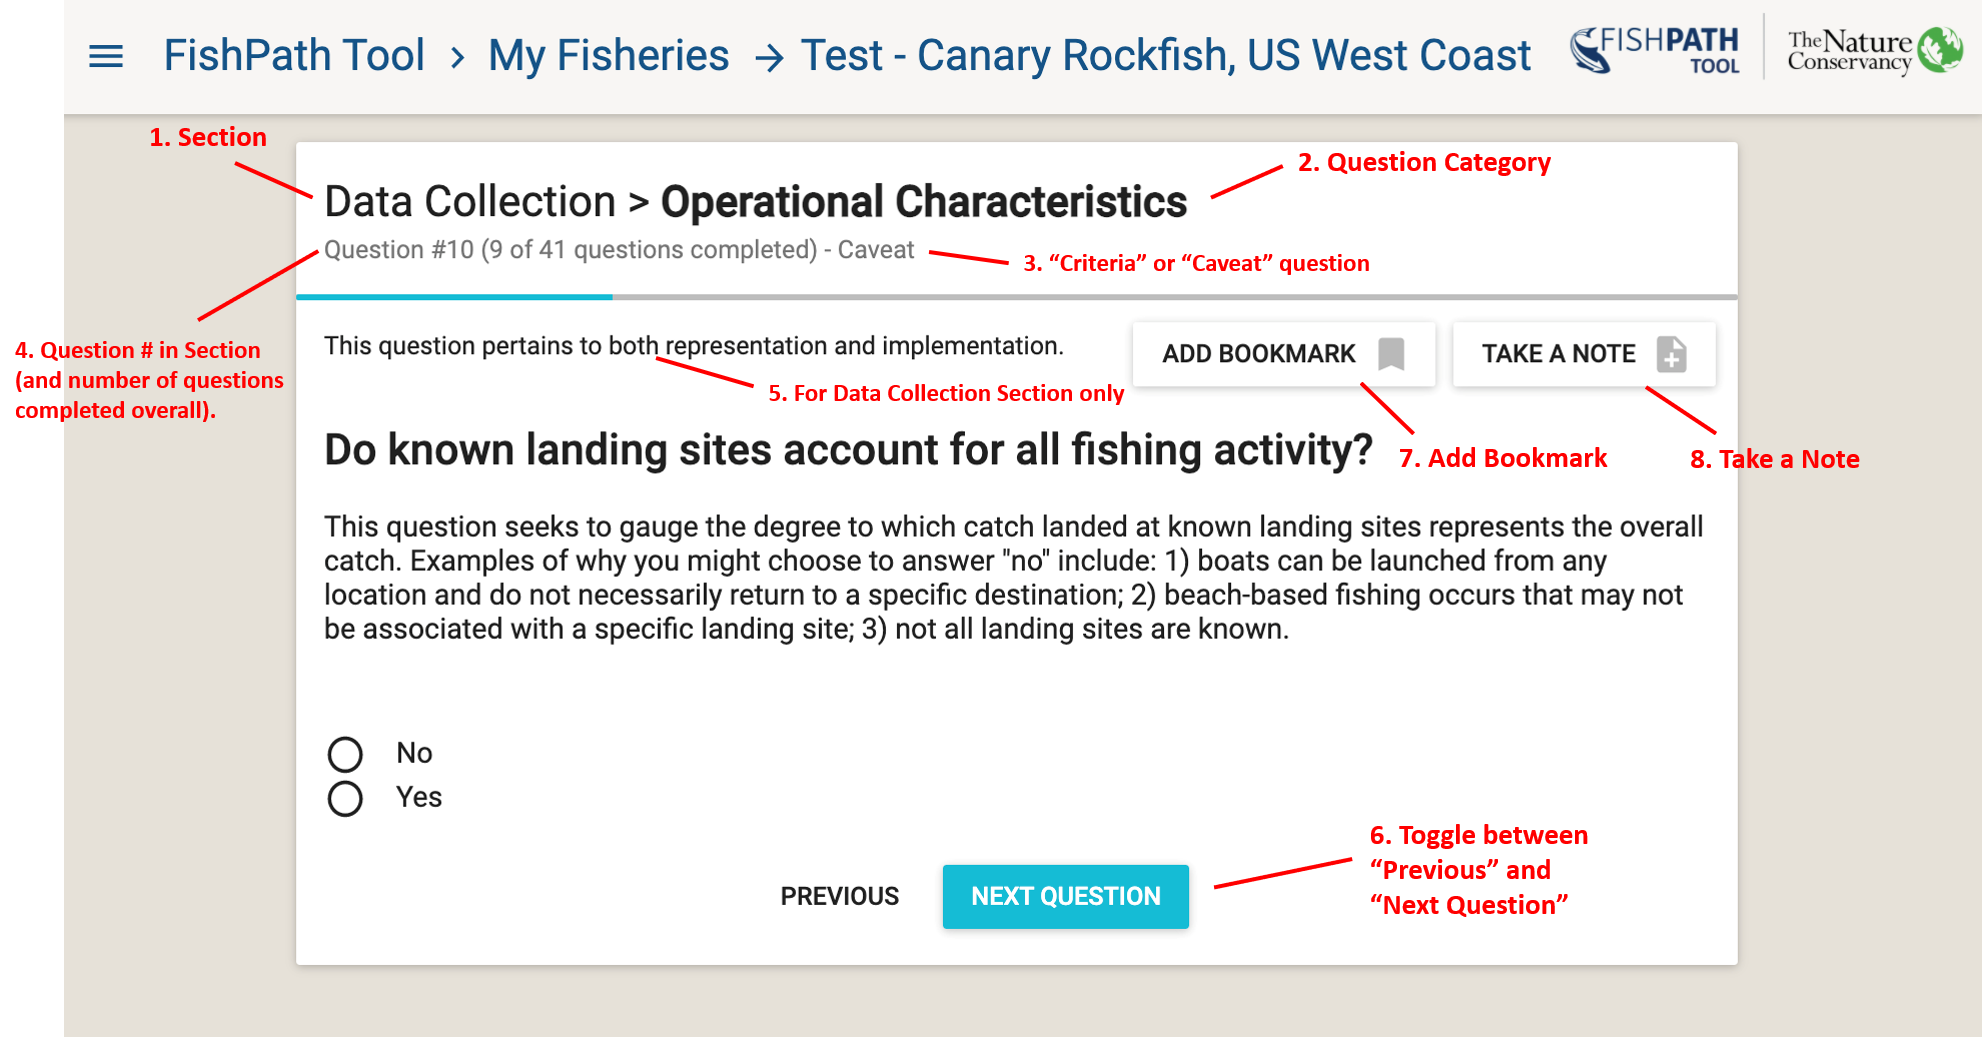
\includegraphics[width=0.95\linewidth]{images/question-anatomy} 
 
 }
 
 \caption{Anatomy of a FishPath Tool question.}\label{fig:question-anatomy}
 \end{figure}

\begin{enumerate}
\def\labelenumi{\arabic{enumi}.}
\tightlist
\item
  At the top of the screen, the \textbf{section} is shown (either Data Collection, Assessments, or Management Measures).
\item
  The section is followed by the \textbf{question category} (i.e., Biology/Life History, Data Availability, Governance, Management, Operational Characteristics, or Socio-Economic).
\item
  A sub-heading identifies whether the question is a \textbf{``criteria'' or a ``caveat''} question.
\item
  The sub-heading also indicates the \textbf{number of questions answered} and remaining within that section.
\item
  For the Data Collection section only: This notifies users whether the question has ramifications for the ability to collect representative data, or pertains to the ability to implement a data collection program, or both. It is simply intended to help the user better understand and answer the question.
\item
  Toggle between \textbf{``Previous''} and \textbf{``Next Question''}. At the bottom of the screen, the user may advance to the next question or return to the previous question.
\item
  There is the ability to \textbf{``Bookmark''} the question. A bookmark flags questions for ease of later revisiting (Figure \ref{fig:bookmark-notes}). A question may be bookmarked for reasons such as if the answer is unknown, it needs further consideration or input, is in dispute, or if the user feels the question is critical. As all questions must be answered in order to review results, adding a bookmark allows users to provide an interim response that may be revisited in the results section, once the user can evaluate the relative impact of their response.
\item
  Users can \textbf{``Take A Note''} on a question (Figure \ref{fig:bookmark-notes}). Notes can be taken for a variety of reasons such as to clarify why a certain response was given, to capture important discussion about a question, why the question was bookmarked or noting a response requiring further research. Notes can later form an important part of draft harvest strategy development, and, by providing justification for the response, can maintain traceability and replicability. When connected to the internet, all notes made will be saved into the FishPath Tool and available to the user for reference.
\end{enumerate}

\begin{figure}
 
 {\centering 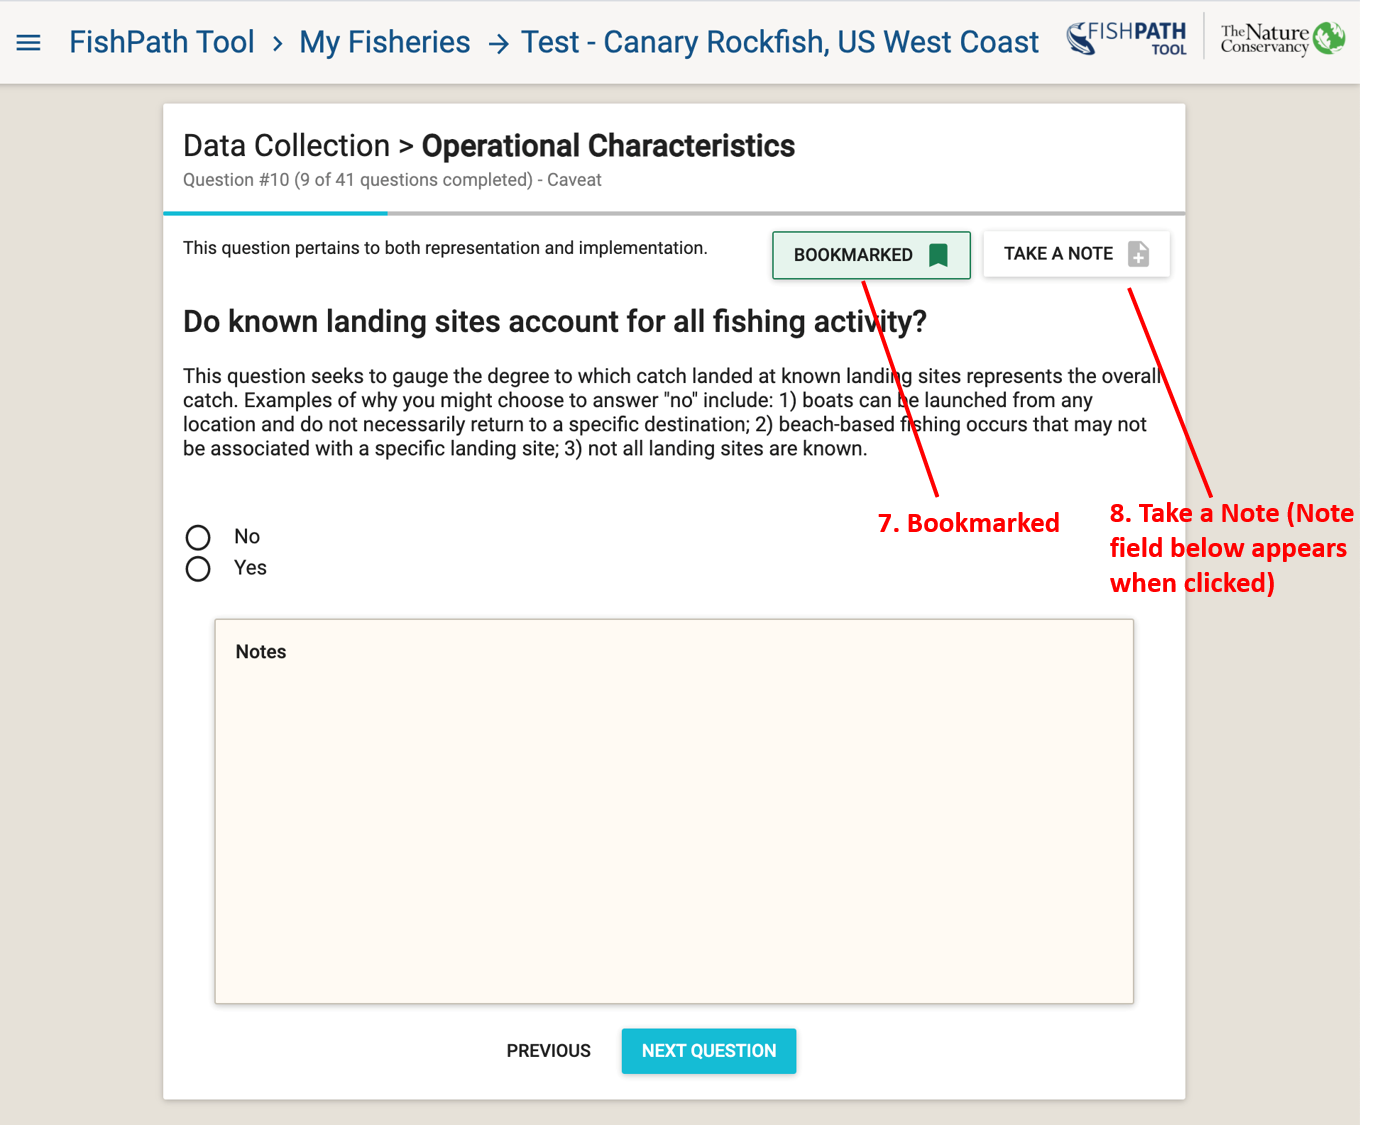
\includegraphics[width=0.95\linewidth]{images/bookmark-notes} 
 
 }
 
 \caption{Example FishPath Tool question with “Bookmark” (green) and “Take a note” (text box) functionality selected.}\label{fig:bookmark-notes}
 \end{figure}

\hypertarget{criteria-and-caveat-questions}{%
\section{Criteria and Caveat Questions}\label{criteria-and-caveat-questions}}

Questions are designated as either ``Criteria'' or ``Caveats'' or both, which refers to how question responses are linked to options contained within the FishPath Tool.

A Criterion question is used to determine whether the fishery meets a minimum qualification required to apply an option. Questions whose responses invoke ``caveats'' will not eliminate options, but rather invoke traffic light-colored warnings (red, yellow, orange), or positive attributes (green), against specific options.

\hypertarget{subjective-questions}{%
\section{Subjective Questions}\label{subjective-questions}}

While the majority of questions within the FishPath Tool are intended to be answered definitively (objective), certain questions are subjective in nature. For example, a subjective question may ask to rank certain fishery characteristics on a qualitative scale (e.g., ``low'', ``moderate'', ``high''). This subjective design is intentional, as it allows users to think through key, relative characteristics of their fishery that will influence the feasibility of implementing certain management options.

Generally, the best approach to take when completing the questionnaire is to aim to do so relatively efficiently, without overly laboring or debating over any one question. If in doubt, the question can be bookmarked, and notes can be taken, for easy revisiting later. The transparency of the FishPath Tool allows users to explicitly see how their response to any one question influences the results (by invoking criteria or caveats), and to \protect\hyperlink{bookmarked-questions-and-influential-answers}{\textbf{readily change their answer if desired}}. Moreover, the aim of the questionnaire is to obtain an overall profile of the fishery's characteristics to best inform the choice of harvest strategy option. As such, questions may pertain to only a few options, or they may not invoke strong caveats. The goal is to appraise the fishery as a whole, as opposed to focusing on any single question.

\hypertarget{completing-the-questionnaire}{%
\section{Completing the Questionnaire}\label{completing-the-questionnaire}}

Upon completing or exiting any of the three sections, a pop-up summary window appears with the questionnaire status (Figure \ref{fig:summary-screen}). Users may review their results for completed sections, or otherwise continue the questionnaire.

The questionnaire is periodically updated by the FishPath team to reflect the latest fisheries science. If there are any new or outstanding questions, the section will no longer display as ``Complete'' in the pop-up summary window (Figure \ref{fig:summary-screen}) when returning to a fishery questionnaire. Instead, the number of new questions needing to be answered will be displayed (e.g., ``45 of 46 questions answered''). For more information on questionnaire updates, please see \protect\hyperlink{faq-content-updates}{this FAQ below}.

\begin{figure}
 
 {\centering 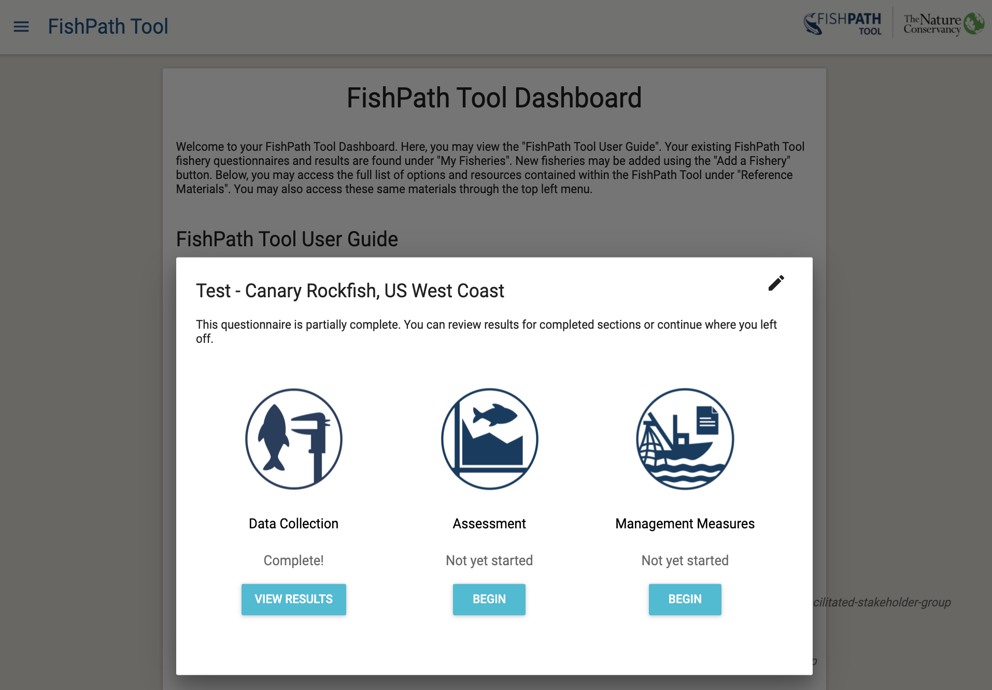
\includegraphics[width=0.95\linewidth]{images/summary-screen} 
 
 }
 
 \caption{Summary window of the 3 FishPath Tool questionnaire sections, showing questionnaire progress.}\label{fig:summary-screen}
 \end{figure}

\hypertarget{fishpath-tool-conceptual-framework}{%
\section{FishPath Tool Conceptual Framework}\label{fishpath-tool-conceptual-framework}}

At a high level, the FishPath Tool is a framework that ``matches'' the user's questionnaire responses with the 150+ options contained within the Tool (Figure \ref{fig:conceptual}). In other words, the user's answers to the questions help characterize the fishery. Each answer is used to flag considerations when applying a given option to the fishery. These considerations (and types of questions) may take two forms. Criteria denote that the fishery does or does not meet the basic requirements to undertake an option. Alternatively, caveats are warnings to consider when applying the option. Caveats may either be scaled intensity warnings denoted by traffic light colors, or static caveats which always apply to the option.

\begin{figure}
 
 {\centering 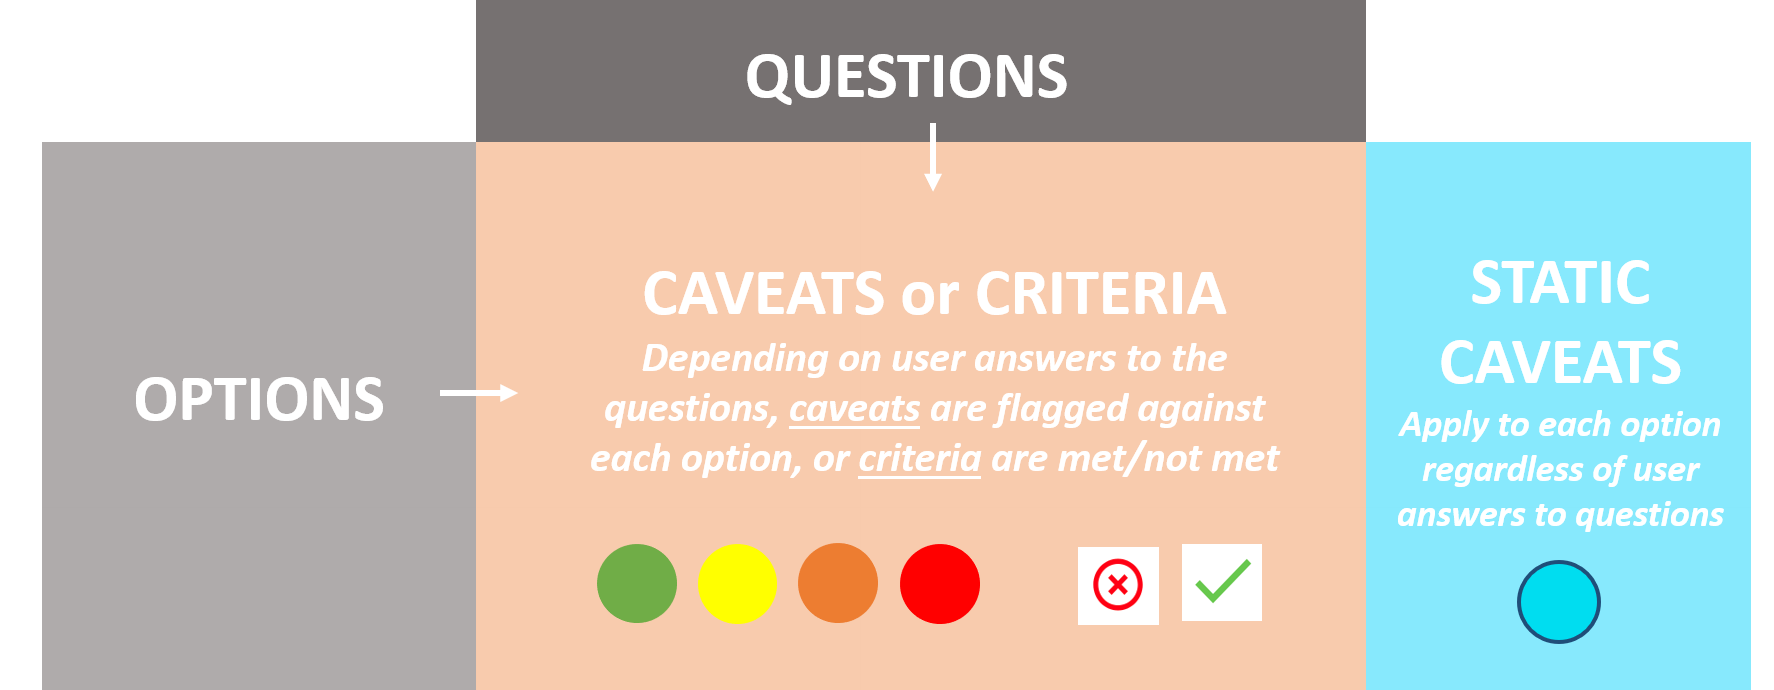
\includegraphics[width=0.95\linewidth]{images/conceptual-framework} 
 
 }
 
 \caption{High level, conceptual framework of the FishPath Tool, demonstrating the linkages between questions, options, and criteria or caveats.}\label{fig:conceptual}
 \end{figure}

\hypertarget{fishpath-tool-framework-overview-of-the-3-sections}{%
\subsection{FishPath Tool: Framework Overview of the 3 Sections}\label{fishpath-tool-framework-overview-of-the-3-sections}}

\hypertarget{data-collection-section}{%
\subsubsection{Data Collection Section}\label{data-collection-section}}

The Data Collection section of the FishPath Tool aims to support the user in understanding which broad categories of information to collect, as well as the data collection mechanisms that are best suited for the fishery context, capacity, and realities of on-the-ground implementation.

There are a range of data collection mechanism options (from market surveys, to logbooks and observer programs) in the FishPath Tool. These options are subdivided according to the broad category of information that may be collected, as these influence the viability of the data collection option. The \protect\hyperlink{data-categories}{\textbf{four data categories}} in the FishPath tool are: 1) data that yield a basic understanding of the fishery; 2) biological information; 3) data that can inform temporal trend analyses (data time series), and 4) data that are of a sufficient quality to inform a model-based stock assessment.

\hypertarget{assessment-section}{%
\subsubsection{Assessment Section}\label{assessment-section}}

The Assessment section of the FishPath Tool allows the user to understand which data-limited stock assessment approaches are available and best suited to their fishery. In the FishPath Tool, an assessment is defined as any analysis or performance indicator that gives useful information for management by direct or indirect measures of stock status. This could range from a ``cause for concern'' arising from expert judgement, qualitative risk assessments, values of empirical indicators relative to pre-defined trigger levels, multiple indicator frameworks, to life history analyses that provide estimates of fishing mortality, (F), or fishing mortality at maximum sustainable yield, (FMSY), catch-only models, size or length based approaches, to population dynamics model-fitting approaches that estimate biomass.

Based on the fishery characteristics and the quality and type of available data (elicited from the questionnaire), user responses flag caveats and raise criteria against the \protect\hyperlink{assessment-categories}{\textbf{assessment options}}.

\hypertarget{management-measure-section}{%
\subsubsection{Management Measure Section}\label{management-measure-section}}

In the FishPath Tool, the Management Measures section allows users to review and refine appropriate options for managing fishing mortality. \protect\hyperlink{management-measure-categories}{\textbf{Management measure options}} within the FishPath Tool can take many forms including spatial, temporal, effort, catch, and gear related restrictions. The FishPath Tool does not have any minimum criteria listed for management measures, but instead uses cautionary caveats. Multiple management measures can and should be used together. The FishPath Tool results do not prescribe or give guidance on the specific form of the harvest rule, nor the strength of adjustment in response to assessment outcomes. However, the FishPath Tool does direct users to resources and tools that can support this process, located within the description of each option.

\hypertarget{fishpath-tool-interactive-results-page}{%
\chapter{FishPath Tool Interactive Results Page}\label{fishpath-tool-interactive-results-page}}

The FishPath Tool Interactive Results Pages allow users to view and interact with all of the options contained within FishPath and understand how each option may apply to their fishery.

Upon completion of the questionnaire for any section, the user is directed to the FishPath Tool Interactive Results page (Figure \ref{fig:results-overview}). The results are presented separately for each of the 3 sections, or harvest strategy component: 1) Data Collection; 2) Assessment; and 3) Management Measures (Figure \ref{fig:results-overview}, see arrow).

Each of the three sections of the results can be accessed individually without needing to complete all three sections. If a user has not completed the questionnaire in at least one of the sections, they will be prompted to return to finish the section questionnaire before accessing results (Figure \ref{fig:summary-screen}).

In this section, users should first begin with the process to ``Narrow your Results'' (Figure \ref{fig:results-overview}, blue button). Below, the layout and functionality of this screen is explained, followed by steps in the results narrowing process.

\begin{figure}

{\centering 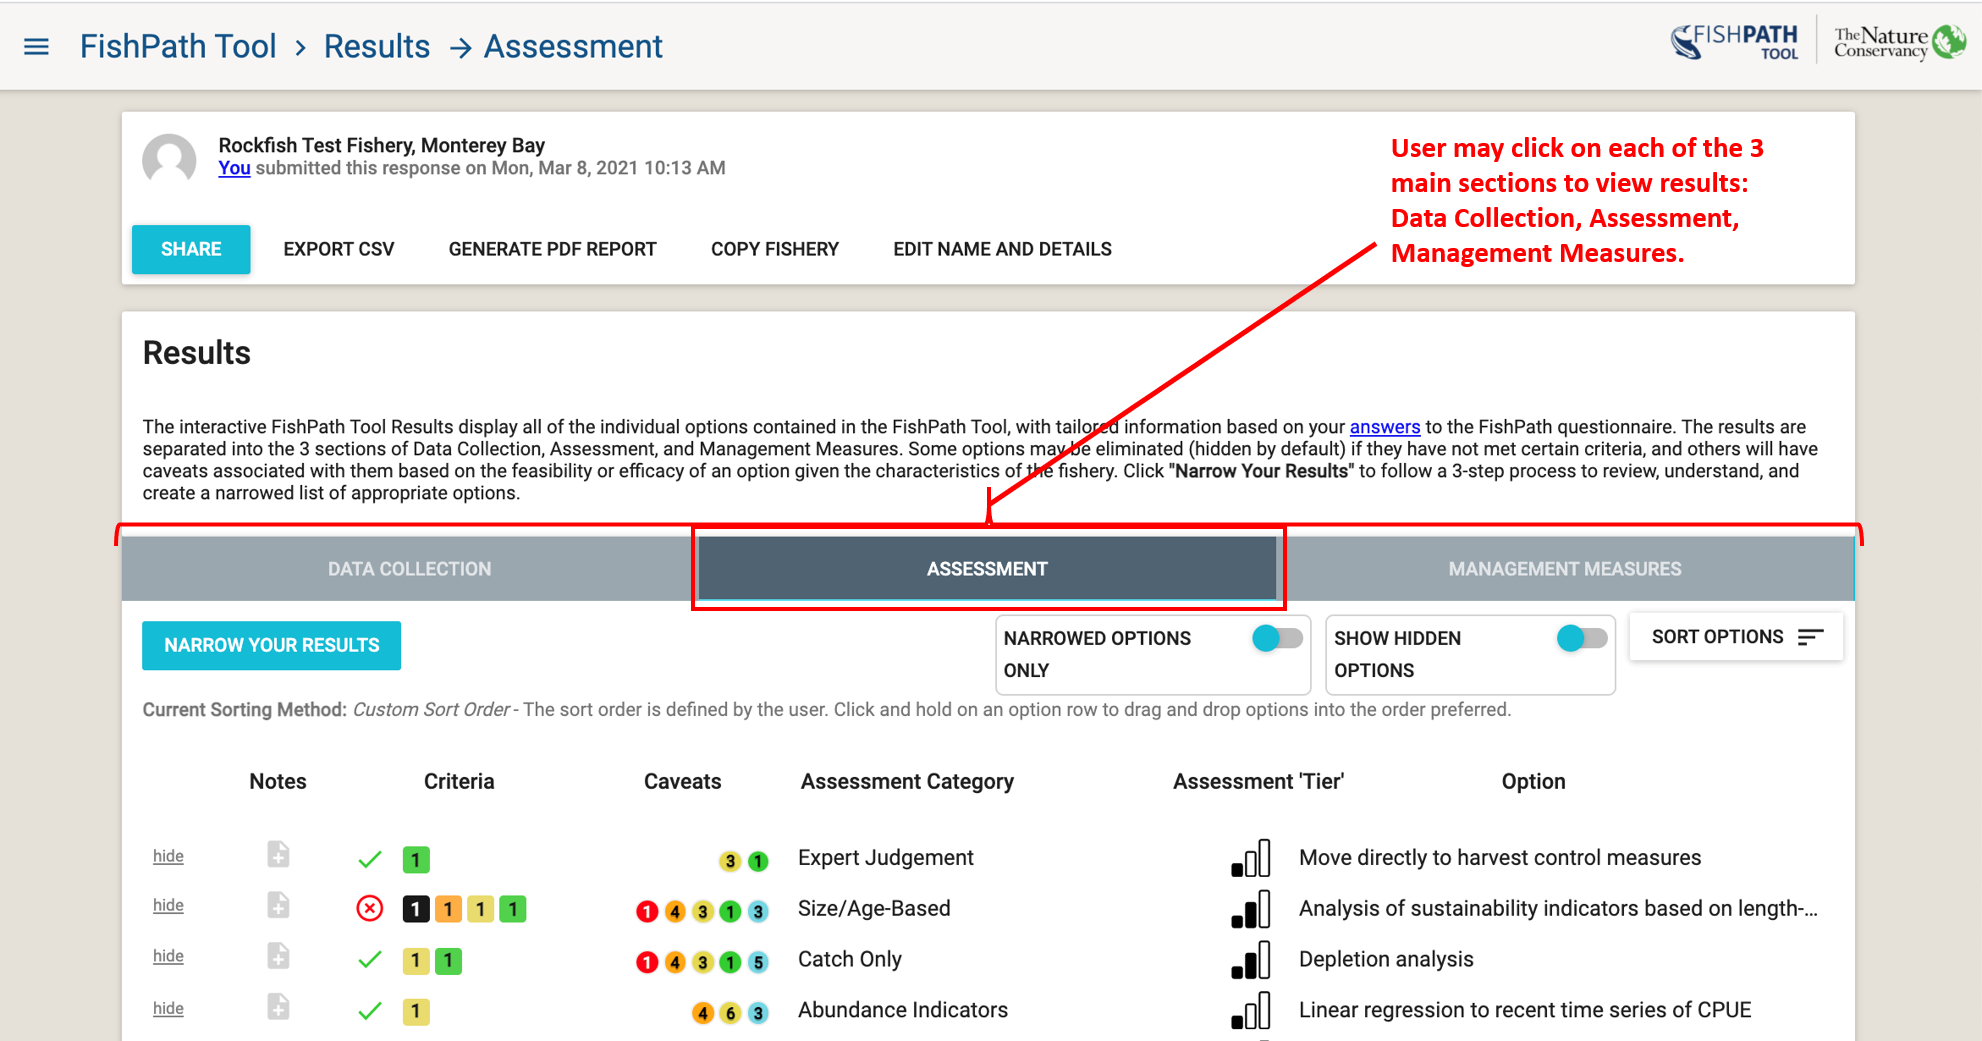
\includegraphics[width=0.95\linewidth]{images/results-overview} 

}

\caption{Initial results display screen in the FishPath Tool (featuring the Assessment section in the red box), displaying a snapshot of results, not a full listing.}\label{fig:results-overview}
\end{figure}

Figure \ref{fig:results-components} shows the general components of the results page. Each of these is elaborated below:

\begin{enumerate}
\def\labelenumi{\arabic{enumi}.}
\tightlist
\item
  \protect\hyperlink{interactive-results-table}{Interactive Results Table}
\item
  \protect\hyperlink{show-hidden-options-and-sort-options}{Show Hidden Options and Sort Options}
\item
  \protect\hyperlink{bookmarked-questions-and-influential-answers}{Bookmarked Questions and Influential Answers}
\item
  \protect\hyperlink{Results-Narrowing}{Results Narrowing Process}
\item
  \protect\hyperlink{Results-Actions}{Actions to Share Results and Edit Fishery Info}
\item
  \protect\hyperlink{view-only-mode-shared-fishery}{View-Only Mode (Shared Fishery)}
\end{enumerate}

\begin{figure}

{\centering 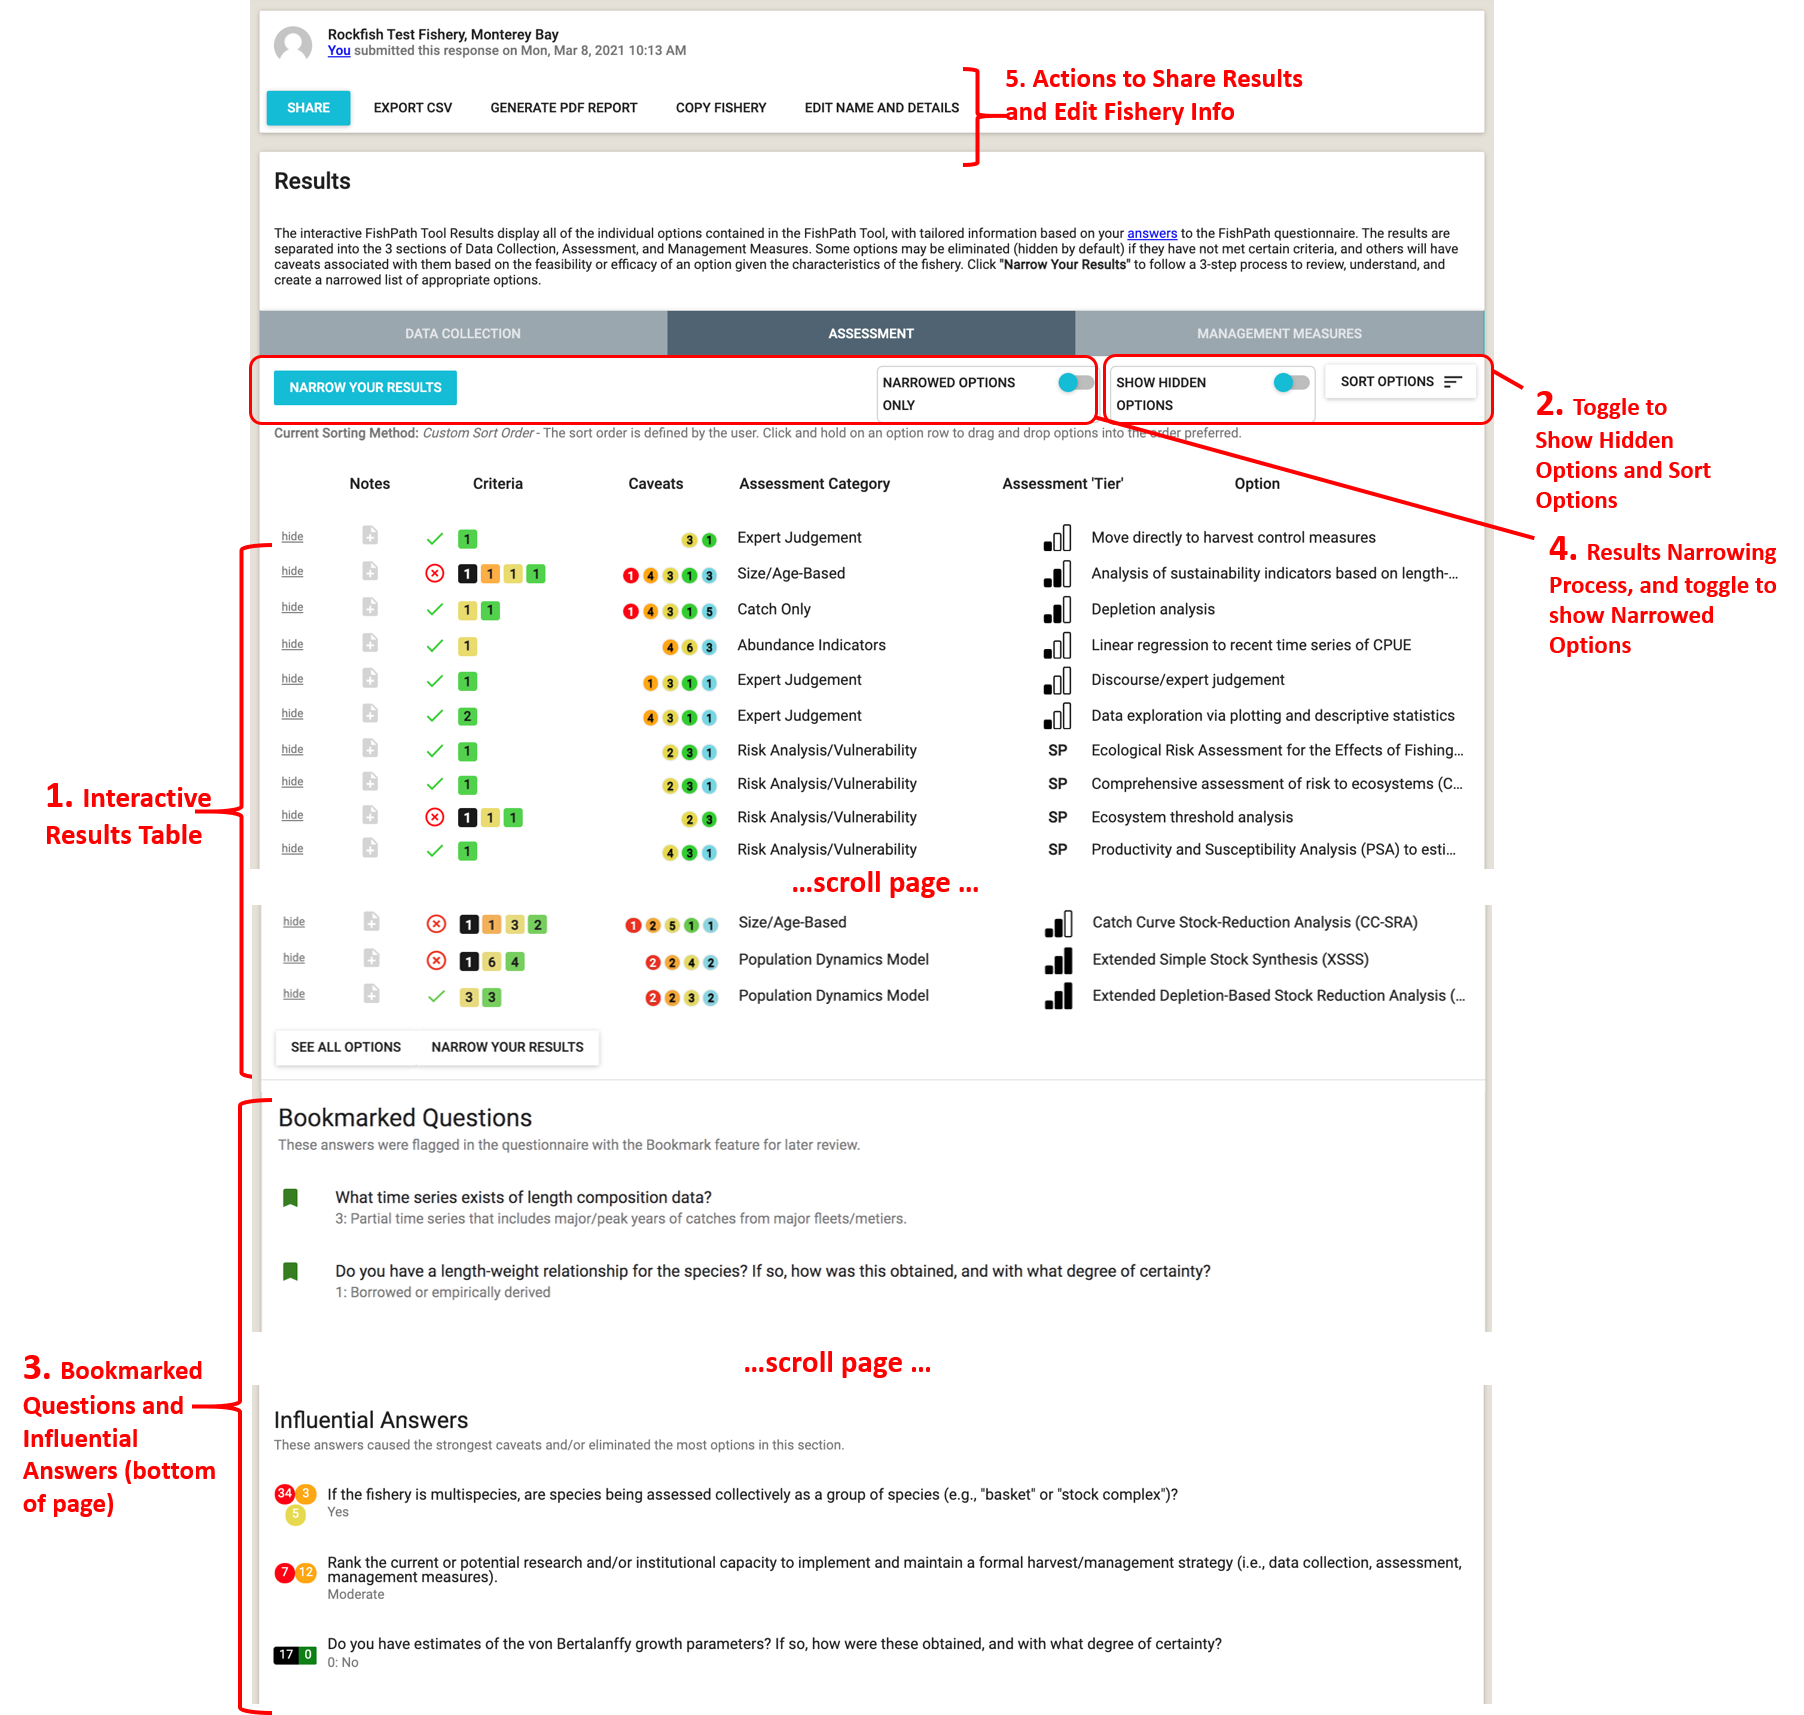
\includegraphics[width=0.95\linewidth]{images/results-components} 

}

\caption{Key components (red labels 1-5) of the FishPath Interactive Tool Results Page.}\label{fig:results-components}
\end{figure}

\hypertarget{interactive-results-table}{%
\section{Interactive Results Table}\label{interactive-results-table}}

The results table lists all the available options for the selected section. Each row represents one option (Figure \ref{fig:result-rows}) and summarizes the criteria met and failed, the caveats invoked, and other details. Each option can be selected and expanded to view its description and full caveats and criteria. Each component of the row is explained below.

\begin{figure}

{\centering 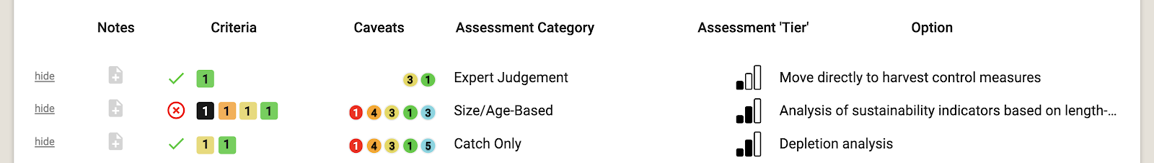
\includegraphics[width=0.95\linewidth]{images/results-rows} 

}

\caption{Headings of the FishPath Tool results table (bold black text) and 3 example options (3 rows). This is the Assessment section.}\label{fig:result-rows}
\end{figure}

\hypertarget{table-structure}{%
\subsection{Table Structure}\label{table-structure}}

\begin{itemize}
\tightlist
\item
  \textbf{Hide/Unhide:} Any option for which one or more of its minimum criteria have not been met by the fishery is automatically ``hidden'' (greyed-out) by the FishPath Tool (Figure \ref{fig:hide}). For any option, including those not meeting minimum criteria, users may manually click this link to ``hide'' the option, or click ``unhide'' to reinstate it. Hidden options are only shown when the toggle ``Show Hidden Options'' is on (red label 2 in Figure \ref{fig:results-components})
\end{itemize}

\begin{figure}

{\centering 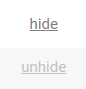
\includegraphics[width=0.1\linewidth]{images/hide} 

}

\caption{Hide, unhide buttons}\label{fig:hide}
\end{figure}

\begin{itemize}
\tightlist
\item
  \textbf{Notes:} As within the questionnaire, notes may be written and saved for each option by clicking on the note icons (Figure \ref{fig:notes}). For example, notes may be taken on fishery-specific details on why that option may or may not be a good fit, or to record the user's or user groups overall evaluation of the option, given its associated criteria and caveats. Alternatively, notes may be taken if options are hidden or reinstated, to justify that choice as documentation. Notes can be included in the PDF report.
\end{itemize}

\begin{figure}

{\centering 
\includegraphics[width=0.15\linewidth]{images/notes} 

}

\caption{Top icon shows an option with a note already taken. Click to view or edit the note. The bottom icon signifies that no note has been taken for the option. Click to create a new note.}\label{fig:notes}
\end{figure}

\begin{itemize}
\item
  \textbf{Criteria (Data Collection and Assessment sections only):} The criteria column provides information on whether the fishery meets the minimum conditions required to undertake the option. If the fishery has met all of the minimum criteria required for an option, a green check is displayed. On the other hand, if a fishery has not met one or more of the minimum criteria required for an option, it is considered to be eliminated, a red X is displayed, and the option is automatically ``hidden''.

  In the Data Collection section, criteria are either ``Not Met''or ``Met'' (Figure \ref{fig:dc-criteria}). In an eliminated option row, black boxes indicate the number of minimum criteria that were not met. Green boxes indicate the number of criteria that were met.
\end{itemize}

\begin{figure}

{\centering 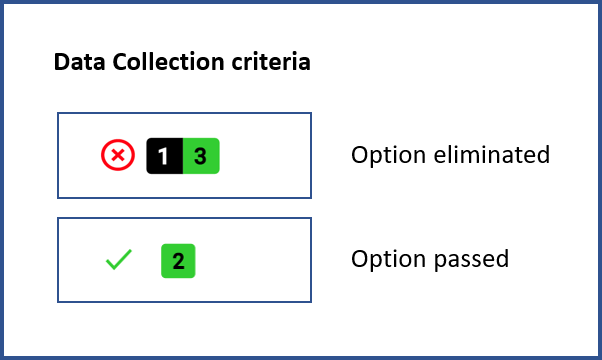
\includegraphics[width=0.35\linewidth]{images/dc-criteria} 

}

\caption{Example of data collection criteria icons. The top row shows an option that has been eliminated, signified by the red X. It was eliminated due to 1 of the 4 criteria not meeting the minimum requirement. The bottom row shows an option that passed, signified by the green check. The option met both of its criteria requirements.}\label{fig:dc-criteria}
\end{figure}

In the Assessment section, criteria are also either ``Not Met'' or ``Met'' (Figure \ref{fig:a-criteria}). In addition, the ``Met'' criteria have ``traffic light'' colors (red, orange, yellow, green) associated with them. The colors represent the quality of each data type and encourage FishPath users to explicitly consider the uncertainty associated with using this data in assessments. For example, say there is a time series of removals for the fishery, but it is missing the removal data from an important fleet. The answer for this question will reflect this bias. Then in the assessment results, options requiring a time series of removals (of any quality) will display that this criterion was met, but it will be colored orange to signify that there is high uncertainty in the removal data. This is a reminder that the user needs to be aware of this uncertainty when performing the assessment and interpreting the results.

The number of ``Not Met'' criteria for each option is shown in the black box, while ``Met'' criteria corresponding to each color of uncertainty levels are shown in the colored boxes. In other words, the number in the black box represents the number of criteria that are ``Not Met'', while summing the numbers within each colored box equal the total number of criteria that have been ``Met''.

\begin{figure}

{\centering 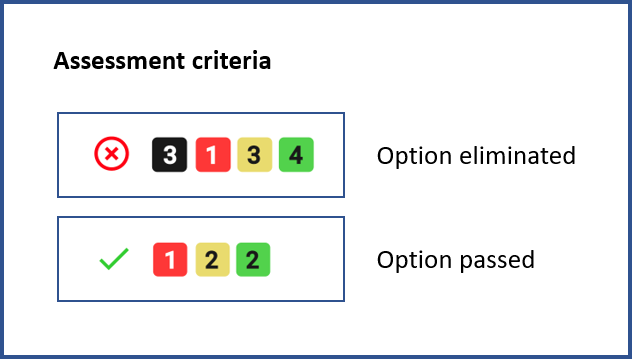
\includegraphics[width=0.35\linewidth]{images/a-criteria} 

}

\caption{Example assessment criteria icons. The top row shows an option that has been eliminated due to 3 criteria that did not meet the minimum requirement. These failed criteria are signified by the 3 in the black box. The bottom row shows an option that has passed criteria, signified by the green check. For both rows, each traffic light color shows the number of passing, or “Met”,  criteria at the various strengths of warning about the data uncertainty.}\label{fig:a-criteria}
\end{figure}

\begin{itemize}
\item
  \textbf{Caveats:} The format of the caveats column is identical across all three sections (Figure \ref{fig:caveats}). Caveats are shown as colored circles with numbers indicating the total number of questionnaire responses that invoked a caveat of that particular color. There are three types of caveats:

  \begin{enumerate}
  \def\labelenumi{\arabic{enumi}.}
  \tightlist
  \item
    \textbf{Cautionary, or warning caveats:} These are marked as red, orange, and yellow circles with the severity or strength of the caveat corresponding to the color (red being highest). These give cautionary guidance based on an attribute of a fishery. For example, if the user responded that the species of interest is susceptible to barotrauma, this would invoke a red caveat against size limits as a management measure, since the fishing-induced mortality of the released (under- or over-sized) fish would render size limits ineffective.
  \item
    \textbf{Positive attributes:} A green colored caveat provides reasoning for why the option might be well-suited for the fishery on the basis of the questionnaire responses.
  \item
    \textbf{Static caveats:} Light blue colored caveats are static caveats that need to be considered for an option, regardless of the fishery or the questionnaire responses. A static caveat is independent of specific fishery circumstances and as such is always present. These include key assessment assumptions, for example, that the assessment option assumes that fishery selectivity has not changed over time, or that the assessment method cannot explicitly address uncertainty.
  \end{enumerate}
\end{itemize}

\begin{figure}

{\centering 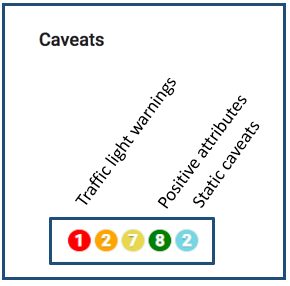
\includegraphics[width=0.35\linewidth]{images/caveats} 

}

\caption{Example of the number of warning caveats (traffic light colors), positive attributes (green), and static caveats (light blue) flagged for an option.}\label{fig:caveats}
\end{figure}

\begin{itemize}
\item
  \textbf{Category:} The Category column allows the user to view the options by categories and is different for each section.

  \begin{itemize}
  \item ~
    \hypertarget{data-categories}{%
    \paragraph{Data Categories}\label{data-categories}}

    In the \textbf{Data Collection Section}, the ``Data Category'' column shows the four categories of data that may be collected.

    \begin{enumerate}
    \def\labelenumi{\alph{enumi}.}
    \tightlist
    \item
      \textbf{Basic understanding of the fishery.} When very little is known about a fishery, stakeholders may want to start by collecting general fishery information or fishery operational characteristics to gain a basic understanding of it. Where very few resources are available, this may be the only available data type, although efforts should be made to move beyond this and make the most efficient use of available capacity. Information collected can be fishery independent or dependent; it can help stakeholders learn more about the size and composition of the fleet, identify the total fished area, determine the gear types used, identify the species landed, make broad estimates regarding catch or fishing effort, and gather other information to aid in better understanding the fishery.
    \item
      \textbf{Temporal trend analyses (data time series).} Data collected for trend analyses are used to track temporal patterns in fishery performance indicators (e.g., catch, fishing effort, catch-per-unit-effort, and catch composition by species), ecosystem indicators, and species biology indicators. In the absence of biomass estimates, temporal trends of other performance indicators can be used for monitoring the health of the fishery over time. Data for trend analyses must be collected at regular, consistent intervals, and must ideally be directly comparable (i.e., collected using the same gear, from approximately the same spatial regions).
    \item
      \textbf{Biological information.} Biological data are collected by obtaining a sample or samples from the species population, recording biometric information (e.g., length/size and weight), gathering information on sex and maturity (e.g., sex identification and maturity identification), and/or collecting biological samples for further study (typically those that are age-related, such as otoliths, scales, and teeth). Biological data provide key information on the species' life history traits, such as growth and reproduction rates. These data are used to better understand the fish stock and to provide the parameters used within fisheries stock assessments and models aiming to estimate the status of the stock.
    \item
      \textbf{To inform model-based stock assessment.} Stock status is estimated via formal (model-based) stock assessments. A stock assessment provides an indicator (or proxy) for the current status of the stock, which can then be compared with a selected reference point. Reference points are the benchmarks used to indicate if the stock is in a desirable or an undesirable state. As opposed to the ``Temporal trend analyses'' category, data collected here inform a quantitative assessment that yields an estimate of biomass or fishing mortality, and the category refers to reliable, detailed data. Data collected to measure the stock status (or proxy) can include reliable time series of catch, fishing effort, catch-per-unit-effort, length compositions, weight compositions, fishery-dependent density, or fishery-independent abundance. Most assessment methods require that any biological sampling undertaken to inform biological parameters should occur prior to, or in conjunction with, data collection efforts to establish reference points.
    \end{enumerate}
  \item ~
    \hypertarget{assessment-categories}{%
    \paragraph{Assessment Categories}\label{assessment-categories}}

    In the \textbf{Assessment Section}, there are two types of categories for each option, the ``\textbf{Assessment Category}'' and ``\textbf{Assessment Output}''.

    \begin{enumerate}
    \def\labelenumi{\arabic{enumi}.}
    \tightlist
    \item
      \textbf{Assessment Category.} Organizes assessment options based on broader families of assessments. This can be related to the main type of input for the options (e.g., Catch Only) or type of assessment option (e.g., Risk Analysis/Vulnerability).

      \begin{enumerate}
      \def\labelenumii{\alph{enumii}.}
      \tightlist
      \item
        \textbf{Abundance Indicators.} Abundance or a proxy for abundance is the main input (e.g., catch-per-unit-effort (CPUE)).
      \item
        \textbf{Catch Only.} A catch history (removals) is the main input. Options might use various life-history parameters, but do not use other time series or size/age based catch information such as length composition or abundance indices.
      \item
        \textbf{General Stock Condition.} General condition of the stock is determined by experts utilizing what information is available, without the use of formal models.
      \item
        \textbf{Life History-Based Methods.} Life history parameters are utilized to determine reference points that can be used to compare to indicators.
      \item
        \textbf{MPA or No-Take Zone/Reserve.} These compare differences between areas inside a no-take zone and outside the no-take zone.
      \item
        \textbf{Multiple Indicators.} Assessment frameworks that formalize management actions to take based on comparisons between multiple indicators and reference points.
      \item
        \textbf{Population Dynamics Model.} Statistically integrated data-driven models underpinned by population dynamics, i.e.~the change in numbers and size and/or age structure over time.
      \item
        \textbf{Risk Analysis/Vulnerability.} Used to determine how at-risk a species or ecosystem is to overfishing or degradation.
      \item
        \textbf{Size/Age-Based.} These options utilize size or age information of the catch, such as the length composition. A time series of catch history is not a requirement for all of these options, but is utilized by some.
      \end{enumerate}
    \item
      \textbf{Assessment Output.} Outputs are units that the assessment option may provide. There are 5 output-based categories. Some assessments may provide multiple outputs.

      \begin{enumerate}
      \def\labelenumii{\alph{enumii}.}
      \tightlist
      \item
        \textbf{Catch Limit.} Catch levels for application in catch-based management to meet management objectives. For example, the catch that corresponds to maximum sustainable yield (MSY).
      \item
        \textbf{Fishing Rate.} Fishing rate for application in effort-based management to meet management objectives. For example, a fishing rate that could be compared to fishing rate at MSY.
      \item
        \textbf{Stock Status.} The relative abundance of the stock.
      \item
        \textbf{Stock Scale.} The absolute abundance of the stock.
      \item
        \textbf{Other Control Rule Metric.} Any indicator other than the four listed above, e.g., changes in species-composition of catches.
      \end{enumerate}
    \end{enumerate}
  \item ~
    \hypertarget{management-measure-categories}{%
    \paragraph{Management Measure Categories}\label{management-measure-categories}}

    In the \textbf{Management Measures Section}, this column is simply titled ``Category'' and displays the categories of management measures. There are 8 categories of management measures.

    \begin{enumerate}
    \def\labelenumi{\alph{enumi}.}
    \tightlist
    \item
      \textbf{Catch Limits.} Catch limits aim to directly manage the fishing mortality of target species by setting a maximum for how many individual, or how much weight of, fish can be removed (including bans) by a fishery in a given time period and/or for specific areas.
    \item
      \textbf{Effort Limits.} Fishing effort limits are aimed at managing fishing mortality by adjusting the fishing activity of fleets to align with a fishing exploitation rate that achieves management objectives. A form of ``input control,'' fishing effort limitations impact all harvested species and not just the target species. Fishing effort limits may be useful in managing multispecies fisheries (where species-specific catch controls may be difficult to implement), in fisheries where gear or fishing effort units are readily controlled, or for fisheries where catch reporting may be unreliable.
    \item
      \textbf{Gear Management.} Gear management specifies the type and design of gear allowed in a fishery, to control the efficiency and harvesting capacity of fishers.
    \item
      \textbf{Temporal Management.} Temporal management regulates harvest by limiting the total number of days or hours per day that a fishery is open. The aim of temporal management is to control the total fishing mortality. This includes fixed rules, or rules that are invoked or modified according to assessment outcomes.
    \item
      \textbf{Spatial Management.} Spatial management involves applying management measures that are spatially explicit, thus specific to one or more areas within the fishery's range. Spatial management may include the use of temporary, rotational, or permanent reserves, spatial closures, or protected areas. It may also include rules that limit individual catch or fishing effort in any one area, requiring fishers to ``move on'' if these limits are exceeded. Spatial harvest control rules can protect areas against the direct and indirect impacts of fishing, thus affecting the entire ecosystem within the restricted areas. Spatial restrictions can be fixed, or they may be invoked or modified within a harvest control rule.
    \item
      \textbf{Size Limits.} Size limits specify the length/size at which species can be legally retained. In the context of a harvest strategy size limits generally aim to protect certain life stages of a species (typically, juveniles and/or mega-spawners), with the goal of increasing productivity, or maintaining sustainability.
    \item
      \textbf{Sex-Specific Regulations.} Sex-specific length/size limits can be implemented for species where males and females mature at different lengths/sizes, whether due to gender differences in growth rate, or age-at-maturity differing by gender. Size regulations can be set separately for each sex to allow maturity to be achieved prior to individuals entering the fishery harvest.
    \item
      \textbf{Other.} This category of management measures includes other options that are not captured by the categories above.
    \end{enumerate}
  \end{itemize}
\item ~
  \hypertarget{assessment-tier-assessments-only}{%
  \paragraph{``Assessment Tier'' (Assessments Only)}\label{assessment-tier-assessments-only}}

  The availability of analytical methods increases as data and biological information increase, and thus more methods typically become available with more information. Some of the simpler approaches may no longer be strong candidates for application in light of more data-driven methods. The ``assessment tier'' category is provided to help determine the general data requirement and model complexity levels for each method. This is especially useful when choosing which methods to prioritize as it allows the user to identify the most data-driven methods rather than attempting to do all possible. A general recommendation is to initially consider or prioritize the highest ``tier'' methods available when choosing methods to implement, though this does not exclude adding other lower tier methods if desired. Indeed, the user is encouraged to consider the trade-offs between research capacity and inherent data uncertainties associated with ``higher tier'' assessment methods, and the lower data requirements and required research capacity, yet reduced robustness, of the ``lower tier'' assessments. In order to emphasize more rigorous methods, ``Stock Prioritization'' and ``Extremely data-poor'' methods are automatically hidden when ``Mid'' or ``High'' options are available.

  There are 5 ``assessment tiers'':

  \begin{enumerate}
  \def\labelenumi{\alph{enumi}.}
  \item
    \textbf{Pre-assessment -- Stock Prioritization (SP):} Methods in this ``tier'' identify species or groups of species that may be classed as ``at risk of harm'', and help prioritize which stocks should be focused on for further management.
  \item
    \textbf{Pre-assessment -- Life-History Based Reference Points (RP):} These methods give target reference points that can then be used in other assessment methods.
  \item
    \textbf{Extremely data-poor (single bar):} Methods that can provide guidance for management if minimal data are available. If mid or high ``tier'' methods are available for the fishery, then the user should preferentially focus on those methods.
  \item
    \textbf{Mid (two bars):} Methods that require a moderate amount of data, usually collected over a series of time. These include methods such as length-based methods, catch-only methods, or multi-indicator frameworks.
  \item
    \textbf{High (three bars):} Methods that, relatively speaking, have the most intensive data and computation requirements, i.e.~population dynamic models.
  \end{enumerate}
\item
  \textbf{Option:} This is the name of the option being considered.
\end{itemize}

\hypertarget{full-option-details}{%
\subsection{Full Option Details}\label{full-option-details}}

Each row in the Results Table displays the option name with summarized results for each option. When users click on any option, a pop-up box appears, which provides full details of the option itself, together with the detail of the criteria and caveats invoked.

First, a description of the option is provided, together with relevant references, and contact information (if available or appropriate). For the Data Collection options, the types of data that may be collected using the option are summarized. For the Assessment section, where available, links to assessment packages are provided.

Next, the invoked criteria and caveats are summarized by (Figure \ref{fig:opt-desc})

\begin{itemize}
\tightlist
\item
  Criteria not met,
\item
  Met criteria,
\item
  Cautionary caveats,
\item
  Positive attribute caveats, and
\item
  Static caveats
\end{itemize}

Next to each, there are individual drop-down menus where the user can find the specific detail on each individual criterion and caveat, along with the question and response that invoked the criterion or caveat.

\begin{figure}

{\centering 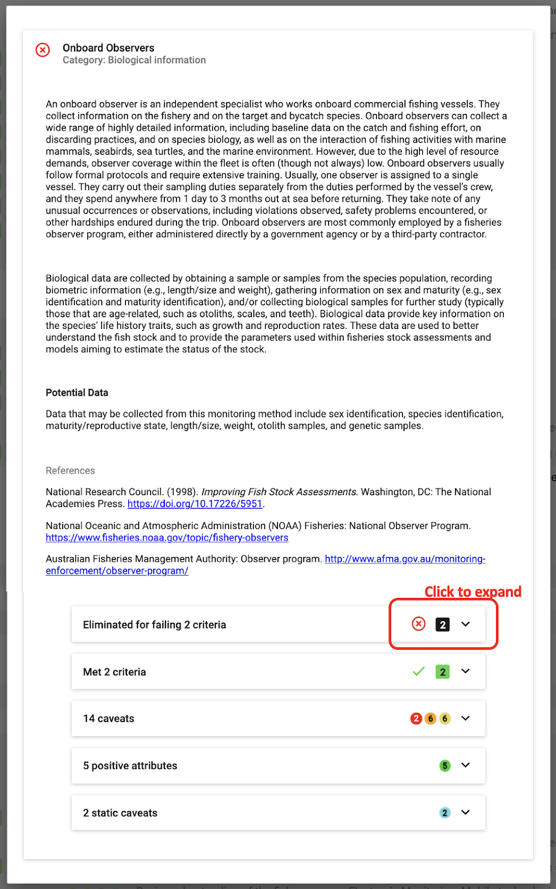
\includegraphics[width=0.5\linewidth]{images/option-description} 

}

\caption{Example of pop-up box that appears when clicking on each option. The user may click to expand each drop down menu for detail on each criteria or caveat (red label “Click to expand”).}\label{fig:opt-desc}
\end{figure}

\textbf{Criteria drop-down box (Figures \ref{fig:crit-drop-down}-\ref{fig:assessment-crit-drop-down})}: Each criteria drop-down shows the relevant question with the user's response bolded.

For the assessment section, when the minimum criteria are met, traffic light colors are assigned to indicate their relative uncertainty and subsequently the relative caution that should be taken (Figure \ref{fig:assessment-crit-drop-down}).

\begin{figure}

{\centering 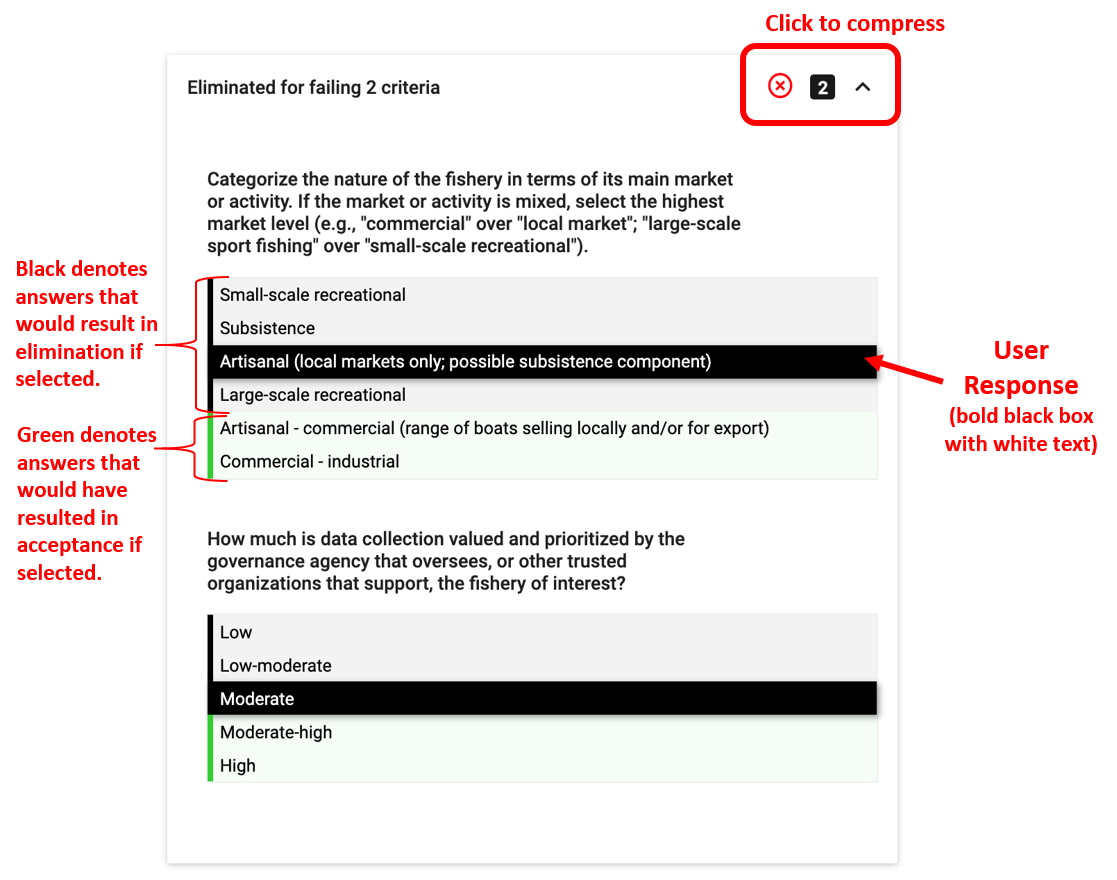
\includegraphics[width=0.75\linewidth]{images/crit-drop-down} 

}

\caption{Example drop-down menu with details for an option in the Data Collection section that was eliminated for failing two criteria. The bold, black box and white text indicates the user's answer to the question. The black answer options (black bar on left) indicate those that result in elimination if selected. The green answer options (green bar on left) indicate those that would have resulted in acceptance if selected.}\label{fig:crit-drop-down}
\end{figure}

\begin{figure}

{\centering 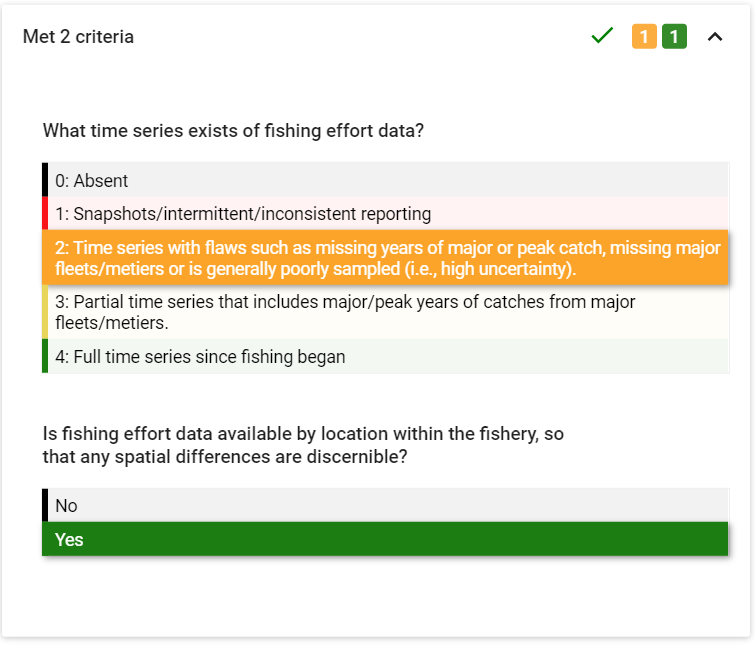
\includegraphics[width=0.75\linewidth]{images/assessment-crit-drop-down} 

}

\caption{Example drop-down menu with details for an option in the Assessment section that has passed criteria, but indicating the user to take caution regarding the uncertainty in removal data. Red indicates high uncertainty in the data. Green indicates low uncertainty. Bold box with white text indicates the user’s response.}\label{fig:assessment-crit-drop-down}
\end{figure}

\textbf{Caveat Drop-Down Box (Figures \ref{fig:cav-drop-down}-\ref{fig:static-cav-drop-down})}: Each individual caveat box displays the FishPath question with the user's answer in grey text, followed by caveat text related to the use of the option in the fishery in the context of that particular question response. The color of each box reflects the caveat color (see caveat descriptions above): cautionary caveats shaded yellow, orange or red; positive attributes shaded green; and static caveats shaded in light blue.

\begin{figure}

{\centering 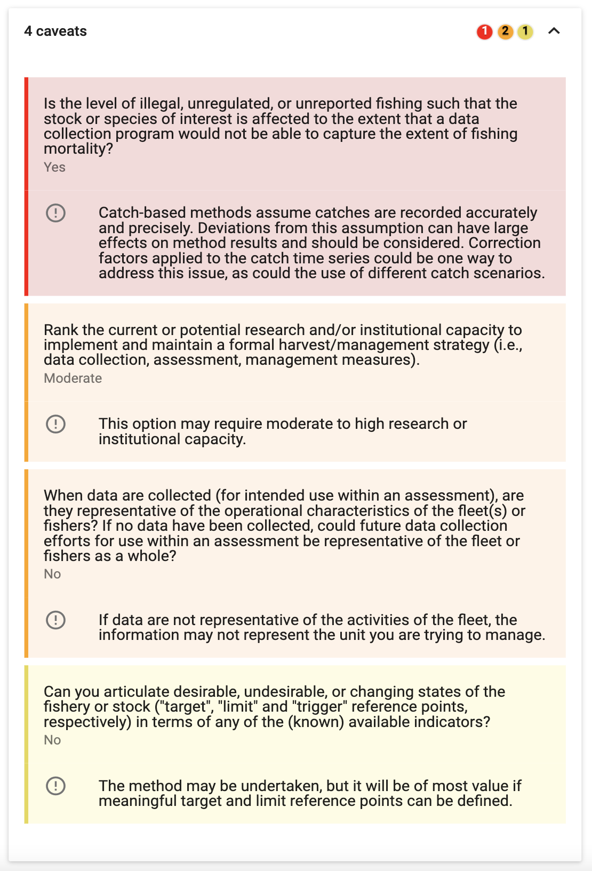
\includegraphics[width=0.75\linewidth]{images/cav-drop-down} 

}

\caption{Example caveat drop-down menu with details for an option for which questionnaire responses invoked 4 cautionary caveats (1 red, 2 orange, 1 yellow, as shown at the top right corner of the drop-down menu).}\label{fig:cav-drop-down}
\end{figure}

\begin{figure}

{\centering 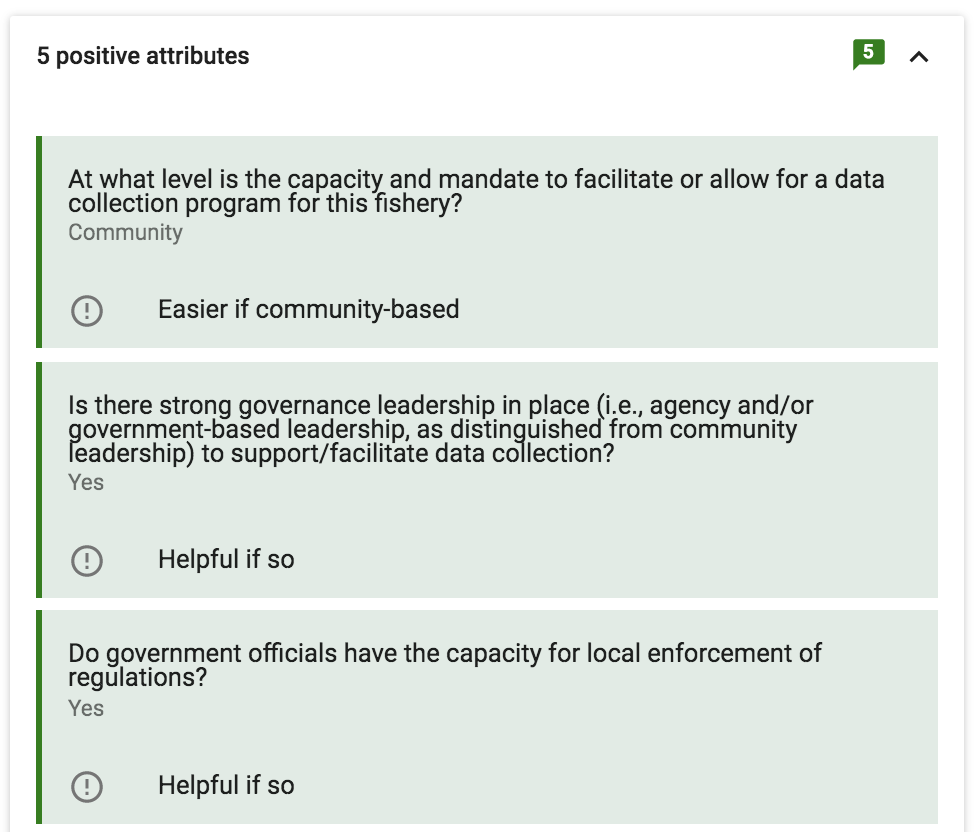
\includegraphics[width=0.75\linewidth]{images/pos-attr-drop-down} 

}

\caption{Example drop-down menu of positive attributes for an option for which questionnaire responses invoked 2 positive attributes (shown at the top right corner of the drop-down menu).}\label{fig:pos-attr-drop-down}
\end{figure}

\begin{figure}

{\centering 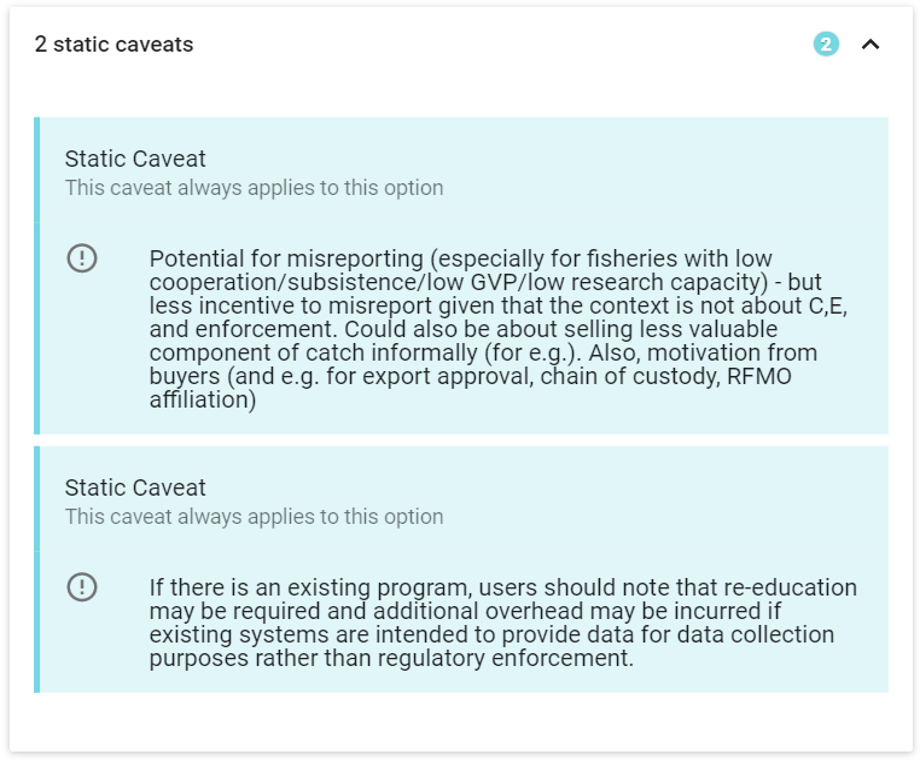
\includegraphics[width=0.75\linewidth]{images/static-cav-drop-down} 

}

\caption{Example static caveat drop-down menu for an option with 2 static caveats (shown at the top right corner of the drop-down menu). Each individual static caveat box displays grey text to note “This caveat always applies to this option”, and a short explanation of the static caveat.}\label{fig:static-cav-drop-down}
\end{figure}

\hypertarget{show-hidden-options-and-sort-options}{%
\section{Show Hidden Options and Sort Options}\label{show-hidden-options-and-sort-options}}

The ``Show Hidden Options'' Toggle (Figure \ref{fig:show-hidden-sort}) allows users to display or not display those options that have been ``hidden'' (greyed out) in the results table. When shown, ``hidden'' options will appear in grey.

\begin{figure}

{\centering 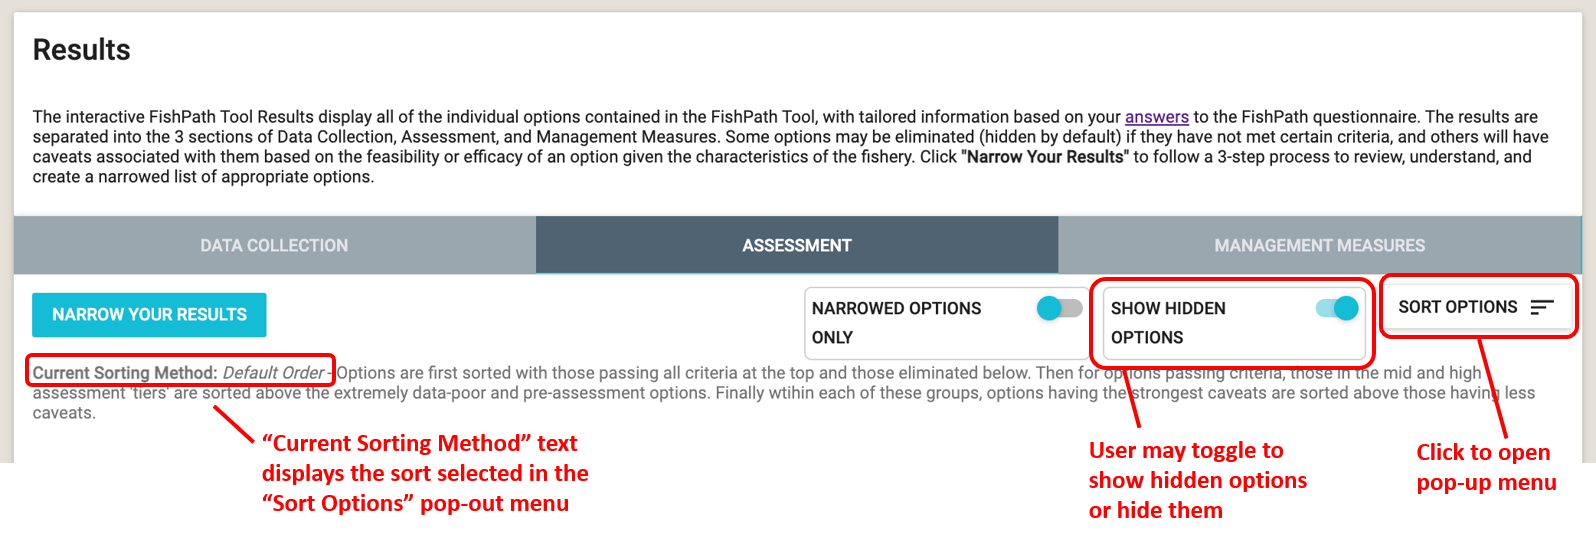
\includegraphics[width=0.75\linewidth]{images/show-hidden-options-and-sort} 

}

\caption{Results page with the “Show Hidden Options” Toggle and “Sort Options” in a red circle.}\label{fig:show-hidden-sort}
\end{figure}

The ``Sort Options'' functionality allows the user to arrange and view the options in different ways. This does not affect the results or shortlisting of options; it is merely a means to organize and display the results. The current sort selected is shown at the top of the results table at ``Current Sorting Method'' (Figure \ref{fig:show-hidden-sort}).

After clicking ``Sort Options'', a pop-up box (Figure \ref{fig:filter-and-sorting}) appears with the ability to sort the options by:

\begin{itemize}
\tightlist
\item
  In the Assessment section only, there is an additional option to select which category to display: ``Assessment Category'' or ``Assessment Output''.
\item
  \textbf{Default Order:} The default sort is to list all options that did not meet minimum criteria at the bottom (automatically greyed out as hidden options), with the options for which the highest number of cautionary caveats were invoked at the top for review.
\item
  \textbf{Customized Sort Order:} This allows users to ``drag and drop'' options into their preferred order.
\item
  \textbf{Sort by assessment `tiers' (Assessment Only):} Sorts options by assessment tier.
\item
  \textbf{Sort by option name:} Sorts options alphabetically by option name.
\item
  \textbf{Sort by category:} Sorts options alphabetically by category name. For the Assessment section, users first select the Category Display that they want to display and sort by.
\end{itemize}

Clicking a Sort option automatically sorts the options on the screen. After making selections on the Sort window, users can click outside of the pop-up onto the results table to return to the results.

\begin{figure}

{\centering 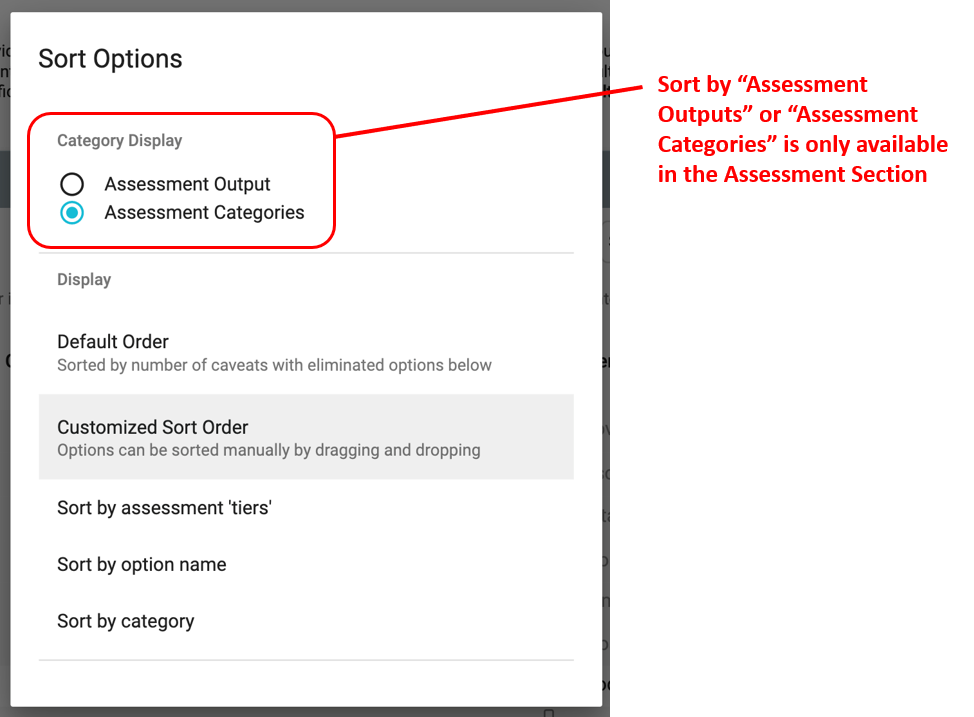
\includegraphics[width=0.5\linewidth]{images/filter-and-sorting-assessment} 

}

\caption{Sort Options pop-up box. The functionality to sort by “Assessment Outputs” or “Assessment Categories” is only available in the Assessment Section.}\label{fig:filter-and-sorting}
\end{figure}

\hypertarget{bookmarked-questions-and-influential-answers}{%
\section{Bookmarked Questions and Influential Answers}\label{bookmarked-questions-and-influential-answers}}

If the user scrolls to the bottom of the results screen (below results table), they are provided with a summary list of the questions bookmarked by the user, together with a list of ``Influential Answers'', and a ``See All Answers'' link.

\hypertarget{bookmarked-questions}{%
\subsection{Bookmarked Questions}\label{bookmarked-questions}}

All questions that were ``bookmarked'' during the questionnaire will be listed here (Figure \ref{fig:flagged-questions}). Users can select each question to get a detailed list of all caveats invoked or criteria not met based on the response. Users can select each question to change the answer, add notes, or remove the bookmark. It is highly recommended to review these questions so that users can change the answer or provide more detailed notes on the response, based on seeing how the response impacts results.

\begin{figure}

{\centering 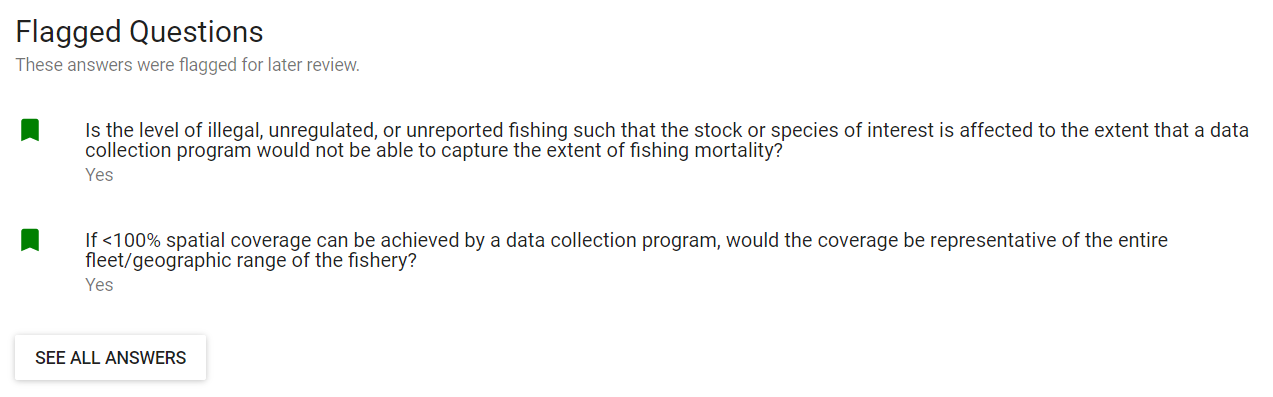
\includegraphics[width=0.95\linewidth]{images/flagged-questions} 

}

\caption{List of bookmarked questions.}\label{fig:flagged-questions}
\end{figure}

\hypertarget{influential-answers}{%
\subsection{Influential Answers}\label{influential-answers}}

The Influential Answers list is a summary of the questions and user responses that invoked the most eliminating criteria and greatest number of strong caveats (Figure \ref{fig:influential-answers}). The criteria and caveats invoked by these questions are displayed with icons to the left of the question by number and color strength.

It is recommended to review this list prior to entering the results narrowing process (described below), to better understand some of the key challenges facing the fishery. Users can select any question on this list to change the answer, add notes to the question, and see a list of all impacted options and their associated caveats (Figure \ref{fig:influential-answers-expanded}).

\begin{figure}

{\centering 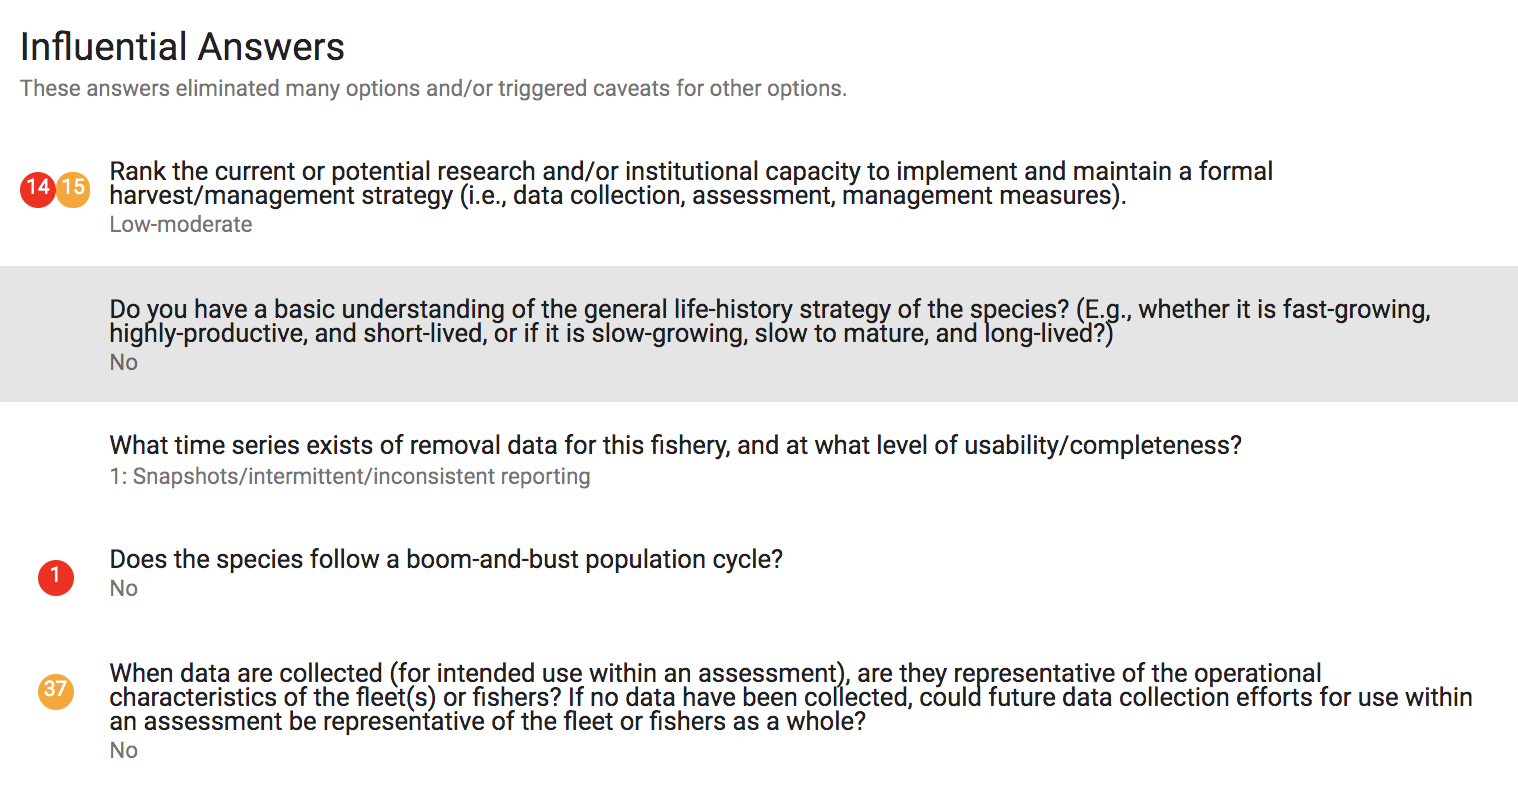
\includegraphics[width=0.95\linewidth]{images/influential-answers} 

}

\caption{List of influential answers.}\label{fig:influential-answers}
\end{figure}

\begin{figure}

{\centering 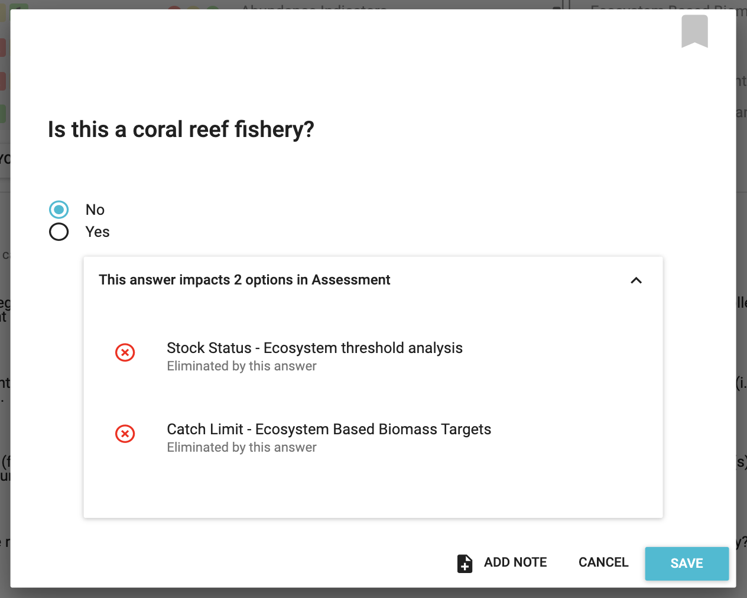
\includegraphics[width=0.75\linewidth]{images/influential-answers-expanded} 

}

\caption{When clicking on a question in the influential answer list, a pop-up is displayed, allowing the user to view impacted options.}\label{fig:influential-answers-expanded}
\end{figure}

\hypertarget{see-all-answers}{%
\subsection{See All Answers}\label{see-all-answers}}

There are 2 ways for the user to view all their answers to the questionnaire from the results page. First, at the top of the page, users can click the hyperlink ``answers'' in the paragraph under the ``Results'' header. Second, at the bottom of the page, there is a button labeled ``See All Answers''. After clicking either of these, the user is directed to the answers page. The answers page includes a full list of answers from all sections with corresponding details. This is a good resource for users wanting to review the questionnaire responses and associated notes for a fishery. Answers may also be changed and notes added, which update after clicking ``Save''.

\begin{figure}

{\centering 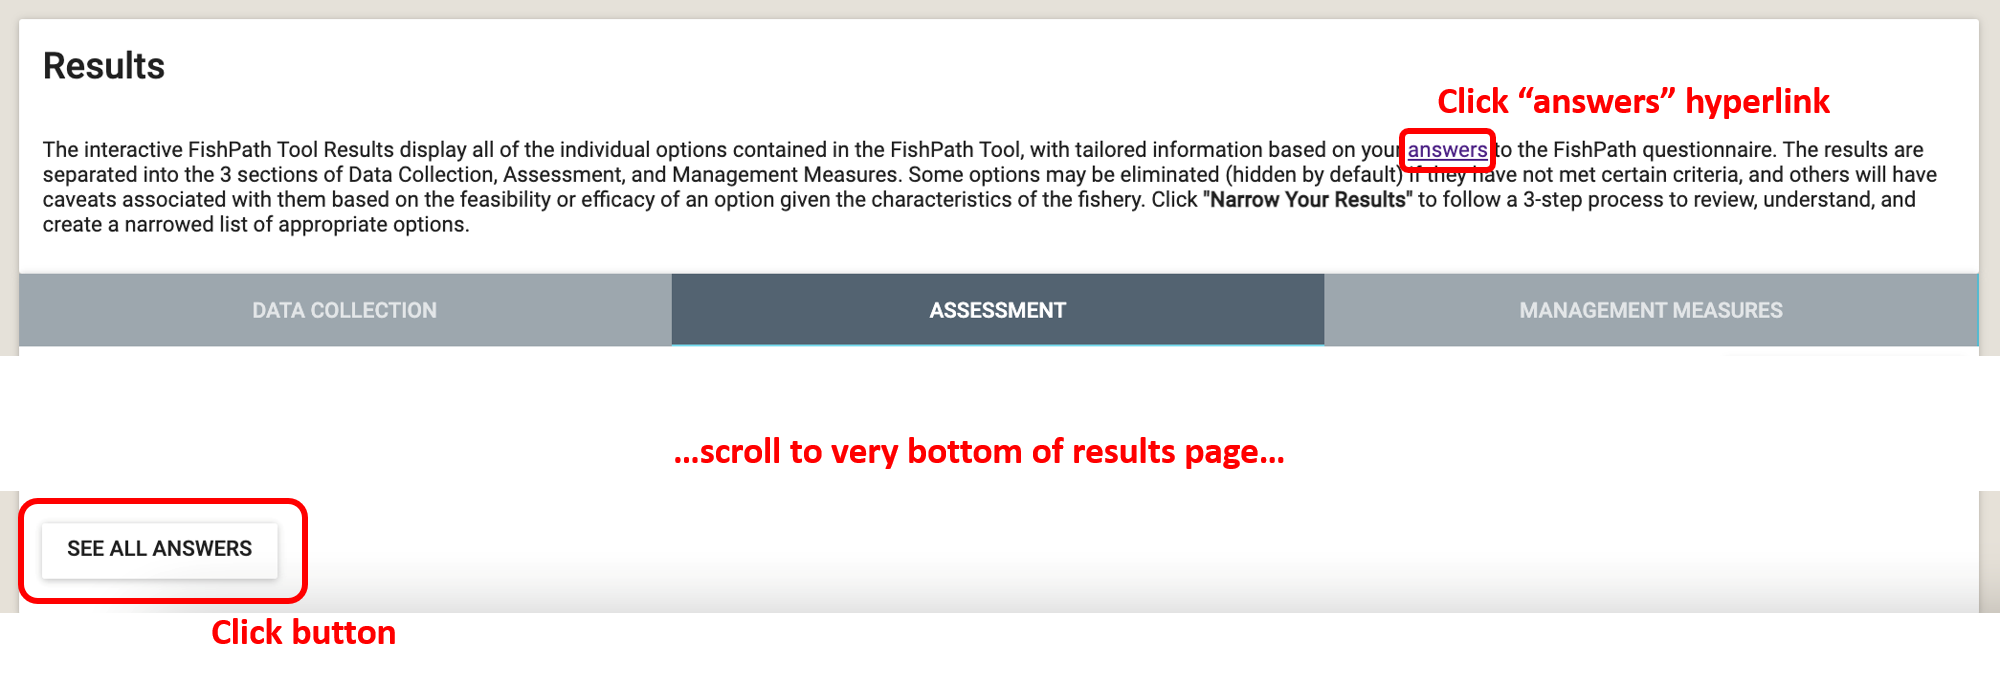
\includegraphics[width=0.75\linewidth]{images/see-all-answers-buttons} 

}

\caption{Two ways for users to view all answers to the questionnaire (red boxes) on the results page.}\label{fig:answers-buttons}
\end{figure}

\hypertarget{Results-Narrowing}{%
\section{Results Narrowing Process}\label{Results-Narrowing}}

The FishPath questionnaire process results in a long list of potential options that are presented to the user. The challenge is to then narrow this to a workable shortlist of options that can be reviewed in further detail, and around which a draft harvest strategy can be developed. This can be a daunting task, given the number of options, and the large amount of detail around the criteria and caveats.

As such, the Results Narrowing process prompts the user through a series of steps to review and narrow the options for their fishery, and to consider detail about the application of each option in the fishery. \textbf{The goal is to finish with a short list of defensible, appropriate, and documented options for the fishery.}

First, the user accesses the Results Narrowing process by selecting the ``Narrow Your Results'' button located above the Results Table in the Results Screen (See Figure \ref{fig:results-overview}).

After clicking on ``Narrow Your Results'', the user is directed to a step-wise results review process (Figure \ref{fig:results-review-header}). Each step of the results review process contains an ``Instructions'' box above the results with clear steps, as well as the ability to access different steps of the results review process through ``Back'', ``Exit Review'' and ``Next Step'' (Figure \ref{fig:results-review-header}). The blue ribbon across the top of the page shows which step of the process the user is at.

\begin{figure}

{\centering 
\includegraphics[width=0.95\linewidth]{images/results-review-header} 

}

\caption{Header for the results narrowing process.}\label{fig:results-review-header}
\end{figure}

The narrowing process (done as a group exercise or by independent users), consists of the following major steps:

\begin{enumerate}
\def\labelenumi{\arabic{enumi}.}
\tightlist
\item
  \textbf{Option Retention (Figure \ref{fig:review-step-1}):} The goal of the first step is to hide all options that are clearly not viable for the fishery due to failure to meet minimum criteria, logistical, political, or other major reasons. Users should review the list to hide these options, as well as un-hide options that they want to reinstate. Specific instructions are included on the screen in this step of the process, including questions to consider as narrowing the list. When complete, the user clicks on ``next step'' and a blue check will appear next to ``Option Retention'' in the blue ribbon at the top.
\end{enumerate}

\begin{figure}

{\centering 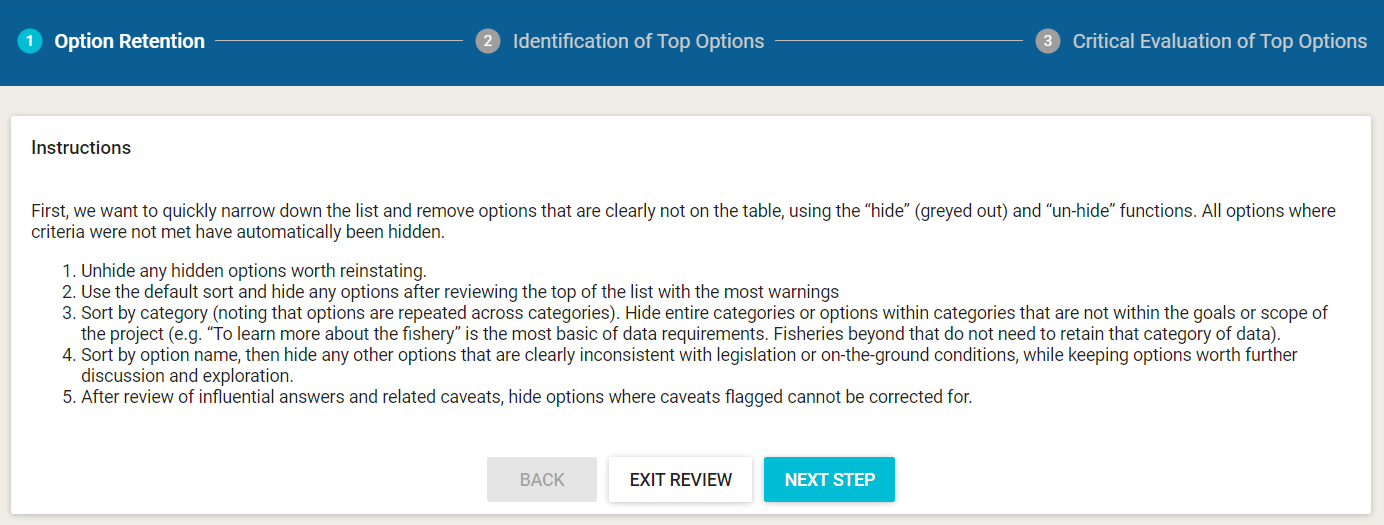
\includegraphics[width=0.95\linewidth]{images/review-step-1} 

}

\caption{Step 1, Option Retention, in the results review process.}\label{fig:review-step-1}
\end{figure}

\begin{enumerate}
\def\labelenumi{\arabic{enumi}.}
\setcounter{enumi}{1}
\tightlist
\item
  \textbf{Identification of Top Options (Figure \ref{fig:review-step-2}):} In this step, users review each remaining option to identify a short list of starred options that will be seriously considered and explored in more detail. Users should familiarize themselves with the sorting feature and the influential answer list (see above) to facilitate this process. When comparing options, users should compare the criteria, cautionary caveats, and positive attributes. Specific instructions are included on the screen in this step of the process. As the user ``stars'' options, a black number circled in orange appears next to the step in the blue ribbon at the top of the page. The number represents the number of top options that have been starred. A blue check mark will appear in the blue ribbon for this step once the user clicks the ``next step'' button.
\end{enumerate}

\begin{figure}

{\centering 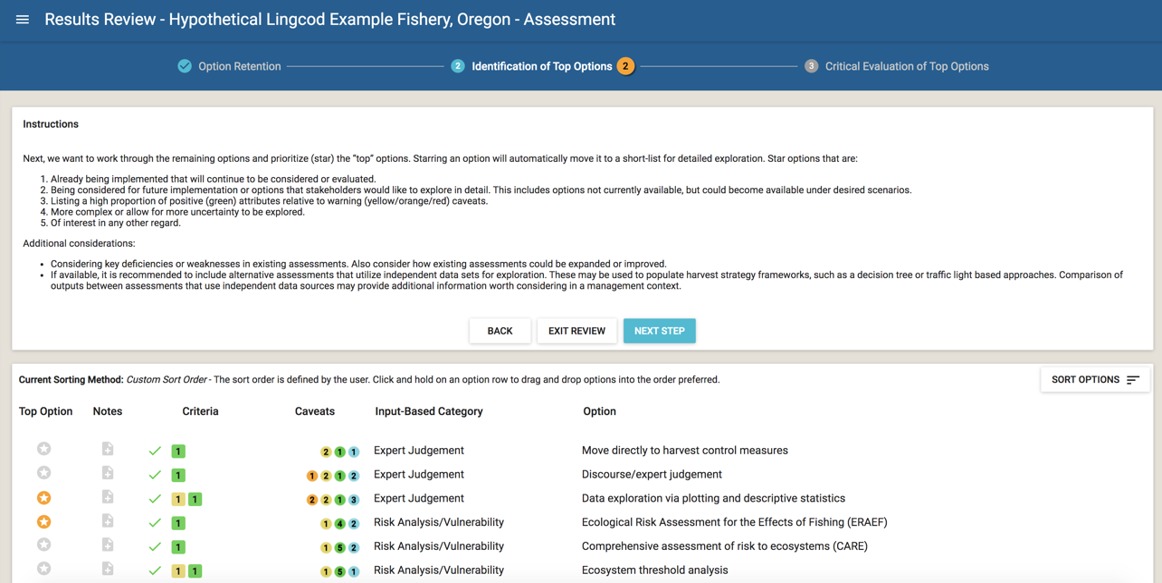
\includegraphics[width=0.95\linewidth]{images/review-step-2} 

}

\caption{Step 2, Identification of Top Options, in the results review process.}\label{fig:review-step-2}
\end{figure}

\begin{enumerate}
\def\labelenumi{\arabic{enumi}.}
\setcounter{enumi}{2}
\tightlist
\item
  \textbf{Critical Evaluation of Top Options (Figure \ref{fig:review-step-3}):} In the final step, users can more critically evaluate the top options by considering each criterion and caveat in complete detail, and, potentially, ranking the options in order of potential.
\end{enumerate}

\begin{figure}

{\centering 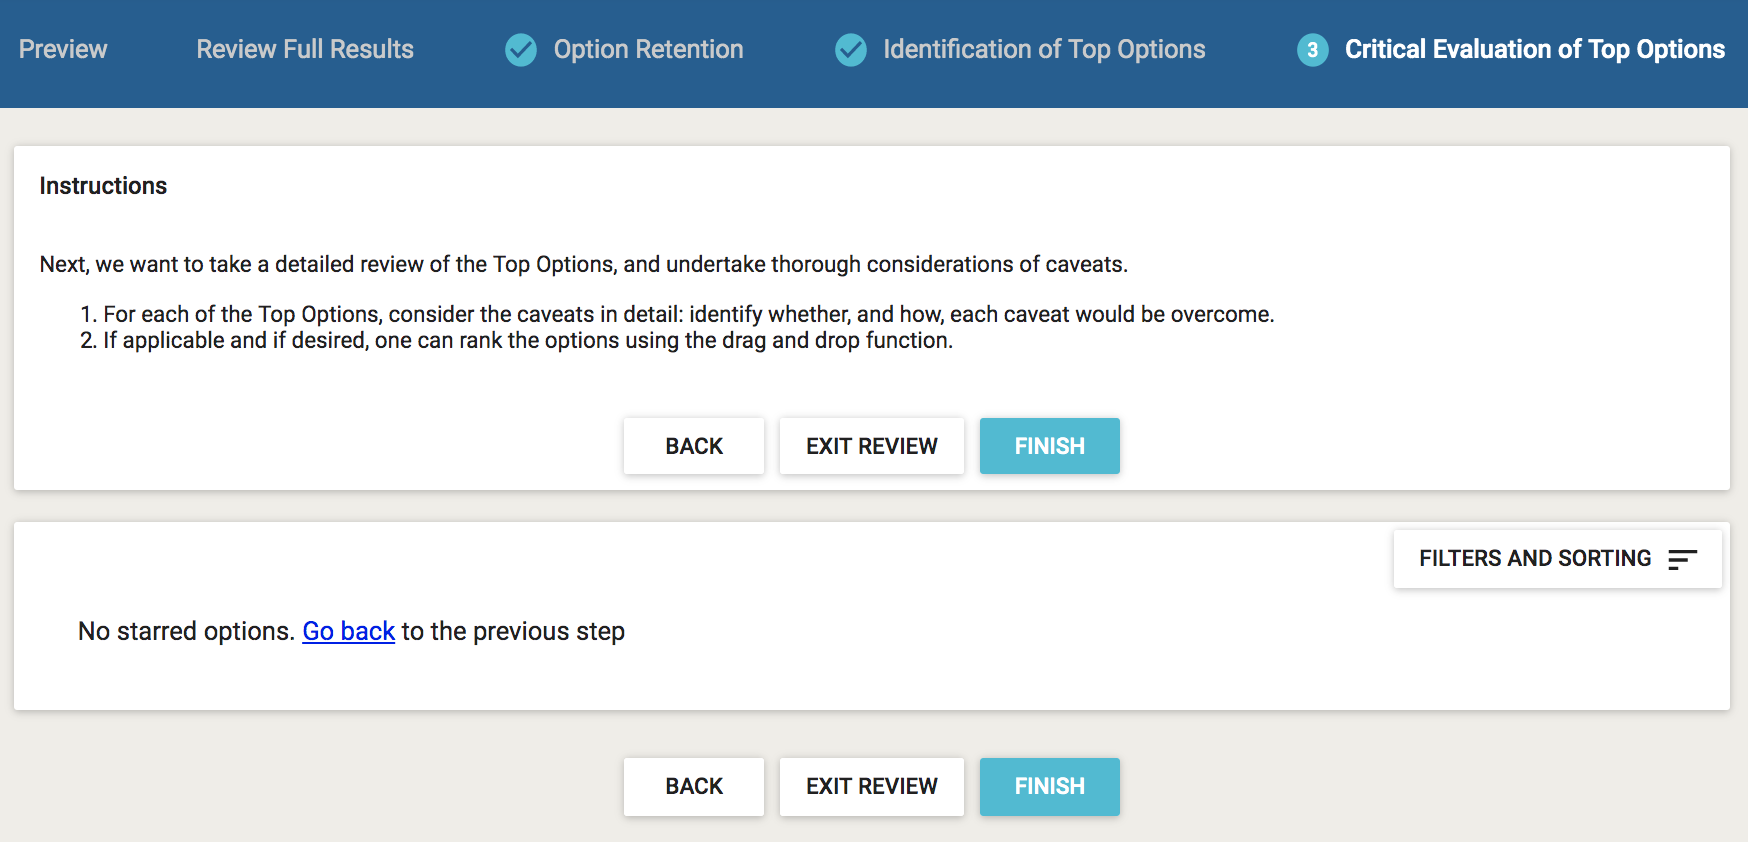
\includegraphics[width=0.95\linewidth]{images/review-step-3} 

}

\caption{Step 3, Critical Evaluation of Top Options, in the results review process.}\label{fig:review-step-3}
\end{figure}

Upon fishing this step, users should click ``Finish'' to finalize results and return to the results page. The results will then be filtered to only show Narrowed Options. Users may still toggle between the Narrowed Options and all options. A PDF report of the Narrowed Options can be generated by clicking the ``Generate PDF Report'' button, while using the filter to show Narrowed options only.

\hypertarget{Results-Actions}{%
\section{Actions to Share Results and Edit Fishery Info}\label{Results-Actions}}

At the top of the Results Page, the user may either ``Share'', ``Export CSV'', ``Generate PDF Report'', ``Copy'', or ``Edit Name and Details'' for their fishery (Figure \ref{fig:results-components}).

\begin{itemize}
\tightlist
\item
  \textbf{Share:} This will generate a link that allows the user to share fishery results with others. The user simply needs to send the link and the recipient will have \protect\hyperlink{view-only-mode-shared-fishery}{\textbf{view-only access}} to this fishery from their active account. A shared fishery can be saved under someone else's FishPath account, and they can make a copy of it to separately edit, if needed. Tip: when creating a copy of a shared fishery in a user account, it is useful to rename the fishery so that edits are tracked under this new name.
\item
  \textbf{Export CSV:} This allows users to export the question and answer list from the saved questionnaire, as well as a simple results file, as a .csv file.
\item
  \textbf{Generate PDF Report:} Allows the user to create a .PDF of the FishPath results, with all notes captured. The PDF report provides detailed information on each option and their associated caveats and criteria related to the fishery. Users can select to see a report for the ``full list'' of options, or for a specified list of ``top options''.
\item
  \textbf{Copy Fishery:} This allows users to make a copy of a fishery's results, either their own or from a shared link. The user may update the fishery information for the new copied fishery before confirming the copy. The copy will be saved in the user's Dashboard.
\item
  \textbf{Edit Name and Details:} This allows users to edit the information entered on the Fishery Information form (name, species, geography, etc.).
\end{itemize}

\hypertarget{view-only-mode-shared-fishery}{%
\section{View-Only Mode (Shared Fishery)}\label{view-only-mode-shared-fishery}}

Users may \protect\hyperlink{Results-Actions}{\textbf{share a FishPath questionnaire and results}} with other audiences as a shared link, but the answers and results cannot be edited by other users. This allows the results to be maintained.

When clicking the shared link, the user will view results in a ``View-Only'' mode (Figure 32). In this mode, the user will be able to explore the results and answers provided by the original user; however, the user will not be able to make any changes. The user can sort and filter options, yet editing functionality is disabled, such as the ability to update questionnaire answers or add notes. Greyed out options indicate options hidden by the original user. If notes taken by the original user exist, they will appear with a yellow note icon in view-only mode.

The user may ``Copy Fishery'', allowing them to edit fishery details such as name and location, and then make any edits. This ``copied fishery'' will appear on their Dashboard.

\begin{figure}

{\centering 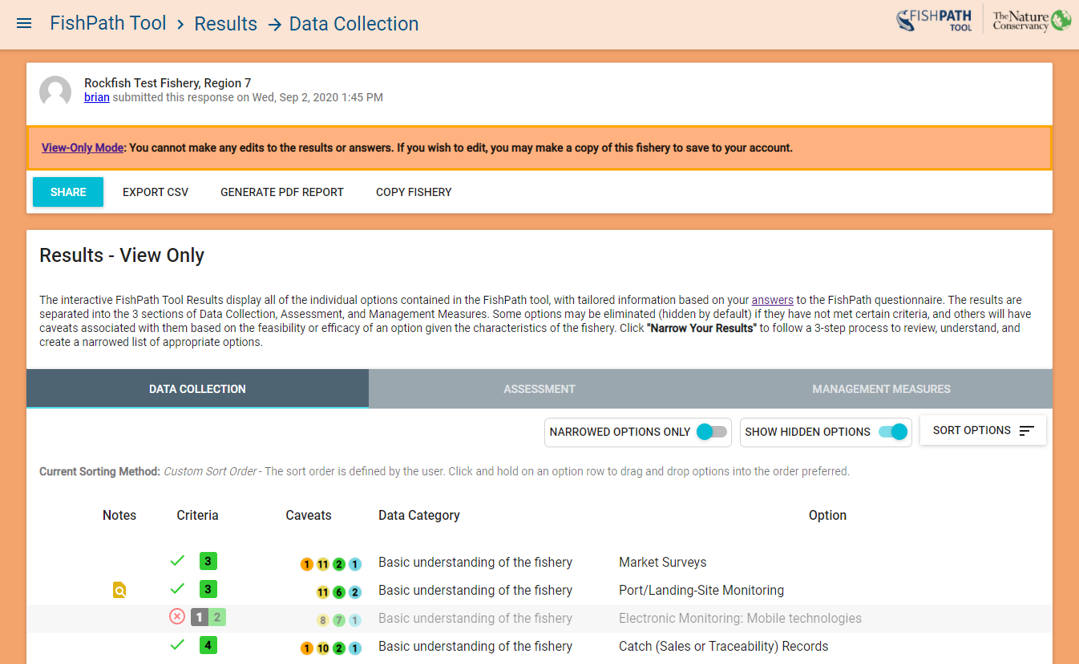
\includegraphics[width=0.95\linewidth]{images/view-only} 

}

\caption{The “View-Only” mode of FishPath Tool results.}\label{fig:view-only}
\end{figure}

\hypertarget{appendix-appendix}{%
\appendix}


\hypertarget{fishpath-tool-frequently-asked-questions-faqs}{%
\chapter{FishPath Tool Frequently Asked Questions (FAQs)}\label{fishpath-tool-frequently-asked-questions-faqs}}

\hypertarget{faq-feedback}{%
\paragraph{How do I submit feedback about content or user experience?}\label{faq-feedback}}

FishPath benefits from the expertise and feedback of the global community of FishPath tool users. Users are encouraged to submit feedback about the FishPath tool, ultimately helping to improve the tool. There are two ways to submit feedback:

\begin{enumerate}
\def\labelenumi{\arabic{enumi}.}
\tightlist
\item
  The ``Submit Feedback'' button on FishPath Tool Dashboard. The user is prompted to categorize their feedback as ``Content Related'' or ``Software Issue''.
\item
  Email \href{mailto:support@fishpath.org}{\nolinkurl{support@fishpath.org}}
\end{enumerate}

\hypertarget{faq-content-updates}{%
\paragraph{How does the FishPath Tool content (questions, options, caveats, etc.) get updated? And how often?}\label{faq-content-updates}}

The FishPath team is composed of practicing fisheries managers and scientists who stay up to date on the changing field of fisheries research. The Tool is maintained with the aim of being as current with fishery management practices, science and literature as possible. We also strive to correct any mistakes found in the Tool as quickly as possible. In order to do this, content updates can be made at any time.

Suggestions from users regarding the content is also greatly appreciated and encouraged. We recognize that fisheries occur in a wide variety of contexts and our small team cannot know every possible scenario and caveat. Any feedback will get a full review and be incorporated into the Tool as needed.

Every time a user logs in, the Tool will use the most up to date version of the Tool content. No action is needed to receive the updates, even if the questionnaire is already completed. If a new question has been added after a user has completed the questionnaire, a prompt will appear to answer that question before returning to the results screen.

\hypertarget{faq-stay-updated}{%
\paragraph{How do I stay updated on changes to the FishPath Tool questionnaire or content?}\label{faq-stay-updated}}

A brief summary of any major changes is documented in the biannual newsletter. A changelog is under development which will document all the changes made after April 2021.

\hypertarget{faq-copy-fisheries}{%
\paragraph{Are answers to new questions also updated in ``copied fisheries''?}\label{faq-copy-fisheries}}

Once a fishery is copied, changes in the original or copied fishery will have no effect on the other.

\hypertarget{faq-internet}{%
\paragraph{Does the FishPath Tool need the internet to run?}\label{faq-internet}}

The FishPath Tool does require an internet connection to load and function properly. However, the Tool has been designed to handle poor or intermittent internet connections. Once logged in, the Tool can partially function without the internet. If the internet cuts out or lags while working, the Tool will store any answers to questions or changes made while offline in the browser until it is able to reconnect with the server and save the changes. The \protect\hyperlink{saving-status-toolbar}{saving status toolbar} across the bottom of the screen lets the user know if any changes have not been able to be saved to the server. Closing the window or navigating away from the Tool when there are unsaved changes, will cause those changes to be lost.

\hypertarget{faq-question-numbering}{%
\paragraph{Why does the number of questions for each section appear to change?}\label{faq-question-numbering}}

Many of the questions in the questionnaire are relevant to multiple sections. Once you answer a question that affects multiple sections, the Tool will not repeat that question again when completing the questionnaire for another section. For example, before starting the questionnaire for any section, there are 41 questions in Data Collection, 50 questions in Assessment, and 44 in Management Measures. A user starts by completing the Data Collection questionnaire. 6 of those questions also apply to Assessment and 14 apply to Management Measures as well. If the user answers the Assessment section next, instead of being asked all 50 questions, only 44 would be asked, since 6 of the questions have already been answered when completing the Data Collection questionnaire. Likewise, if the user answers the Management Measures section next, only 30 questions would be asked.

\hypertarget{terms}{%
\chapter{FishPath Tool Terms of Service}\label{terms}}

\textbf{Last revised on October 23, 2018}

The Nature Conservancy (``TNC,'' ``we,'' ``us,'' or ``our'') are pleased to provide FishPath and related software, data, websites, instructions, and services (``FishPath'') to you. If you are using FishPath on behalf of a business (such as your employer), that business accepts these terms of service (``Terms'') by your use. In that case, the words ``You'' and ``Your'' in these Terms refer to both you and that business.

The Terms govern Your access to and use of FishPath, so please carefully read them and Our Privacy Policy before using FishPath. By registering on the FishPath websites and using FishPath, You agree to be bound by these Terms and by our Privacy Policy. If You don't agree with these Terms and our Privacy Policy, You cannot use FishPath or FishPath data in any way or at any time.

\hypertarget{fishpath-data-your-rights-and-your-privacy}{%
\subsubsection*{FishPath Data: Your Rights and Your Privacy}\label{fishpath-data-your-rights-and-your-privacy}}
\addcontentsline{toc}{subsubsection}{FishPath Data: Your Rights and Your Privacy}

We developed FishPath as a user-friendly application to help users diagnose the challenges in their fishery and select appropriate options for data collection, stock assessment, and management measures. FishPath allows You to use Your fishery information (Your ``Submission''). Your Submission to FishPath is voluntary. If You submit information to FishPath, these Terms do grant us the right to see and use Your Submission to improve the functionality of the tool as appropriate. We may copy and share an anonymized aggregation of information from submissions, potentially including Your Submission, with the public. However, we will not share Your submission nor Your information in any non aggregated format.

Please refer to our \href{https://www.nature.org/en-us/about-us/who-we-are/accountability/privacy-policy/}{Privacy Policy} for a description of how we collect, use and disclose FishPath information, including Your Submission. We have the right to withdraw or change FishPath. As we describe below, we will not be liable to You if for any reason all or any part of FishPath is unavailable at any time or for any length of time.

\hypertarget{your-responsibilities}{%
\subsubsection*{Your Responsibilities}\label{your-responsibilities}}
\addcontentsline{toc}{subsubsection}{Your Responsibilities}

Only make a Submission if You have all necessary rights to share the information with us, including but not limited to use with FishPath. You are solely responsible for your conduct and Your Submission while using FishPath. It is Your responsibility to ensure that You have the rights or permission needed to comply with these Terms.

Respect the law. Do not use FishPath for any fraudulent or unlawful purpose including violations of statutory, regulatory or contractual law. Respect copyright, privacy, trade secret, data protection, fish \& wildlife and all other laws. Do not attempt to impersonate any other individual on FishPath; if You identify yourself, You must always use Your true identity.

Without our express written consent, You may not use, display, mirror, or frame FishPath, any element within FishPath, or any proprietary elements belonging to us (including but not limited to our logos and marks). In addition to adhering to all applicable laws and regulations, You may NOT do any of the following:

\begin{itemize}
\tightlist
\item
  resell FishPath or data from FishPath, or any portion thereof;
\item
  access or search the FishPath data by using any engine, software, tool, agent, device or mechanism (including spiders, robots, crawlers, data mining tools or the like) other than the software and/or search agents that We provide or authorize;
\item
  probe, scan, tamper with, or test the vulnerability of FishPath or any of our systems or networks;
\item
  avoid, breach, deactivate, impair, or circumvent any security or authentication measures, including those that protect FishPath and its data;
\item
  attempt to decipher, decompile, disassemble or reverse engineer any of the software used to provide FishPath;
\item
  interfere with, or attempt to interfere with, the access of any user, host or network, including, without limitation, by sending a virus, overloading, or flooding FishPath;
\item
  encourage or enable anyone else to do any of the foregoing.
\end{itemize}

We have the right to investigate violations of these Terms or conduct that affect FishPath or our systems or networks. We may also consult and cooperate with law enforcement authorities to prosecute users who violate the law.

\hypertarget{rights-you-grant-in-your-information}{%
\subsubsection*{Rights You Grant in Your Information}\label{rights-you-grant-in-your-information}}
\addcontentsline{toc}{subsubsection}{Rights You Grant in Your Information}

By making Your Submission, You grant us a non-exclusive, transferable, sublicensable, worldwide, perpetual, royalty-free license to use, copy, modify, create derivative works based upon, distribute, publicly display, publicly perform and distribute Your Submission. We will not, however, share or distribute specific notes You submit for Your fishery.

\hypertarget{rights-that-we-grant-you}{%
\subsubsection*{Rights That We Grant You}\label{rights-that-we-grant-you}}
\addcontentsline{toc}{subsubsection}{Rights That We Grant You}

Subject to Your compliance with these Terms, we grant You a limited, non-exclusive, non-transferable, non-sublicensable, worldwide, royalty-free license to use the FishPath software, instructions, and websites and to view, copy, display, and create derivative works from the FishPath output that we make available from the FishPath site for Your management of Your fishery.

You may not: (i) copy, modify or create derivative works based on the FishPath software; (ii) distribute, transfer, sublicense, lease, or rent the FishPath software to any third party; or (iii) reverse engineer, decompile or disassemble the FishPath software.

Using FishPath or uploading Data does not give You ownership of any intellectual property rights in FishPath (other than your own Submission). We and our licensors exclusively own all right, title and interest in and to FishPath, including all associated intellectual property rights. You acknowledge that copyright, trademark, and other laws of the United States and foreign countries protect FishPath. You agree not to remove, alter or obscure any copyright, trademark, service mark or other proprietary rights notices incorporated in or accompanying FishPath.

These Terms do not grant You the right to use any of our branding or logos or names. You must not use our names or logos or branding without our written permission.

\hypertarget{modifying-our-terms-of-service}{%
\subsubsection*{Modifying our Terms of Service}\label{modifying-our-terms-of-service}}
\addcontentsline{toc}{subsubsection}{Modifying our Terms of Service}

We may update these Terms from time to time, in our sole discretion. We may notify You of such updates by any reasonable means, such as by posting the revised Terms on the FishPath website. Please look at the ``LAST UPDATED'' legend above to see when these Terms were last revised. Your use of FishPath after the posting of any revised Terms means that You accept and agree to be bound by the revised Terms. If You don't agree to be bound by the revised Terms, then You may not use FishPath anymore. You can stop using FishPath at any time. We may also stop providing FishPath or add or create new limits to FishPath at any time.

\hypertarget{disclaimers-limited-liability-and-indemnity}{%
\subsubsection*{Disclaimers, Limited Liability and Indemnity}\label{disclaimers-limited-liability-and-indemnity}}
\addcontentsline{toc}{subsubsection}{Disclaimers, Limited Liability and Indemnity}

As we describe in more detail below, FishPath and its data are a general information resource and are provided solely ``AS IS'' and ``AS AVAILABLE'' without warranty of any kind. You should not construe publication of FishPath data as a warranty or guarantee of the quality or availability of any goods or services or technical support.

\hypertarget{disclaimers-and-limitation-of-liability}{%
\subsubsection*{DISCLAIMERS AND LIMITATION OF LIABILITY}\label{disclaimers-and-limitation-of-liability}}
\addcontentsline{toc}{subsubsection}{DISCLAIMERS AND LIMITATION OF LIABILITY}

ALL CONTENT ON FISHPATH IS PROVIDED ``AS IS'' AND ``AS AVAILABLE'' WITHOUT WARRANTY OF ANY KIND, EITHER EXPRESS OR IMPLIED. WITHOUT LIMITING THE FOREGOING, WE EXPLICITLY DISCLAIM ANY AND ALL WARRANTIES OF MERCHANTABILITY, FITNESS FOR A PARTICULAR PURPOSE, QUIET ENJOYMENT, OR NON-INFRINGEMENT, AND ANY AND ALL WARRANTIES ARISING OUT OF COURSE OF DEALING OR USAGE OF TRADE. TNC MAKES NO WARRANTY AS TO THE QUALITY, ACCURACY, COMPLETENESS, TIMELINESS, OR RELIABILITY OF FISHPATH OR ANY FISHPATH CONTENT. YOUR USE OF FISHPATH IS AT YOUR SOLE RISK.

TNC MAKES NO REPRESENTATIONS OR WARRANTIES THAT YOUR USE OF FISHPATH WILL MEET YOUR NEEDS OR BE UNINTERRUPTED, SECURE, OR ERROR FREE. USERS ARE RESPONSIBLE FOR TAKING ALL NECESSARY PRECAUTIONS TO ENSURE THAT ANY CONTENT YOU MAY OBTAIN FROM THE SERVICES IS FREE OF VIRUSES OR OTHER HARMFUL CODE.

TO THE MAXIMUM EXTENT PERMITTED BY LAW, WE SHALL NOT BE LIABLE FOR CREATING, PRODUCING, MAINTAINING, OPERATING, OR PROVIDING FISHPATH OR FISHPATH CONTENT, UNDER ANY THEORY BASED IN CONTRACT, WARRANTY, TORT (INCLUDING NEGLIGENCE), PRODUCT LIABILITY, STRICT LIABILITY, OR OTHER LEGAL THEORY. THIS LIMITATION ON LIABILITY INCLUDES ANY AND ALL INDIRECT, INCIDENTAL, SPECIAL, EXEMPLARY OR CONSEQUENTIAL DAMAGES, INCLUDING LOST PROFITS, LOSS OF DATA OR GOODWILL, SERVICE INTERRUPTION, COMPUTER DAMAGE OR SYSTEM FAILURE OR THE COST OF SUBSTITUTE SERVICES ARISING OUT OF OR IN CONNECTION WITH THESE TERMS OR FROM THE USE OF OR INABILITY TO USE FISHPATH, EVEN IF WE HAVE BEEN ADVISED OF THE POSSIBILITY OF SUCH DAMAGES.

THE ABOVE EXCLUSIONS AND LIMITATIONS OF DAMAGES ARE FUNDAMENTAL ELEMENTS OF THE BASIS OF THE BARGAIN BETWEEN YOU AND US.

\hypertarget{indemnity}{%
\subsubsection*{Indemnity}\label{indemnity}}
\addcontentsline{toc}{subsubsection}{Indemnity}

You agree to release, indemnify, defend and hold harmless TNC, our subsidiaries and affiliates, and our and their respective officers, directors, agents, partners and employees, from and against any claims, disputes, demands, liabilities, damages, losses, and costs and expenses, including, without limitation, reasonable legal and accounting fees arising out of or in any way connected with (i) Your access to or use of FishPath, (ii) Your Submission, or (iii) Your violation of these Terms.

\hypertarget{termination}{%
\subsubsection*{Termination}\label{termination}}
\addcontentsline{toc}{subsubsection}{Termination}

We may terminate Your access to and use of FishPath, at our sole discretion, at any time and without notice to You. Upon any termination, discontinuation or cancellation of FishPath, all provisions of these Terms that by their nature should survive will survive. This includes, for example ownership provisions, warranty disclaimers, and limitations of liability.

\hypertarget{general-terms}{%
\subsubsection*{General Terms}\label{general-terms}}
\addcontentsline{toc}{subsubsection}{General Terms}

These Terms are the entire and exclusive agreement between You and us regarding FishPath, and they supersede any prior agreements between You and us regarding FishPath.

These terms do not create any third party beneficiary rights. You may not assign or transfer these Terms, by operation of law or otherwise, without our prior written consent. Subject to the foregoing, these Terms will bind your successors and permitted assigns. We may freely assign or transfer these Terms without restriction.

If You do not comply with these Terms, and we do not take action right away, this does not mean that we are giving up any rights that we may have to take action in the future or seek all available remedies.

If it turns out that a particular provision of these Terms is not fully valid or enforceable, that provision will be enforced to the maximum extent permissible, and this will not affect any other Terms.

All claims arising out of this Agreement or relating to FishPath will be governed by the laws of the State of California, excluding the application of its conflicts of law rules. Any legal action or proceeding arising out of this Agreement or relating to these Services shall be brought exclusively in a state or federal court in or for San Francisco, California. You agree that any and all disputes, claims and causes of action arising out of, or connected with these Terms or Your Submission shall be resolved individually, without resort to any form of class action.

\hypertarget{glossary}{%
\chapter{Glossary}\label{glossary}}





Note: The \href{http://www.fao.org/fishery/glossary/en}{FAO Term Portal - Fisheries} has some of the definitions in multiple languages.

\hypertarget{absolute-abundance}{%
\subsection{Absolute Abundance}\label{absolute-abundance}}

The total number of a kind of fish in a population; this is rarely known, and usually estimated from the relative abundance.

Source: \href{https://repository.library.noaa.gov/view/noaa/12856}{Blackhart, K., Stanton, D. G., \& Shimada, A. M. (2006). \emph{NOAA fisheries glossary.} United States Department of Commerce, National Oceanic and Atmospheric Administration.}

\hypertarget{b0-virgin-biomass}{%
\subsection{B0 (Virgin Biomass)}\label{b0-virgin-biomass}}

``B0'', or virgin biomass, refers to the average biomass of a stock that has yet not been fished. It is generally calculated as the long-term average biomass value expected in the absence of fishing mortality. In production models, B0 is also known as carrying capacity. It is often used as a reference value to assist the relative health of a stock, monitoring changes in the ratio between current and virgin biomass (B/B0).

Source: Restrepo V. (1999): Annotated Glossary of Terms in Executive Summary Reports of the International Commission for the Conservation of Atlantic Tunas' Standing Committee on Research and Statistics (SCRS), \emph{ICCAT}.

via \href{http://www.fao.org/fishery/glossary/en}{FAO Term Portal - Fisheries}

\hypertarget{bias}{%
\subsection{Bias}\label{bias}}

An effect which deprives a statistical result of representativeness by systematically distorting it, as distinct from a random error which may distort on any one occasion but balances out on the average.

Source: \href{https://stats.oecd.org/glossary/detail.asp?ID=3605}{OECD Glossary}

\hypertarget{biological-overfishing}{%
\subsection{Biological Overfishing}\label{biological-overfishing}}

Catching such a high proportion of one or all age classes in a fishery as to reduce yields and drive stock biomass, and spawning potential below safe levels. Can involve both growth overfishing and recruitment overfishing. With reference to a surplus production model, biological overfishing occurs when fishing levels are higher that those required for extracting the maximum sustainable yield (MSY) of a resource.

Source: Garcia, S.M. (Comp.). 2009. Glossary. In Cochrane, K. and S.M. Garcia. (Eds). \emph{A fishery manager's guidebook}. FAO and Wiley-Blackwell:473-505.

via \href{http://www.fao.org/fishery/glossary/en}{FAO Term Portal - Fisheries}

\hypertarget{boom-and-bust-population-cycle}{%
\subsection{Boom and Bust Population Cycle}\label{boom-and-bust-population-cycle}}

Species that follow boom-and-bust cycles display high volatility in their population dynamics. This means that their availability is sudden, extreme, and unpredictable.

Source: FishPath Team

\hypertarget{bycatch}{%
\subsection{Bycatch}\label{bycatch}}

Part of a catch of a fishing unit taken incidentally in addition to the target species towards which fishing effort is directed. Some or all of it may be returned to the sea as discards, usually dead or dying

Source: Modified from FAO (1998): Guidelines for the routine collection of capture fishery data

via \href{http://www.fao.org/fishery/glossary/en}{FAO Term Portal - Fisheries}

\hypertarget{capital-stuffing}{%
\subsection{Capital Stuffing}\label{capital-stuffing}}

Costly investments in vessel or gear improvements, to outcompete others for a larger share of available fish. This often leads to higher levels of catch than those intended by managers.

Source: Townsend, R. E. (1985). On capital-stuffing in regulated fisheries. \emph{Land
Economics, 61}(2), 195. \url{https://doi.org/10.2307/3145812}

via Anderson CM, Krigbaum MJ,
Arostegui MC, et al.~How commercial fishing effort is managed. \emph{Fish Fish}. 2018;00:1--18. \url{https://doi.org/10.1111/faf.12339}

\hypertarget{carrying-capacity-k}{%
\subsection{Carrying Capacity (K)}\label{carrying-capacity-k}}

The maximum population of a species that a specific ecosystem can support indefinitely without deterioration of the character and quality of the resource. It represents the point of balance between reproduction potential and environmental constraints.

Source: Scialabba N. (ed.), 1998. \emph{Integrated Coastal Area Management and Agriculture, Forestry and Fisheries}. FAO Guidelines, 256p.

via \href{http://www.fao.org/fishery/glossary/en}{FAO Term Portal - Fisheries}

\hypertarget{catch-per-unit-effort-cpue}{%
\subsection{Catch-Per-Unit-Effort (CPUE)}\label{catch-per-unit-effort-cpue}}

Catch-per-unit-effort (CPUE) is the quantity of fish caught (in number or in weight) with one standard unit of fishing effort; e.g.~number of fish taken per 1,000 hooks per day or weight of fish, in tons, taken per hour of trawling. CPUE is often considered an index of fish biomass (or abundance). CPUE is sometimes referred to as catch rate, and may be used as a measure of economic efficiency of fishing as well as an index of fish abundance.

Source: Modified from FAO (1998a): Guidelines for the routine collection of capture fishery data. \emph{FAO Fisheries Technical Paper.} No.~382. Rome, FAO. 113p.

via \href{http://www.fao.org/fishery/glossary/en}{FAO Term Portal - Fisheries}

\hypertarget{decision-rule}{%
\subsection{Decision Rule}\label{decision-rule}}

See \protect\hyperlink{harvest-control-rule-hcr}{Harvest Control Rule (HCR)}

\hypertarget{determinate-growth}{%
\subsection{Determinate Growth}\label{determinate-growth}}

Determinate growth means that the species does not grow indefinitely. The species stops growing once reaching a final adult stage.

Source: FishPath Team

\hypertarget{economic-overfishing}{%
\subsection{Economic Overfishing}\label{economic-overfishing}}

Occurs when a fishery is generating no economic rent, primarily because an excessive level of fishing effort is applied in the fishery and does not always imply biological overfishing.

Source: FAO Fisheries and Aquaculture Department, FAO, 2014.

via \href{http://www.fao.org/fishery/glossary/en}{FAO Term Portal - Fisheries}

\hypertarget{ecosystem-overfishing}{%
\subsection{Ecosystem Overfishing}\label{ecosystem-overfishing}}

Occurs when the historical species balance (composition and dominance) is significantly modified by fishing (e.g.~with reductions of large, long-lived, demersal predators and increases of small, short-lived species at lower trophic levels).

Source: FAO Fisheries and Aquaculture Department, FAO, 2014.

via \href{http://www.fao.org/fishery/glossary/en}{FAO Term Portal - Fisheries}

\hypertarget{effort-creep}{%
\subsection{Effort Creep}\label{effort-creep}}

Effort creep refers to an increase in effort effectiveness owing to technological progress. These progressions increase the productivity of fishing power, therefore increasing the effective effort. For example, although the number of vessels may be regulated, an increasing number of hooks per vessel or increasing vessel fuel efficiency may demonstrate effort creep.

Source: Squires, Dale, et al.~``Effort rights in fisheries management: general principles and case studies from around the world.'' \emph{Effort rights in fisheries management: General principles and case studies from around the world}. Food and Agriculture Organization of the United Nations, 2016.

\hypertarget{equilibrium}{%
\subsection{Equilibrium}\label{equilibrium}}

In population ecology, equilibrium refers to a state of balance.

Source: FishPath Team

\hypertarget{fecundity}{%
\subsection{Fecundity}\label{fecundity}}

Fecundity is the potential reproductive capacity of an organism or population expressed in the number of eggs (or offspring) produced during each reproductive cycle. Fecundity usually increases with age and size.

Source: \href{https://repository.library.noaa.gov/view/noaa/12856}{Blackhart, K., Stanton, D. G., \& Shimada, A. M. (2006). \emph{NOAA fisheries glossary.} United States Department of Commerce, National Oceanic and Atmospheric Administration.}

\hypertarget{fishery}{%
\subsection{Fishery}\label{fishery}}

A unit determined by an authority or other entity that is engaged in raising and/or harvesting fish. Typically, the unit is defined in terms of some or all of the following: people involved, species or type of fish, area of water or seabed, method of fishing, class of boats and purpose of the activities.

Source: Fletcher, W.J., Chesson, J. Fisher, M., Sainsbury K.J., Hundloe, T. Smith A.D.M., and B. Whitworth (2002): National ESD reporting framework for Australian fisheries: The ``How To'' guide for wild capture fisheries. FRDC Project 2000/145. Canberra, Australia

via \href{http://www.fao.org/fishery/glossary/en}{FAO Term Portal - Fisheries}

\hypertarget{fishery-dependent-data}{%
\subsection{Fishery-Dependent Data}\label{fishery-dependent-data}}

Data collected directly on a fish or fishery from commercial or sport fishermen and seafood dealers. Common methods include logbooks, trip tickets, port sampling, fishery observers, and phone surveys.

Source: \href{https://repository.library.noaa.gov/view/noaa/12856}{Blackhart, K., Stanton, D. G., \& Shimada, A. M. (2006). \emph{NOAA fisheries glossary.} United States Department of Commerce, National Oceanic and Atmospheric Administration.}

\hypertarget{fishery-independent-data}{%
\subsection{Fishery-Independent Data}\label{fishery-independent-data}}

Characteristic of information (e.g.~stock abundance index) or an activity (e.g.~research vessel survey) obtained or undertaken independently of the activity of the fishing sector. Intended to avoid the biases inherent to fishery-related data.

Source: \href{https://repository.library.noaa.gov/view/noaa/12856}{Blackhart, K., Stanton, D. G., \& Shimada, A. M. (2006). \emph{NOAA fisheries glossary.} United States Department of Commerce, National Oceanic and Atmospheric Administration.}

\hypertarget{fishery-effort}{%
\subsection{Fishery Effort}\label{fishery-effort}}

The amount of fishing gear of a specific type used on the fishing grounds over a given unit of time for example hours trawled per day, number of hooks set per day or number of hauls of a beach seine per day. When two or more kinds of gear are used, the respective efforts must be adjusted to some standard type before being added.

Source: FAO. 1997. \emph{Fisheries management}. FAO Technical Guidelines for Responsible Fisheries No.~4. Rome, FAO. 82p.

via \href{http://www.fao.org/fishery/glossary/en}{FAO Term Portal - Fisheries}

\hypertarget{fishing-mortality-f}{%
\subsection{Fishing Mortality (F)}\label{fishing-mortality-f}}

The instantaneous rate of fish deaths due to fishing a component of the fish stock. F reference points may be applied to entire stocks or segments of the stocks.

Source: \url{https://www.fish.gov.au/about/glossary}

\hypertarget{growth-overfishing}{%
\subsection{Growth Overfishing}\label{growth-overfishing}}

Occurs when too many small fish are being harvested too early, through excessive fishing effort and poor selectivity (e.g.~too small mesh sizes) and the fish are not given enough time to grow to the size at which the maximum yield-per-recruit from the stock would be obtained. A reduction of fishing mortality on juveniles, or their outright protection, would lead to an increase in yield from the fishery. Growth overfishing, by itself, does not affect the ability of a fish population to replace itself.

Source: FAO Fisheries and Aquaculture Department, FAO, 2014.

via \href{http://www.fao.org/fishery/glossary/en}{FAO Term Portal - Fisheries}

\hypertarget{harvest-control-rule-hcr}{%
\subsection{Harvest Control Rule (HCR)}\label{harvest-control-rule-hcr}}

Also ``decision rule''. A formally defined, usually quantitative rule, that is used to adjust a management measure in reponse to some known or inferred status of the fished stock. The strength of adjustment of the management measure is usually some function of a performance measure - that is, the proximity of a performance indicator to a target or limit reference point.

Source: FishPath Team

\hypertarget{harvest-strategy}{%
\subsection{Harvest Strategy}\label{harvest-strategy}}

Also ``management strategy''. A harvest (or management) strategy is a formal, pre-specified set of rules designed to achieve the management objectives for the fishery. Harvest strategies (HSs) are formal frameworks for managing exploitation of fisheries, usually applied to the target species (e.g.~Sainsbury et al.~2000, Butterworth and Punt 2003). They comprise a fully-specified set of rules for making tactical management decisions including specifications for i) a monitoring (data collection) program, ii) the indicators to be calculated from monitoring data (usually via a stock assessment) and iii) the use of those indicators and their associated reference points in management decisions, through application of decision (or control) rules.

Sources: Butterworth, D.S., and Punt, A.E. 2003. The role of harvest control laws, risk and uncertainty and the precautionary approach in ecosystem-based management. \emph{Responsible Fisheries in the Marine Ecosystem}: 311-319.

Sainsbury, K.J., Punt, A.E., and Smith, A.D.M. 2000. Design of operational management strategies
for achieving fishery ecosystem objectives. \emph{ICES Journal of Marine Science} 57: 731-741.

\hypertarget{illegal-unregulated-and-unreported-iuu-fishing}{%
\subsection{Illegal, unregulated, and unreported (IUU) Fishing}\label{illegal-unregulated-and-unreported-iuu-fishing}}

Reference to broad activities classified as illegal, unreported and unregulated fishing are included in the IPOA-IUU as follows:

\emph{Illegal fishing}:

-conducted by national or foreign vessels in waters under the jurisdiction of a State, without the permission of that State, or in contravention of its laws and regulations;
-conducted by vessels flying the flag of States that are parties to a relevant regional fisheries management organisation but operate in contravention of the conservation and management measures adopted by that organisation and by which the States are bound, or relevant provisions of the applicable international law; or
-in violation of national laws or international obligations, including those undertaken by cooperating States to a relevant regional fisheries management organization.

\emph{Unreported fishing}:

-which have not been reported, or have been misreported, to the relevant national authority, in contravention of national laws and regulations; or
-are undertaken in the area of competence of a relevant regional fisheries management organisation which have not been reported or have been misreported, in contravention of the reporting procedures of that organisation.

\emph{Unregulated fishing}:

-in the area of application of a relevant regional fisheries management organization that are conducted by vessels without nationality, or by those flying the flag of a State not party to that organization, or by a fishing entity, in a manner that is not consistent with or contravenes the conservation and management measures of that organization; or
-in areas or for fish stocks in relation to which there are no applicable conservation or management measures and where such fishing activities are conducted in a manner inconsistent with State responsibilities for the conservation of living marine resources under international law.

Source: \url{http://www.fao.org/iuu-fishing/background/what-is-iuu-fishing/en/}

\hypertarget{indicators}{%
\subsection{Indicators}\label{indicators}}

A variable, pointer, or index. Its fluctuation reveals the variations in key elements of a system. The position and trend of the indicator in relation to reference points or values indicate the present state and dynamics of the system. Indicators provide a bridge between objectives and action.

Source: FAO (1999): Indicators for sustainable development of marine capture fisheries. \emph{FAO Technical Guidelines for Responsible Fisheries}, 8: 68 p.~Rome, FAO

via \href{http://www.fao.org/fishery/glossary/en}{FAO Term Portal - Fisheries}

\hypertarget{intrinsic-growth-rate-r}{%
\subsection{Intrinsic growth rate (r)}\label{intrinsic-growth-rate-r}}

A value that quantifies how much a population can grow between successive time periods. The intrinsic growth rate is often estimated with production models and plays an important role in evaluating the sustainability of different harvest levels and the capacity to recover after depletion.

Source: Restrepo V. (1999): Annotated Glossary of Terms in Executive Summary Reports of the International Commission for the Conservation of Atlantic Tunas Standing Committee on Research and Statistics (SCRS). \emph{ICCAT}.

via \href{http://www.fao.org/fishery/glossary/en}{FAO Term Portal - Fisheries}

\hypertarget{latent-effort}{%
\subsection{Latent effort}\label{latent-effort}}

Fishing capacity that is authorised for use but not currently being used. Depending on how a fishery is managed, latency might appear in effort (for example, unused vessel statutory fishing rights {[}SFRs{]}, gear SFRs, quota SFRs, permits or nights fishing) or in quota (for example, where total allowable catches {[}TACs{]} are not fully caught in a quota-managed fishery). It can be an indicator of fishers' views about the profitability of a fishery, with high levels of latency suggesting that low expected profits in the fishery do not justify fishing.

Source: \url{https://www.fish.gov.au/about/glossary}

\hypertarget{length-weight-relationship}{%
\subsection{Length-weight relationship}\label{length-weight-relationship}}

A mathematical formula for calculating the weight of a fi sh in terms of its length. When only one is known, the formula can determine the other

Source: \href{https://repository.library.noaa.gov/view/noaa/12856}{Blackhart, K., Stanton, D. G., \& Shimada, A. M. (2006). \emph{NOAA fisheries glossary.} United States Department of Commerce, National Oceanic and Atmospheric Administration.}

\hypertarget{limit-reference-point}{%
\subsection{Limit reference point}\label{limit-reference-point}}

Indicates the limit beyond which the state of a fishery and / or a resource is not considered desirable. Fishery development should be stopped before reaching it. If a LRP is inadvertently reached, management action should severely curtail or stop fishery development, as appropriate, and corrective action should be taken.

Source: Garcia S.M. (1996)The precautionary approach to fisheries and its implications for fishery research, technology and management: An updated review. \emph{FAO Fisheries Technical Paper}, 350.2: 1-76

via \href{http://www.fao.org/fishery/glossary/en}{FAO Term Portal - Fisheries}

\hypertarget{management-strategy}{%
\subsection{Management Strategy}\label{management-strategy}}

See \protect\hyperlink{harvest-strategy}{Harvest Strategy}

\hypertarget{maturity-ogive}{%
\subsection{Maturity ogive}\label{maturity-ogive}}

The curve resulting from the proportion of mature fish at a given size or length.

Source: FishPath Team

\hypertarget{maximum-sustainable-yield-msy}{%
\subsection{Maximum sustainable yield (MSY)}\label{maximum-sustainable-yield-msy}}

The highest theoretical equilibrium yield that can be continuously taken (on average) from a stock under existing (average) environmental conditions without affecting significantly the reproduction process.

Source: FAO Fisheries and Aquaculture Department, FAO, 2014.

via \href{http://www.fao.org/fishery/glossary/en}{FAO Term Portal - Fisheries}

\hypertarget{multispecies-fishery}{%
\subsection{Multispecies fishery}\label{multispecies-fishery}}

A multispecies fishery is a fishery in which more than one species is caught at the same time. Because of the imperfect selectivity of most fi shing gears, most fisheries are ``multispecies.'' The term is often used to refer to fisheries where more than one species is intentially sought and retained.

Source: \href{https://repository.library.noaa.gov/view/noaa/12856}{Blackhart, K., Stanton, D. G., \& Shimada, A. M. (2006). \emph{NOAA fisheries glossary.} United States Department of Commerce, National Oceanic and Atmospheric Administration.}

\hypertarget{natural-mortality-m}{%
\subsection{Natural mortality (M)}\label{natural-mortality-m}}

Deaths of fish from all causes except fishing (e.g.~ageing, predation , cannibalism, disease and perhaps increasingly pollution). It is often expressed as a rate that indicates the percentage of fish dying in a year; for example a natural mortality rate of 0.2 implies that approximately 20\% of the population will die in a year from causes other than fishing.

Source: FAO Fisheries and Aquaculture Department, FAO, 2014.

via \href{http://www.fao.org/fishery/glossary/en}{FAO Term Portal - Fisheries}

\hypertarget{no-take-reserve}{%
\subsection{No-take reserve}\label{no-take-reserve}}

Areas where extractive activities are prohibited

Sala, E., and Giakoumi, S. 2017. No-take marine reserves are the most effective protected areas in the ocean. -- ICES Journal of Marine Science, 75: 1166--1168.

\hypertarget{nursery}{%
\subsection{Nursery}\label{nursery}}

Nursery refers to the part of a fish's or animal's habitat where the young develop and grow.

Source: \href{https://repository.library.noaa.gov/view/noaa/12856}{Blackhart, K., Stanton, D. G., \& Shimada, A. M. (2006). \emph{NOAA fisheries glossary.} United States Department of Commerce, National Oceanic and Atmospheric Administration.}

\hypertarget{open-access}{%
\subsection{Open Access}\label{open-access}}

Any fishery that does not limit effort or inclusion in the fishery. A fishery without permits or one with unlimited permits are both examples of an open access fishery.

Source: FishPath Team

\hypertarget{overfished}{%
\subsection{Overfished}\label{overfished}}

A stock is considered overfished when exploited beyond an explicit limit beyond which its abundance is considered ``too low'' to ensure safe reproduction. In many fisheries fora the term is used when biomass has been estimated to be below a limit biological reference point that is used as the signpost defining an ``overfished condition''.

Source: Mace, P.M. 1998. The status of ICCAT species relative to optimum yield and overfishing criteria recently proposed in the United States, also with consideration of the precautionary approach. \emph{ICCAT} SCRS/97/074.

via \href{http://www.fao.org/fishery/glossary/en}{FAO Term Portal - Fisheries}

\hypertarget{overfishing}{%
\subsection{Overfishing}\label{overfishing}}

A generic term used to refer to the state of a stock subject to a level of fishing effort or fishing mortality such that a reduction of effort would, in the medium term, lead to an increase in the total catch. Often referred to as overexploitation and equated to biological overfishing, it results from a combination of growth overfishing and recruitment overfishing and occurs often together with ecosystem overfishing and economic overfishing.

Source: Garcia, S.M. (Comp.). 2009. Glossary. In Cochrane, K. and S.M. Garcia. (Eds). \emph{A fishery manager's guidebook}. FAO and Wiley-Blackwell:473-505.

via \href{http://www.fao.org/fishery/glossary/en}{FAO Term Portal - Fisheries}

\hypertarget{periodic-strategist}{%
\subsection{Periodic strategist}\label{periodic-strategist}}

Periodic strategists are characterized by large body size, late maturation, high fecundity, and low juvenile survivorship and are likely to be favored in highly periodic (seasonal) environments

Source: Mims, M.C. and Olden, J.D., 2012. Life history theory predicts fish assemblage response to hydrologic regimes. \emph{Ecology}, 93(1), pp.35-45.

\hypertarget{recruitment}{%
\subsection{Recruitment}\label{recruitment}}

The number of fish added to the exploitable stock, in the fishing area, each year, through a process of growth (i.e.~the fish grows to a size where it becomes catchable) or migration (i.e.~the fish moves into the fishing area).

Source: Garcia, S.M. (Comp.). 2009. Glossary. In Cochrane, K. and S.M. Garcia. (Eds). \emph{A fishery manager's guidebook}. FAO and Wiley-Blackwell:473-505.

via \href{http://www.fao.org/fishery/glossary/en}{FAO Term Portal - Fisheries}

\hypertarget{recruitment-overfishing}{%
\subsection{Recruitment Overfishing}\label{recruitment-overfishing}}

A situation in which the rate of fishing is (or has been) such that annual recruitment to the exploitable stock has become significantly reduced. The situation is characterized by a greatly reduced spawning stock, a decreasing proportion of older fish in the catch, and generally very low recruitment year after year. If prolonged, recruitment overfishing can lead to stock collapse, particularly under unfavourable environmental conditions.

Source: Restrepo, V. 1999. Annotated Glossary of Terms in Executive Summary Reports of the International Commission for the Conservation of Atlantic Tunas Standing Committee on Research and Statistics SCRS). \emph{ICCAT}, Madrid, Spain.

via \href{http://www.fao.org/fishery/glossary/en}{FAO Term Portal - Fisheries}

\hypertarget{reference-points}{%
\subsection{Reference Points}\label{reference-points}}

An estimated value derived from an agreed scientific procedure and/or model, which corresponds to a specific state of the resource and of the fishery, and that can be used as a guide for fisheries management. Reference points may be general (applicable to many stocks) or stock-specific.

Source: Garcia, S.M. 1997. Indicators for sustainable development in fisheries. In: FAO (1997). \emph{Land Quality indicators and their use in sustainable agriculture and rural development}, 131-162.

via \href{http://www.fao.org/fishery/glossary/en}{FAO Term Portal - Fisheries}

\hypertarget{relative-abundance}{%
\subsection{Relative abundance}\label{relative-abundance}}

Relative abundance is an estimate of actual or absolute abundance; usually stated as some kind of index; for example, as bottom trawl survey stratified mean catch per tow.

Source: \href{https://repository.library.noaa.gov/view/noaa/12856}{Blackhart, K., Stanton, D. G., \& Shimada, A. M. (2006). \emph{NOAA fisheries glossary.} United States Department of Commerce, National Oceanic and Atmospheric Administration.}

\hypertarget{removals}{%
\subsection{Removals}\label{removals}}

All of the fish ``removed'' from a stock by fishing, including the catch and any fish killed but not caught

Source: Gough, J. and T. Kenchington (1995), A Glossary of Fisheries Science. Communications Branch, DFO, Nova Scotia

via \href{http://www.fao.org/fishery/glossary/en}{FAO Term Portal - Fisheries}

\hypertarget{sectorfleet}{%
\subsection{Sector/Fleet}\label{sectorfleet}}

A physical group of vessels and/or fishers sharing similar characteristics in terms of technical features and/or major activity

Source: \url{https://www.ices.dk/community/Documents/Advice/Acronyms_and_terminology.pdf}

\hypertarget{selectivity}{%
\subsection{Selectivity}\label{selectivity}}

Ability to target and capture fish by size and species during harvesting operations, allowing by-catch of juvenile fish and non-target species to escape unharmed. In stock assessment, conventionally expressed as a relationship between retention and size (or age) with no reference to survival after escapement.

Source: Garcia, S.M. (Comp.). 2009. Glossary. In Cochrane, K. and S.M. Garcia. (Eds). \emph{A fishery manager's guidebook}. FAO and Wiley-Blackwell:473-505.

via \href{http://www.fao.org/fishery/glossary/en}{FAO Term Portal - Fisheries}

\hypertarget{sessile}{%
\subsection{Sessile}\label{sessile}}

Attached to the substrate

Source: FAO Fisheries and Aquaculture Department, FAO, 2014.

via \href{http://www.fao.org/fishery/glossary/en}{FAO Term Portal - Fisheries}

\hypertarget{steepness}{%
\subsection{Steepness}\label{steepness}}

Stock recruitment steepness is a measure of fish productivity. It is used in the stock-recruitment function, the relationship between the stock's adult spawning biomass and the corresponding production of young fish (recruitment). Steepness is the ratio of 2 recruitment levels: the recruitment obtained when the spawning stock is at 20\% of its virgin level, and the recruitment at the virgin population level (e.g.~the population in the absence of fishing). The higher the steepness, the more resilient the population is, the more robust the stock is to harvesting, and the sooner the stock is likely to rebuild after fishing pressure is relaxed.

Source: \url{https://www.pifsc.noaa.gov/qrb/2011_06/article_08.php}

\hypertarget{stock}{%
\subsection{Stock}\label{stock}}

A group of individuals in a species occupying a well defined spatial range independent of other stocks of the same species. Random dispersal and directed migrations due to seasonal or reproductive activity can occur. Such a group can be regarded as an entity for management or assessment purposes. Some species form a single stock (e.g.~southern bluefin tuna) while others are composed of several stocks (e.g.~albacore tuna in the Pacific Ocean comprises separate Northern and Southern stocks). The impact of fishing on a species cannot be determined without knowledge of this stock structure.

In theory, a Unit Stock comprises all the individuals of fish in an area, which are part of the same reproductive process. It is self-contained, with no emigration or immigration of individuals from or to the stock. On practical grounds, however, a fraction of the unit stock is considered a "``stock''" for management purposes (or a management unit), as long as the results of the assessments and management remain close enough to what they would be on the unit stock.

Source: Comonwealth of Australia (1997): \url{http://www.brs.gov.au/fish/gloss.html}

via \href{http://www.fao.org/fishery/glossary/en}{FAO Term Portal - Fisheries}

\hypertarget{stock-abundance}{%
\subsection{Stock Abundance}\label{stock-abundance}}

Degree of plentifulness. The total number of fish in a population or on a fishing ground. Can be measured in absolute or relative terms.

Source: FAO Fisheries and Aquaculture Department, FAO, 2014.

via \href{http://www.fao.org/fishery/glossary/en}{FAO Term Portal - Fisheries}

\hypertarget{stock-status}{%
\subsection{Stock Status}\label{stock-status}}

Relative level of a fish stock to its unfished biomass

Source: FishPath Team

\hypertarget{target-reference-point}{%
\subsection{Target reference point}\label{target-reference-point}}

Corresponds to a state of a fishery and / or a resource which is considered desirable. Management action, whether during a fishery development or a stock rebuilding process should aim at bringing and maintaining the fishery system at this level.

Source: Garcia S.M. (1996)The precautionary approach to fisheries and its implications for fishery research, technology and management: An updated review. \emph{FAO Fisheries Technical Paper}, 350.2: 1-76

via \href{http://www.fao.org/fishery/glossary/en}{FAO Term Portal - Fisheries}

\hypertarget{transboundary}{%
\subsection{Transboundary}\label{transboundary}}

A stock of fish that move across management boundaries

Source: FishPath Team

\hypertarget{trigger-reference-point}{%
\subsection{Trigger reference point}\label{trigger-reference-point}}

Trigger reference points (TRPs) are levels of an indicator, usually a stock status indicator, at which a change in management is considered or adopted. Trigger reference points play a particularly important role in harvest decision rules, where they identify a point (such as a biomass level) at which a substantial change in the exploitation rate occurs (Sloan et al.~2014). Trigger points can be used in two ways in harvest strategies. Where useful indicators have been identified, they are values of those indicators that correspond to some important change in how the fishery is managed (a change in the decision rule). The second use of trigger points is in fisheries where it has not been possible to identify useful indicators (Dichmont et al.~2011). These triggers would be levels of catch or effort that signal the need to collect more information on the fishery to allow the development of useful indicators.

Sources: Dichmont, C.M., Dowling, N.A., Smith, A.D.M., Smith, D.C., and Haddon, M. 2011. Guidelines on developing harvest strategies for data-poor fisheries. CSIRO Marine and Atmospheric Research, Hobart, Australia. 27pp

Sloan, S., Smith, T., Gardner, C., Crosthwaite, K., Triantafillos, L., Jeffries, B. and Kimber, N. 2014. National guidelines to develop fishery harvest strategies. FRDC Report -- Project 2010/061. Primary Industries and Regions, South Australia, Adelaide, March. CC BY 3.0

  \bibliography{book.bib,packages.bib}

\end{document}
